\documentclass[11pt]{book}
\usepackage[utf8]{inputenc}
\usepackage[T1]{fontenc}
% \usepackage[numbers]{natbib}
\usepackage[mode=buildmissing]{standalone}
\usepackage{tikz}
\usepackage{graphicx}
\usepackage{hyperref}
\usepackage{subcaption}
\usepackage{minted}
\usepackage{csquotes}
\usepackage{multirow}
\usepackage{tabularx}
\usepackage{tikz-uml}
\usepackage{threeparttable}
\usepackage[]{siunitx}
\usepackage{makecell}
\usepackage{graphbox}
\usepackage[draft]{fixme}
\usepackage{makecell}
\usepackage{bibentry}
\usepackage{amsfonts}
\usepackage{amssymb}
\usepackage{amsmath}
\usepackage{mathabx}
\usepackage{cleveref}
\usepackage{svg}
\usepackage{lettrine}
%\usepackage[backend=biber,style=alphabetic,sorting=ynt]{biblatex}
\usepackage[backend=biber,sorting=ynt]{biblatex}
\addbibresource{bibliography.bib}

\usepackage[section]{placeins}

\usepackage{epstopdf}
\epstopdfDeclareGraphicsRule{.tif}{png}{.png}{convert #1 \OutputFile}
\AppendGraphicsExtensions{.tif}

\usepackage{pifont}
\newcommand{\cmark}{\ding{51}}%
\newcommand{\xmark}{\ding{55}}%
\newcommand{\eqmark}{{\bf $\approx$}}

\definecolor{lightgray}{rgb}{0.83, 0.83, 0.83}
\definecolor{lightblue}{rgb}{0.68, 0.85, 0.9}
\definecolor{lightgreen}{rgb}{0.56, 0.93, 0.56}
\definecolor{thistle}{rgb}{0.85, 0.75, 0.85}

\newcommand{\FIXME}[1]{{\color{red}#1}}
\newcommand{\PLAGIAT}[1]{{\color{magenta}#1}}

% Reset chapter number after each part
% \makeatletter
% \@addtoreset{chapter}{part}
% \makeatother  

%\renewcommand{\baselinestretch}{1} 

\usetikzlibrary{3d,calc,positioning}
\tikzumlset{font=\scriptsize\tt}
\setminted{fontsize=\scriptsize}

\renewcommand\UrlFont{\color{blue}\rmfamily}

\begin{document}
%
\title{Programming in modern C++ for image processing}


\author{Michaël Roynard}

%\institute{EPITA Research and Development Laboratory\\
%  \email{michael.roynard@lrde.epita.fr}
%}


\maketitle

\section{Acknowledgement}
\label{sec:acknowledgement}


\section{Abstract}
\label{sec:abstract}
TODO EN

TODO FR

\section{Long abstract}
\label{sec.:long_abstract}


\tableofcontents
\label{table.of.contents}

\listoffigures
\label{list.of.figures}

\listoftables
\label{list.of.tables}

\cleardoublepage


\part{Context}
\label{part:context}

\chapter{Introduction}
\label{chap:introduction}

\section*{Outline}

\lettrine[lines=2]{N}{owadays} \emph{Computer Vision} and \emph{Image Processing (IP)} are omnipresent in the day to day
life of the people. It is present each time we pass by a CCTV camera, each time we go to the hospital do an MRI, each
time we drive our car and pass in front of a speed camera and each time we use our computer, smartphone or tablet. We
just cannot avoid it anymore. The systems using this technology are sometimes simple and, sometimes, more complex. Also
the usage made of this technology has several different purposes: space observation, medical, quality of life
improvement, surveillance, control, autonomous system, etc. Henceforth, Image processing has a wide range of research
and despite having a mass of previous of work already contributed to, there are still a lot to explore.

Let us take the example of a modern smartphone application which provides facial recognition in order to recognize
people whom are featuring inside a photo. To provide accurate result, this application will have to do a lot of
different processing. Indeed, there are a lot of elements to handle. We can list (non exhaustively) the weather, the
light exposition, the resolution, the orientation, the number of person, the localization of the person, the distinction
between humans and objects/animals, etc. All of these is in order to finally recognizing the person(s) inside the photo.
What the application does not tell you is the complexity of the image processing pipeline behind the scene that can not
even be executed in its entirety on one's device (smartphone, tablet, \ldots). Indeed, image processing is costly in
computing ressources and would not meet the time requirement desired by the user if the entire pipeline was executed on
the device. Furthermore, for the final part which is "recognize the person on the photo", one needs to feed the
pre-processed photo to a neural network trained beforehand through deep learning techniques in order to give an accurate
response. There exists technologies able to embed neural network into mobile phone such as
MobileNets~\parencite{howard.2017.mobilenets} but it is still limited. It can detect a human being inside a photo but
not give the answer about who this human being is for instance. That is why, accurate neural network system usually are
abstracted away in cloud technologies making them available only via Internet. When uploading his image, the user does
not imagine the amount of technologies and computing power that will be used to find who is on the photo.

We now understand that in order to build applications that interact with photos or videos nowadays, we need to be able
to do accurate, fast and scalable image processing on a multitude of devices (smartphone, tablet, \ldots). In order to
achieve this goal, image processing practitioners needs to have two kinds of tools at their disposal. One will be the
prototyping environnement, a toolbox which allow the practitioner to develop, test and improve its application logic.
The other is the production environnement which deploy the viable version of the application that was developed by the
practitioner. Both environment may not have the same needs. On one hand, the prototyping environment usually requires to
have a fast feedback loop for testing, an availability of state-of-the-art algorithms and existing software. This way
the practitioner can easily build upon them and be fast enough in order not to keep waiting for results when testing
many prototypes. On the other hand, the production environment must be stable, resilient, fast and scalable.

When looking at standards in the industry nowadays, we notice that Python is the main choice for prototyping. Also,
Python may not be enough so that a viable prototype can be pushed in production with minimal changes afterwards. We find
it non-ideal that the practitioner cannot take advantages of many optimisation opportunities, both in term of algorithm
efficiency and better hardware usage, when proceeding this way. It would be much more efficient to have basic low level
building blocks that can be adapted to fit as mush use cases as possible. This way, the practitioner can easily build
upon them when designing its application. We distinguishes two kind of use cases. The first one is about the
multiplicity of types or algorithms the practitioner is facing. The second one is about the diversity of hardware the
practitioner may want to run his program. The goal is to have building blocks that can be intelligent enough to take
advantage of many optimization opportunities, with regard to both input data types/algorithms and target hardware. Then
the practitioner would have a huge performance improvement, by default, without specifically tweaking its application.
As such, the concept of genericity was introduced. It aims at providing a common ground about how an image should behave
when passed to basic algorithms needed for complex applications. This way, in theory, one only needs to write the
algorithm once for it to work with any given kind of image.


\section*{Different data types and algorithms}

In Image Processing, there exists a multitude of image types whose characteristics can be vastly different from one
another. This large specter is also resulting from the large domain of application of image processing. For instance,
when considering photography we have 2D image whose values can vary from 8 bits grayscale to multiple band 32-bits color
scheme storing informations about the non-visible specter of human eye. If we consider another domain of application,
such as medical imaging, we now can consider sequence of images such as sequence of 3D image for an MRI for instance.
More broadly there are two orthogonal constituent of an image: its topology (or structure) and its values. However,
there are two more aspectes to consider here. Firstly, image processing provide plenty of algorithms that can or cannot
operate over specific data types. There are also different kind of algorithms. Some will extract informations,(e.g.
histogram) other will transform the image point-wise (e.g. thresholding), and some other will even combine several image
to render a different kind of informations (e.g. background substraction). There are many simple algorithms and also
many complex algorithms out there. Secondly, there are orbiting data around image types and algorithms that are also
very diverse and necessary for their smooth operation. Indeed, a dilation algorithm will also need an additional
information: the dilation disc. A thresholding algorithm may be given a threshold. A convolution filter requires a
convolution matrix to operate. That is why, when considering both image types and algorithms, we need a 3D-chart
(illustrated in~\cref{fig:int.possibility_space}) to enumerate all possibilities, where one axis is the image topology,
one axis is the color scheme and one axis enumerate the additional data that can be associated to an image.


\begin{figure}[tbh]
  \centering
  \includegraphics{figs/possibility_space}
  \caption{Illustration of the specter of the multitude of possibilities in the image processing world.}
  \label{fig:int.possibility_space}
\end{figure}


\section*{Different user profiles and their use cases}

\paragraph{The end user} is a non programmer user who wants to occasionally use image processing software through
UI-rich interface, such as Adobe Photoshop~\parencite{adobe.2019.photoshop} or The GIMP~\parencite{gimp.2019}. Its
skills are non-relevant as the end user is using the software to get work done even though he does not fully understand
the underlying principles. For instance, the end user will want to correct the brightness of an image, of remove some
impurities from a face or a building. The end user does not want to build an application but wants to save time. The
needs of the end user mainly revolves around a clean and intuitive software UI as well as a well as support for
mainstream image types and operation a photograph may need to do.

\paragraph{The practitioner} is what we are called when we first approach the image processing area. A practitioner is
the end user of image processing libraries. Its skills mainly revolve around applied mathematics for image processing,
prototyping and algorithms. A practitioner aims at leveraging the features the libraries can offer to build his
application. For instance, a practitioner can be a researcher in medical imaging, an engineer build a facial recognition
application, a data scientist labeling its image set, etc. The needs of practitioner are mainly revolving around a fast
feedback loop. The developing environment must be easily accessible and installable. This way a practitioner can judge
quickly wether one library will answer his needs. The documentation of the library must be exhaustive and didactic with
examples. When prototyping, the library must provide fast feedback loops, as in a python notebook for instance. Finally
it must be easily integrated in a standard ecosystem such as being able to work with NumPy's array natively without
imposing its own types. To sum up, practitioner's programmatic skills do not need to be high as his main goal is to
focus on algorithms and mathematics formulas.

\paragraph{The contributer} is an advanced user of a library who is very comfortable with its inner working, philosophy,
aims, strengths and potential shortcomings. As such, he is able to add new specific features to library, fix some
shortcomings or bugs. Usually a contributer is able to add a feature needed for a practitioner to finish his
application. Furthermore he can then contribute back his features to the main project via pull requests if it is
relevant. This way, a maintainer will assess the pull request and review it. The two main points of a contributer are
his deep knowledge of a library and his ability to write code in the same language as the source code of it. Also, a
contributer must have knowledge of coding best practices such as writing unit tests which are mandatory when adding a
feature to an existing library. To facilitate contribution, a library must provide clear guidelines about the way to
contribute, be easy to bootstrap and compile without having heavy requirements on dependencies. The best case would be
that the library is handled by standard packages managers such as system apt or python conan.

\paragraph{The maintainer} is usually the creator, founder of the library or someone that took over the project when the
founder stepped back. Also, when a library grows, it is not rare that regular contributers end up being maintainer as
well to help the project. The maintainer is in charge of keeping alive the project by fulfilling several aspects:
upgrade and release new features according to the user (practitioner) needs and the library philosophy. Also, a library
may not evolve as fast as the user may want it because of lack of time from maintainers. A lot of open source projects
are maintained by volunteers and lack of time is usually the main aspect slowing development progress. The maintainer is
also in charge of reviewing all the contributers pull requests. He must check if they are relevant and completed enough,
(for instance, presence of tests and documentation) to be integrated in the project. Indeed, merging a pull requests
equals to accepting to take care of this code in the future too. It means that further upgrade, bug fix, refactoring of
the project will consider this new code too. If the maintainer is not able to take care of this code then it should
probably not be integrated in the project in the first place. Any project and library has its maintainers. A maintainer
is someone very familiar with the inner working and architectural of the project. He is also someone that has some
history in the project to understand why some decisions has been made, what choices has been made at some points and
what the philosophy of the project is. It is important to be able to refuse a contribution that would go contrary to the
philosophy of the project, even a very interesting one. Finally the profile of a maintainer is one of a developer that
is used to the standard workflow in open source based on: forks, branches, merge/pull requests and continuous
integration.

\section*{Different tools}

Before stating the topic of the thesis, it is important to enumerate the different kind of tools the current market has
to offer to know where we will be positioning ourself.

\paragraph{Graphic editors} are what neophyte thinks about when they imagine what image processing is. Those are tools
that allow a non expert user to apply a wide array of operation on an image from an intuitive GUI in a way the user does
not have to understand the underlying logic behind each and every operation he is applying. Such tools are usually large
complex software such as The GIMP~\parencite{gimp.2019} or Photoshop~\parencite{adobe.2019.photoshop}. Their aim is to
be useable by end users while supporting a large set of popular image format.

\paragraph{Command line utilities} are binaries that perform one operation or more invocable from a console interface or
from a shell script through a command line interface (CLI). This CLI usually offers several options to pass data and/or
information to the programs in order to have an processing happening. The informations can be, for instance, the input
image path, the ouput image name and the name of a mathematical morphology algorithm to apply. Usually command line
utilities come as projects such as ImageMagick~\parencite{imagemagick.2021},
GraphicsMagick~\parencite{graphicsmagick.2021} or MegaWave~\parencite{froment.2012.megawave,froment.2004.megawave2}.

\paragraph{Visual programming environment} are software that allow the user to graphically and intuitively link one or
several image processing operations while interactively displaying the result. The processing can easily be modified and
the results are updated accordingly. Those software are usually aimed at engineer or researchers doing prototyping work
not exclusive to image processing. Mathcad~\parencite{ptc.2019.mathcad} is a good example of such a software.

\paragraph{Integrated environment} are feature-rich platforms for scientists oriented toward prototyping. Those
platforms provides a fully functional programming language and a graphical interface allowing the user to run commands
and scripts as well as viewing results and data (image, matrices, etc.). The most well-known integrated environnement
are Matlab~\parencite{mathworks.2020.matlab}, Scilab~\parencite{scilab.2020}, Octave~\parencite{gnu.2021.octave},
Mathematica~\parencite{wolfram.2020.mathematica} and Jupyter~\parencite{kluyver.2016.jupyter} notebooks.

\paragraph{Package for dynamic language} has known a surge in development these last few years and a multitude of
libraries has been brought to dynamic languages this way. For instance, let us consider the python programming language.
There are two main package provider: PyPi~\parencite{pypi.2021} and Conda~\parencite{anaconda.2020}. Both allow to
install packages to enable the user to program his prototypes in Python very quickly. In image processing, there are
packages such as Scipi~\parencite{jones.2006.scipy}, NumPy~\parencite{oliphant.2006.numpy},
scikit-image~\parencite{vanderWalts.2014.scikit-image}, Pillow~\parencite{clark.2021.pillow} as well as binding for
OpenCV~\parencite{bradski.2000.opencv}.

\paragraph{Programming libraries} is the most common tool available out there. They are a collection of routines,
functions and structures providing features through a documentation and binaries. They require the user to be proficient
with a certain programming language and also to be able to integrate a library into his project. For image processing we
have: IPP~\parencite{taylor.2004.intel}, ITK~\parencite{johnson.2013.ITKSoftwareGuideThirdEdition},
Boost.GIL~\parencite{bourdev.2006.bgil}, Vigra~\parencite{kothe.2011.generic}, GrAL~\parencite{berti.2006.gral},
DGTal~\parencite{coeurjolly.2016.dgtal}, OpenCV~\parencite{bradski.2000.opencv}, CImg~\parencite{tschumperle.2012.cimg},
Video++~\parencite{garrigues.2014.video++}, Generic Graphic Library~\parencite{kolas.2000.gegl}
Milena~\parencite{levillain.2009.ismm,levillain.2010.icip} and
Olena~\parencite{olena.2000.www,levillain.2011.phd,geraud.2012.hdr,levillain.2014.ciarp}.

\paragraph{Domain Specific Languages (DSL)} are tools developed when a library developer deem he is unable to express
the concepts and abstraction layers he wants to express through publishing a library. In this case, the barrier is often
the programming language itself and so the developer does think that another layer of abstraction above the programming
language would be a good thing. It leads to the genesis of a new programming language in some cases like
Halide~\parencite{ragankelley.2013.halide} and SYCL~\parencite{brown.2019.heterogeneous,wong.2019.heterogeneous} but can
also be a case of having the current programming language be "upgraded" to include another subset of features that are
not natively included. This is often the case in C++ where we have in-language DSL like
Eigen~\cite{guennebaud.2010.eigen}, Blaze~\cite{iglberger.2012.blaze,iglberger.2012_1.blaze},
Blitz++~\cite{veldhuizen.2000.blitz} or Armadillo~\cite{sanderson.2016.armadillo}. They leverage a possibility of the
C++ programming language (\emph{expression templates}~\cite{veldhuizen.1995.expression}) to achieve it.


\section*{Topic of this thesis}

%Définitions du périmètre de la bibliothèque et de ses objectifs:
%\begin{itemize}
%  \item Performance
%  \item Facile d'utilisation (UX client)
%  \item Facile de développement (Core developer xp)
%  \item Versatilité des types d'images
%  \item Utilisable depuis Python, Orientée MM
%\end{itemize}

In the end, it is often known that there is a rule of three about genericity, efficiency and ease of use. The rule
states that one can only have two of those items by sacrificing the third one. If one wants to be generic and efficient,
then the naive solution will be very complex to use with lots of parameters. If one wants a solution to be generic and
easy to use, then it will be not very efficient by default. If one wants a solution to be easy to use and efficient then
it will not be very generic. To illustrate this rule, we can find examples among existing libraries. A notably generic
and efficient library in C++ is Boost~\parencite{boost.2021}: it is also notably known to be hard to use. Components
such as Boost.Graph, Boost.Fusion or Boost.Spirit are hard to use. Also, a library which is generic and easy to use is
the json parser written by Niels Lohmann~\parencite{nlohmann.2021.json} it strives to handle every use case while
remaining very easy to integrate and to use in user code (syntax really close to native json in C++ code by providing
DSL to parse C++ constructs into JSON). However, this has a cost and the parser is slower than Json parser optimized for
speed such as simdjson~\parencite{lemire.2021.simdjson} whose aim is to "parse gigabytes of JSON per second". Finally,
there are plenty of example of user friendly and efficient code which is not generic. We can cite
Scikit-image~\parencite{vanderwalt.2014.skimage} and OpenCV~\parencite{bradski.2000.opencv} that are easy to use and
efficient (lot of handwritten simd/gpu code) but not generic due to the design choices.

In this thesis, we chose to work on an image processing library though continuing the work on
Pylene~\cite{carlinet.2018.pylena}. But only working at library level would restrict the usability of our work and thus
its impact. That is why we aim to reach prototyping users through providing a package that can be used in dynamic
language such as Python without sacrificing efficiency. In particular, we aim to be useable in a jupyter notebook. It is
a very important goal for us to reach a usability able to permeate into the educational side which is a strength of
Python. In this library, we demonstrate how to achieve genericity and efficiency while remaining easy to use all at the
same time. The scope of this library would be to specialize in mathematical morphology as well as providing very
versatile image types. We leverage the modern C++ language and its many new features related to genericity and
performance to break this rule in the image processing area. Finally, we attempt, through a static/dynamic bridge, to
bring low level tools and concepts from the static world to the high level and dynamic prototyping world for a better
diffusion and ease of use.

With this philosophy in mind, this manuscript aims at presenting our thesis work related to the C++ language applied to
the Image Processing domain. It is organized as followed:

\paragraph{Genericity~\ref{chap:genericity}} presents a state-of-the-art overview about the notion of genericity. We
explain its origin, how it has evolved (especially within the C++ language), what issues it is solving, what issues it
is creating. We explain why image processing and genericity work well together. Finally, we tour around existing
facilities that allows genericity (intrinsically restricted to compiled language) to exists in the dynamic world (with
interpreted languages such as Python).

\paragraph{Images and Algorithms taxonomy~\ref{chap:image.algorithms.taxonomy}} presents our first contribution
which is a comprehensive work in the image processing area around the taxonomy of different images families as well of
different algorithms families. This part explains, among others, the notion of concept and how it applies to the image
processing domain. We explain how to extract a concept from existing code, how to leverage it to make code more
efficient and readable. We finally offer our take about a collection of concepts related to image processing area.

\paragraph{Images Views~\ref{chap:image_views}} presents our second contribution which is a generalization of the
concept of View (from the C++ language, the work on ranges~\parencite{niebler.2018.ranges}) to images. This allows the
creation of lightweight, cheap-to-copy images. It also enables a much simpler way to design image processing pipeline by
chaining operations directly in the code in an intuitive way. Ranges are the cement of news design to ease the use of
image into algorithms which can further extend their generic behavior. Finally, we discuss the concept of lazy evaluation
and the impacts of views on performances.

\paragraph{Static dynamic bridge~\ref{chap:static_dynamic_bridge}} presents our third contribution which is a way to
grant access to the generic facilities of a compiled language (such as C++) to a dynamic language (such as Python) to
ease the gap between the prototyping phase and the production phase. Indeed, it is really not obvious to be able to
conciliate generic code from C++ whose genericity is resolved at compilation-time (we call this the "static world"), and
dynamic code from Python which rely on pre-compiled package binaries to achieve an efficient communication between the
dynamic code and the library (we call this the "dynamic world"). We also cannot ask of the user to provide a compiler
each time he wants to use our library from Python. In this part, we discuss what are the existing solutions that can be
considered as well as their pros and cons. We then discuss how we designed an hybrid solution to make a bridge between
the static world and the dynamic world: a static-dynamic bridge.


\cleardoublepage

\chapter{Genericity}
\label{chap:genericity}

In natural language we say that something is generic when it can fit several purposes at once while being decently
efficient. For instance, a computer is a generic tool that allows one to write documents, access emails, browse
Internet, play video games, watch movies, read e-books etc. In programming, we will say that a tool is generic when it
can fit several purposes. For instance, the gcc compiler can compile several programming languages (C, C++, Objective-C,
Objective-C++, Fortran, Ada, D, Go, and BRIG (HSAIL)) as well as target several architectures (IA-32 (x86), x86-64, ARM,
SPARC, etc.). Henceforth, we can say that gcc is a generic compiler. At this point it is important to note that even
though a tool is deemed generic, there is a scope on what the tool can do and what the tool cannot do. A compiler
despite supporting many languages and architectures, will not be able to make a phone call or a coffee. As such it is
important to note that genericity is an aspect that qualifies something. We will now study the generic aspect related to
libraries and programming languages.

This thesis voluntary leave out the generic aspect related to the target architecture. Indeed, being able to write
and/or generate code that is able to run on a large array of different hardware architecture is a field of research on
its own and has not been the main of this thesis. It is also known as \emph{heterogeneous computing}. This field saw the
birth of standards of its own (SYCL~\parencite{brown.2019.heterogeneous,wong.2019.heterogeneous}) and libraries solving
different problems of its own, such as Halide~\parencite{ragankelley.2013.halide}, which provides its own DSL (Domain
Specific Language), or Eigen~\cite{guennebaud.2010.eigen}, Blaze~\cite{iglberger.2012.blaze,iglberger.2012_1.blaze},
Blitz++~\cite{veldhuizen.2000.blitz} or Armadillo~\cite{sanderson.2016.armadillo} leveraging \emph{expression
  templates}~\cite{veldhuizen.1995.expression} to achieve their goal. All those libraries have set performance as their
main goal. They try to provide generic way to solve issues related to parallelism and/or vectorization while making use
of expression templates for lazy computing (which will be seen in~\cref{subsec:image.views.lazy.eval}). They do not aim
to be able to handle as many input types as possible, however, the lazy-computing techniques is used to generate new
types on-the-fly. Henceforth, those libraries still need to have embed generic facilities to handle their own internal
set of types. This thesis address genericity at the input level rather than the target architecture level, henceforth,
we will not address this topic here.

\paragraph{History} of genericity takes its root in~\citedate[year]{backus.1978.functional}
when~\citeauthor{backus.1978.functional} publish his paper about functional
programming~\parencite{backus.1978.functional}. \citeauthor{backus.1978.functional} thinks that there exists five
computation forms with which one can build up all the rest of the computational infrastructure. Every piece of software,
in theory, is built from those five functional forms. Furthermore, the initial work of Backus does not use the
possibility offered by mutations in his five computational forms. These forms will lead to the birth of the functional
programming paradigm (notably famous for its value immutability). Stepanov, a mathematician, thinks that those forms are
theorems. He also thinks that there is an infinite number of theorem (as in mathematics) and that reducing their number
to five for software programming is taking things a little too far.  He publishes in
1987~\parencite{stepanov.1987.higher} that one cannot ignore the mutability of states if one wants to achieve maximum
efficiency. Stepanov reasons about software programming by drawing a parallel with algebraic structures. Indeed, let us
consider the classical parallel computation model. In this model, it is needed to be able to reorder computation in
order to have a reduction that works. \emph{Reordering computation} can be reworded as \emph{associative property} of an
algebraic structure: the monoïd which is a triplet consisting of a data structure, an associative binary operation and a
neutral element. Stepanov thinks that we extract those data structures and those laws/properties from software program
the same way as we discover theorems and axioms in mathematics. Software is then defined on top of algebraic structures
and it's our (software programmer) job to discover the data structures and laws that compose them.

This reflection lead to the publication of~\parencite{musser.1988.generic} in which the term \emph{Generic Programming}
first appears. ``By generic programming we mean the definition of algorithms and data structures at an abstract or
generic level, thereby accomplishing many related programming tasks simultaneously. The central notion is that of
generic algorithms, which are parametrized procedural schemata that are completely independent of the underlying data
representation and are derived from concrete, efficient algorithms.'' This article lead to the genesis of the book
\citeauthor{musser.1989.ada} in which was published the first work about a Generic library of algorithms and data
structures. Then Stepanov and Lee wrote the first version of the Standard Template
Library~\parencite{stepanov.1995.standard} in~\citedate[year]{stepanov.1995.standard}. This standard template library
was then incorporated alongside the C++ language for the release of the first ISO standard of the language in 1998
\parencite{iso.1998.cpp}. That same year is published~\parencite{dehnert.1998.fundamentals}. This is the first place
where the term \emph{concept} appears as ``a set of axioms satisfied by a data type and a set of operations on it.''
This term is designed to include the complexity of an operation as part of an axiom in software programming. This term
is introduced to replace the previously used mathematical terms that could not include this notion of complexity. It is
also the first place where the notion of \emph{regular} type appears: ``Since we wish to extend semantics as well as
syntax from built-in types to user types, we introduce the idea of regular type, which matches the built-in type
semantics, thereby making our user-defined types behave like built-in types as well.'' Efforts were made by
\citeauthor{gregor.2006.concepts-art} in~\parencite{gregor.2006.concepts-art} in 2006 to introduce them into C++ but it
ultimately failed, and the feature was pulled off of the C++ standard.

Stepanov presented \emph{Generic programming} to Backus before publishing~\parencite{stepanov.2009.elements} and Backus
``always knew that at some points he needed to figure out mutation into functional programming and one view of generic
programming is that generic programming is functional programming with a well-defined way to handle mutation.''
Unfortunately Backus passed away before being able to write the forewords of \citetitle{stepanov.2009.elements} book.
The term \emph{generic programming} never appears in the book because Stepanov thought he lost control over it. It has
evolved in practice into metaprogramming, effectively associated to C++ template metaprogramming instead of being
associated with the underlying mathematics, algebraic structures, data structures and algorithms. This book introduces
the \emph{require} clause on algorithms in order to achieve constrained genericity.

A workshop was help and its summary was published in 2012~\parencite{sutton.2012.concepts}, referred to as the \emph{Palo
  Alto} report, to summarize what design the committee wanted for concepts and what problem it would solve.
\citetitle{stepanov.2009.elements} argues that just having constrained template was already incredibly useful, and the
STL could be described in terms of \emph{require} clauses. This subset becomes known as concepts light and was enriched
to becomes later what would be standardized in C++20.

Stepanov then published \citetitle{stepanov.2014.mathematics}~\parencite{stepanov.2014.mathematics} that traces the
history of algorithms and ties the history of mathematics with the history of generic programming. Indeed, Stepanov
already gave a lecture in 2003~\parencite{stepanov.2003.gcm} where he traces in particular the history of the algorithm
of gcd/gcm for 2500 years and explain how successive generation of mathematicians improved on by always looking for more
generic ways to solve the same problem. In essence, the book present the world view of the generic programming is an
extension of mathematical algorithms' evolution over time. In this book, Alex is also reclaiming the term of
\emph{generic programming} and differentiate it from template metaprogramming once and for all.

In this book Stepanov states that ``Generic programming is about abstracting and classifying algorithms and data
structures. It gets its inspiration from Knuth~\parencite{knuth.2014.art} and not from type theory. Its goal is the
incremental construction of systematic catalogs of useful, efficient and abstract algorithms and data structures. Such
an undertaking is still a dream.'' Stepanov thought of STL as a starting point to a very large library of data
structures and algorithms, written in a generic form, that would all work together nicely. STL is intended to be an
example of how industry should move forward and work on building a large library of this form. Hopefully, this is the
direction the C++ standard committee is going toward.

\paragraph{Genericity within libraries} is described by the cardinality of how many use-cases it can handle. Libraries
always provides their own data structures, to represent and to give a meaning to the data the user wants to process, as
well as algorithms to process those data and provide different type of results. A library will be then labeled as
\emph{generic}~\parencite{musser.1994.algorithm} when (i) its data structure allows the user
to express himself fully with no limitation and when (ii) its algorithm bank is large enough to do anything the user
would want to do with its data. In reality such a library does not exist and there are always limitations. Studying
those limitations and what reason motivates them is the key to understand how to surpass them in the future, by
developing new hardware and/or software support for new feature enabling more genericity.

\paragraph{Genericity within programming language} is described by the ability of the language to execute a code
statement over a large amount of data structures~\parencite{dehnert.1998.fundamentals}, be they native (char, int, ...)
or user defined. It is nowadays primordial for a programming language to be able to do so. Indeed, in a world where
Information Technologies are everywhere, the amount of code written by software developers is staggering. And with it so
is the amount of bugs and security vulnerabilities. Being able to natively have a programming language that enables to
do \emph{more} by writing \emph{less} mathematically results in a reduced development and maintenance cost. Programming
languages offers many ways to achieve genericity which is dependent of the language intrinsic specificities: compiled or
interpreted, native or emulated, etc.

Before delving into the specifics of what genericity implies for libraries and programming languages, let us introduce
some vocabulary for the sake of comprehension. First is the notion of \emph{type}. A \emph{type} (or \emph{data type})
is an attribute of data which tells the compiler or interpreter how the programmer intends to use the data. Most
programming language support basic data types (also called primitive types) such as integer numbers, floating point
numbers, boolean and characters (ASCII, Unicode, etc.). This data attribute defines the operation that can be done on
the data, the meaning of the data and the way values of that type are stored in memory (heap, stack, etc.). A data type
provides a set of values from which an expression (i.e. variable, function, etc.) may take its values. Among programming
language, we can distinguish those who are dynamically types and those that are statically typed. Statically typed
languages are those whose variables are declared holding a specific type. This variable cannot hold data from another
type in the scope it is declared. Statically typed programming languages are Ada, C, C++, Java, Rust, Go, Scala.
Dynamically types languages are those whose variables can be reassigned with a value of different type from the one it
was initially declared to hold. The variable type is then dynamically changed to fit the new value it is holding.
Dynamically typed programming languages are PHP, Python, JavaScript, C\#, Perl.

The consequence of being able to tell which type a variable is holding at all time (statically-typed language) is
two-fold. For the developer, it is easier to reason about code and to spot bugs. For the compiler, it is possible to
generate optimized binary code specific to this data type (vectorization, etc.). The consequence of being able to morph
the type a variable can hold at run-time is mainly to serve prototyping purpose. When tweaking a Jupyter notebook, it is
much appreciated not to be limited to a single type for each variable to be able to iterate on the prototype much
faster.

In image processing, an image $Im$ is defined on a domain $\mathcal{D}$ (which contains points) by the relation $\forall
  x \in \mathcal{D}, y = Im(x)$ where y is the value of the image $Im$ for the point $x$. This definition always
translates into a complex data structure when transposed into a programming language. This data structure must be aware
of the data buffer containing the image data as well as information about the size and dimensions of the image.
Furthermore, to add to the difficulty, the information needed to define precisely the data structure is not always known
when writing the source code. Indeed, a very simple use-case consists in reading an image from a file to load it in
memory. The file can contain an image of varying data type and the program should still work properly. There are
multiple approach to solve this issue and we will address them in the following~\cref{sec:gen.within.libraries}
and~\cref{sec:gen.genericity.within.programming.languages}.



\section{Genericity within libraries}
\label{sec:gen.within.libraries}

Projecting the notion of genericity to Image Processing, we can deduce that we need two important aspects in order to be
generic. First, we need to decorelate the data structures and its topology and underlying data from the algorithms.
Indeed, we want our algorithms to support as much data structures as possible. Second, many algorithms share the same
computational shape and can be factorized together.

Genericity can have two different meanings depending on the people you ask. For instance, some will argue that
genericity is high level and qualifies a tool which is "generic enough" to handle all of his use-cases. Others will
argue that genericity is about how the code is written: generic enough to handle all the use cases possibles. Neither is
wrong. However, for the sake of comprehension we will use different words for each of these cases. A tool generic enough
to handle a lot of use-case will be called \emph{versatile}. Finally, for a tool whose aim is to provide a programming
framework to handle code of any use-case we will use \emph{generic}. In this thesis, genericity will be about code. The
figure~\ref{fig:type.vs.algo} illustrates this result of the same generic watershed implementation applied on an image
2D, a graph as well as a mesh.

\begin{figure}[tbh]
  \centering
  \begin{tabular}{cccc}
                                                                     & image 2D
                                                                     & graph    & mesh \\[5pt]
    input:                                                           &
    \fbox{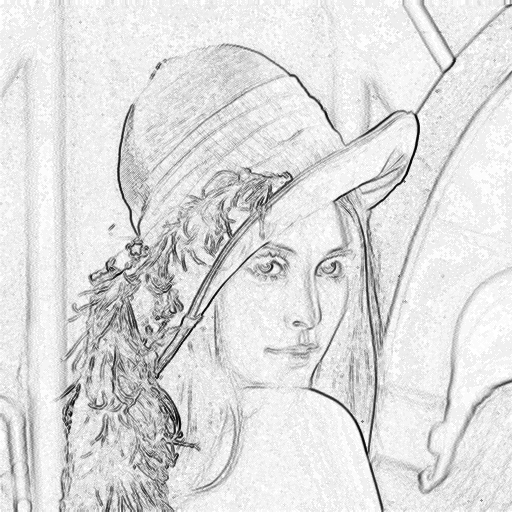
\includegraphics[width=.2\linewidth]{figs/geninput-000b}}  &
    \fbox{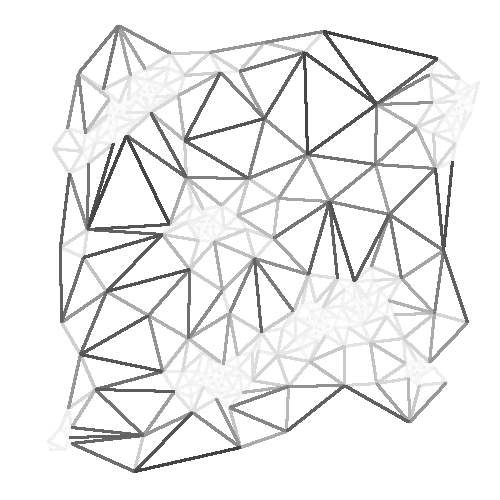
\includegraphics[width=.2\linewidth]{figs/geninput-001b}}  &
    \fbox{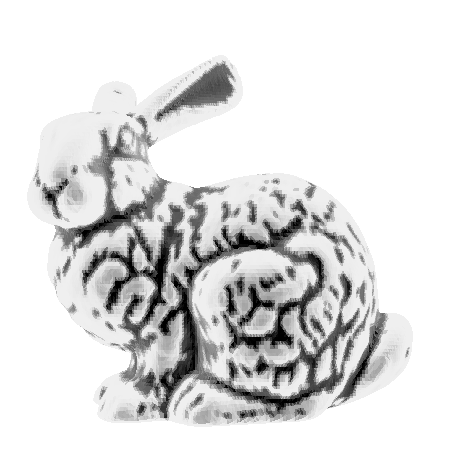
\includegraphics[width=.2\linewidth]{figs/geninput-002b}}
    \\[5pt]
    %
    output:                                                          &
    \fbox{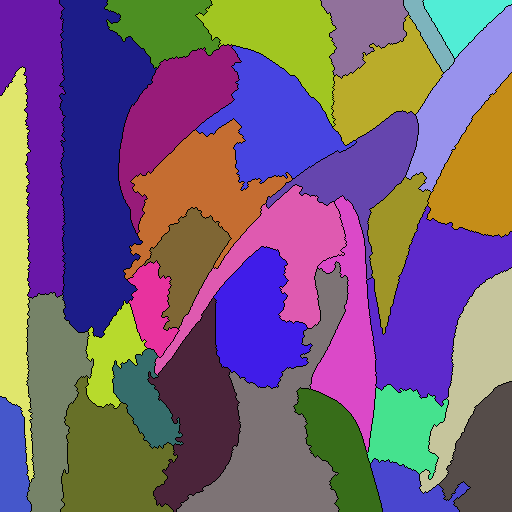
\includegraphics[width=.2\linewidth]{figs/genoutput-000}}  &
    \fbox{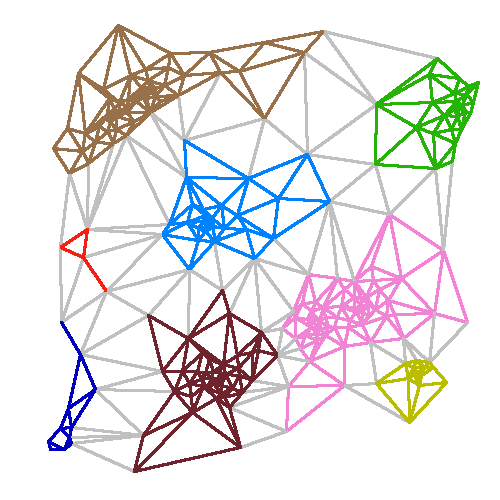
\includegraphics[width=.2\linewidth]{figs/genoutput-001b}} &
    \fbox{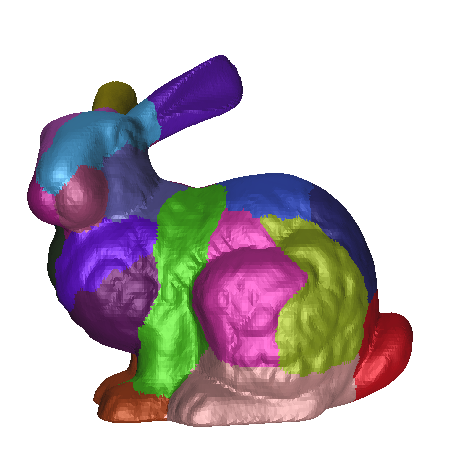
\includegraphics[width=.2\linewidth]{figs/genoutput-002b}}
    \\
  \end{tabular}
  \bigskip

  \text{The same code run on all these input.}

  \caption{Watershed algorithm applied to three different image types.}
  \label{fig:type.vs.algo}
\end{figure}

In image processing, there are three main axes around which genericity is applying. The first axis is about the data type:
grey level or RGB color (8-bits, 10-bits), decimal (double) and so on. The second axis, is about the structure of the
image: a contiguous buffer (2D or 3D), a graph, a look-up table and so on. Finally, the third axis is about additional
data that can be fed to image processing algorithms: structuring element (disc, ball, square, cube), labels
(classification), maps, border information and so on. In the end, an image is just a point within this space of
possibilities, illustrated in~\ref{fig:gen.espaceSAV}. Nowadays, it is not reasonable to have specific code for every
existing possibility within this space. It is all the more true when one wants efficiency.

\begin{figure}[tbh]
  \centering
  \subfloat[]{\includestandalone[width=1.7in]{figs/espaceSeI}}
  \hfil
  \subfloat[]{\includestandalone[width=1.7in]{figs/espaceSAV}}
  \caption{The space of possible implementation of the \emph{dilation(image, se)} routine. The image axis shown in (a)
    is in-fact multidimensional and should be considered 2D as in (b).}
  \label{fig:gen.espaceSAV}
\end{figure}

Genericity is not new and was first introduced in 1988 by Musser et al.~\cite{musser.1988.generic}. The main point is to
dissociate data structures and algorithms. The more your data structures and algorithms are tied together, the less you
will be generic and will fail to handle multiple data structures in the same algorithm. Further work has been made about
genericity in~\cite{musser.1994.algorithm, dehnert.1998.fundamentals}. Those works highlight the notion of abstraction
to be able to turn an algorithm tied to a data structure into a generic algorithm. Notably
in~\cite{stepanov.2009.elements}, Stepanov digs further and introduce the notion of \emph{Concepts}, which are static
requirements about the behavior of a type, by showing how to design a generic library and its algorithms. He highlights
the importance of having the algorithms driving the behavior requirements, and not the opposite. These works are very
suitable to be applied in the area of Image processing where we typically have a lot of algorithms (also called
operators) that are required to work on a lot of different data structures (also called image types).

The authors explain in~\cite{roynard.2019.rrpr} how to capitalize on those works to turn a data-structure-specific image
processing algorithm into a generic algorithm. We also explain how \emph{concepts} can ease the implementation of
generic algorithms. This approach is implemented in a library~\cite{carlinet.2018.pylena} which allows us to provide a
proof of concept over the feasibility of having generic image processing operators running on multiple image types with
near-native performances. Let us first explain briefly how we achieved this.

\subsection{Different approaches to get genericity}
\label{subsec:different.approaches}

First, let us consider the morphological \emph{dilation} that takes two inputs: an image and a flat structuring element
(SE). The set of some possible inputs is depicted in~\ref{fig:gen.espaceSAV}. Without genericity, with $s$ the
number of image type, $v$ the number of value type and $k$ the number of structuring elements, one would have to write
$s * v * k$ different \emph{dilation} routine.

There are several ways to reach a high level of genericity. First there are the \emph{code duplication} approach as well
as the \emph{generalization} approach. Finally, there is a way that consists in using expert, domain specific tools
specifically engineered for this purpose and build upon them: those tools usually make heavy usage of \emph{inclusion
  \& parametric polymorphism}, also known as template metaprogramming in C++, to provide the basic bricks the user needs
to build upon.

\paragraph{Code duplication approach} consists in writing and optimizing the algorithm for a particular type in mind.
Then, each time a new type is introduced, all the algorithm must be rewritten for this specific type. Additionally, each
time a new algorithm is introduced, it must support all the existing types and thus be written multiple times. This
approach does not scale well when the complexity of algorithms grows, and the number of data types increases. Neither it
does allow the implementer to easily make use of optimization opportunities that can be offered by different data types
having a common property. This translates into heavy switch/case statement in the code as show in~\ref{code:gen.exhau}
that illustrate how the \emph{fill} algorithm needs to dispatch according to the input data type.

\begin{figure}[tbh]
  \centering
  \begin{minted}[linenos,xleftmargin=17pt,gobble=2]{cpp}
  // image types parametrized by their
  // underlying value type
  template <ValueType V> struct image2d<V> { /* ... */ };
  template <ValueType V> struct image_lut<V> {/* ... */};
  // ...
  void fill(any_image img, any_value v)
  {
    switch((img.structure_kind, img.value_kind))
    {
    case (BUFFER2D, UINT8):
      fill_img2d_uint8( (image2d<uint8>) img,
                        (uint8) any_value );
    // ...
    case (LUT, RGB8):
      fill_lut_rgb8( (image_lut<rgb8>) img,
                     (rgb8) any_value );
    }
  }
  \end{minted}
  \caption{Fill algorithm skeleton with a switch/case dispatcher to ensure exhaustivity.}
  \label{code:gen.exhau}
\end{figure}

In addition, it is important to note that the exhaustivity aspect is only illustrated regarding the data structure types
here. Indeed, the data structures are all already generic for their underlying data type (named \emph{ValueType} in the
code). When one write \texttt{image2d<uint8>} (l.10), it means \emph{2D-image whose pixels' have a single channel 8-bits
  value}. This approach enables one to write an algorithm at maximum efficiency for a particular data type, however one
can easily miss optimization opportunities if not knowledgeable enough too. This approach is best for early prototypes
and trying to find common behaviors pattern among algorithms, or common properties across different data types. No IP
library has chosen this approach due to the obvious maintenance issue induced.

\paragraph{Generalization approach} consists in finding a common denominator to all the image types. Once designed, this
common denominator, also called supertype, can store informations about all the supported image types by the library.
This supertyp allows the library developer to write all the algorithms only once: for the supertype. The processing
pipeline will then consist in three steps. First convert the input image type into the supertype, second process the
supertype into the algorithm pipeline requested by the user, finally convert back the resulting image into the specific
image type the user is expecting. This approach offers the advantage of being maintainable. Adding a new image type is
just a matter of providing the two conversions facilities: to and from the supertype. Adding an algorithm is also just a
matter of writing it once for the supertype. This mechanism is shown in~\ref{code:gen.generalized}. However, one must
keep in mind that the conversion can be costly. Also, processing the supertype may induce a significant performance
trade-off while processing the original type would be much faster. Furthermore, it is not always possible to find this
common denominator when enumerating through some esoteric data types. Finally, the provided interface (from the
supertype) may allow the image to be used incorrectly, such as a $2D$ image being processed into video ($3D+t$)
algorithm. Widely use libraries such as OpenCV~\cite{bradski.2000.opencv}, scikit-image~\cite{vanderwalt.2014.skimage}
use this technique to handle as many image types as possible. Another library making use of this generalization
technique in its implementation is CImg~\cite{tschumperle.2012.cimg}. CImg generalize its data type to a 4D image type
templated by its underlying data type.

\begin{figure}[tbh]
  \centering
  \begin{minted}[gobble=2]{cpp}
  struct image4D { // generalized supertype
    // generalized underlying value-type
    // every value is converted to this one
    using value_type = std::array<double, 4>;
    /* ... */
   };
  // specific types w/ conversion routines
  struct image2D { image4D to(); void from(image4D); };
  struct image3D { image4D to(); void from(image4D); };
  // ...
  void fill(image4D img, const std::array<double, 4>& v) {
    for(auto p : img.pixels())
      p.val() = v;
  }
  \end{minted}
  \caption{Fill algorithm for a generalized supertype.}
  \label{code:gen.generalized}
\end{figure}

\paragraph{Inclusion \& Parametric polymorphism approach} consist in extracting behavior patterns from algorithms to
group them into logical brick called \emph{concepts} (for static parametric polymorphism), or \emph{interface} (for
dynamic inclusion polymorphism). Each algorithm will require a set of behavior pattern that the inputs need to satisfy.
In C++, it can be done either by using inclusion polymorphism, or by using parametric polymorphism, as shown
in~\ref{code:gen.inclupoly}. In~\cite{roynard.2019.rrpr}, we leverage a new C++20 feature (the concept) to show how it
is possible to turn an algorithm, specific to an image type, into a more abstract, generic one that does not induce any
performance loss. This approach, especially applied to image processing, will be seen more in-depth
in~\cref{chap:image.algorithms.taxonomy}.

\begin{figure}[htb]
  \centering
  \subfloat{
    \includegraphics[width=1.64in]{figs/inclupoly}
  }
  \hfil
  \subfloat{
    \includegraphics[width=1.64in]{figs/parapoly}
  }
  \vfil
  \subfloat[]{
    \includegraphics[width=1.64in]{figs/inclupoly_code}
  }
  \hfil
  \subfloat[]{
    \includegraphics[width=1.64in]{figs/parapoly_code}
  }
  \caption{Dynamic, object-oriented polymorphism (a) vs. static, parametric polymorphism (b).}
  \label{code:gen.inclupoly}
\end{figure}

Multiple libraries exist and leverage this approach to try to achieve a high genericity degree as well as high
performance by offering varied abstract facilities over image types and underlying data types. Those are
ITK~\cite{johnson.2013.ITKSoftwareGuideThirdEdition}, Boost.GIL~\cite{bourdev.2006.bgil},
Vigra~\cite{kothe.2011.generic}, GrAL~\cite{berti.2006.gral}, DGTal~\cite{coeurjolly.2016.dgtal},
Milena~\cite{levillain.2009.ismm,levillain.2010.icip},
Olena~\cite{olena.2000.www,levillain.2011.phd,geraud.2012.hdr,levillain.2014.ciarp} and
Pylena~\cite{carlinet.2018.pylena}. Most of them have been written in complex C++ whose details remain visible from the
user standpoint and thus are often difficult and complex to handle. It is also harder to debug because errors in highly
templated code shows up very deep in compiler error trace.

The table comparing all the pros. and cons. from the aforementioned approaches is presented
in~\cref{table:gen.approaches}.

\begin{table}[tbh]
  \centering
  \begin{threeparttable}
    \caption{Genericity approaches: pros. \& cons.}
    \begin{tabular}[width=0.8\linewidth]{l|ccccc}
      Paradigm             & TC      & CS      & E       & One IA & EA      \\
      \hline
      Code Duplication     & \cmark  & \xmark  & \cmark  & \xmark & \xmark  \\
      Code Generalization  & \xmark  & \eqmark & \eqmark & \cmark & \xmark  \\
      Object-Orientation   & \eqmark & \cmark  & \xmark  & \cmark & \cmark  \\
      Generic Programming: &         &         &         &        &         \\
      \quad with C++11     & \cmark  & \eqmark & \cmark  & \cmark & \eqmark \\
      \quad with C++17     & \cmark  & \cmark  & \cmark  & \cmark & \eqmark \\
      \quad with C++20     & \cmark  & \cmark  & \cmark  & \cmark & \cmark  \\
    \end{tabular}
    \begin{tablenotes}
      \item TC: type checking; CS: code simplicity; E: efficiency
      \item One IA: one implementation per algorithm; EA: explicit abstractions / constrained genericity
    \end{tablenotes}
    \label{table:gen.approaches}
  \end{threeparttable}
\end{table}

We can see in this table that Generic Programming in C++20 check all the boxes that we are interested in.

\FIXME{Discussion à propos du tableaux : motivé avec des exemples les principaux points}

\subsection{Unjustified limitations}
\label{subsec:limitations}

Image processing community operates mostly with either Python or Matlab~\cite{etter.2002.introduction}. As such this
subsection will focus on those two technologies. Python offers access to two major libraries for image processing:
OpenCV and scikit-image. Matlab has built-in support as well as toolboxes for more advanced features. When we intersect
scikit-image and Matlab, we can notice that both are very similar both in feature and interface. As such, it is possible
to regroup them both here for the sake of comprehension. As stated above, when considering a generic library, one must
consider the three axes: underlying data type, domain structure and additional data. Let us compare how the mentioned
library behave along those axes with a simple algorithm such as the morphological dilation.

\subsubsection{Limitations regarding feasibility}

\paragraph{Data type} Dilating a grayscale or a binary image works fine as intended with all the libraries. However,
there is no trivial way of dilating a RGB colored image~\parencite{angulo.2007.morpho_color,dewitte.2005.morpho_color}
as this operation is not defined for colored images. Indeed, the algorithm is able to work if a supremum function is
provided. Such functions have multiple possible implementation and selecting the correct one is not trivial. However,
provided a supremum function, the dilation algorithm should normally be performed. Despite that fact, scikit-image does
not allow one to dilate a colored RGB image and raises an error: it is required to convert into a grayscale the image
beforehand.

OpenCV arbitrarily decides that the colored dilation consists in dilating each channel of the colored image separately
from one another. It is effectively selecting a partial marginal order relation under the hood. This arbitrary choice
may cause false colors to appear in the resulting image (which most of the time is not what the user wants).
Furthermore, it is not possible to provide a supremum function to the dilation algorithm to customize the behavior which
is a server drawback.

\paragraph{Domain structure} To perform a dilation, it is required to have a structuring element whose shape matches the
structure of the domain of the image. For instance, dilating a 2D-image requires the use of a structuring element whose
shape may be a disc or a rectangle. To dilate a 3D-image, one would need to use a structuring element whose shape is of
a ball or a cube. Scikit-image supports 3D-images as well as structuring element whose shape are compatible (ball,
rectangle and octahedron). This naturally leads to having a support for the dilation of 3D-images. On the other hand,
OpenCV does support 3D-images whereas its dilation algorithm cannot handle them. The algorithm exits with an error.
Worse, when passing a wrong structuring element (a rectangle) to the dilation algorithm alongside the 3D-image, the
algorithm works and produce a result which is false: it is similar to the application of the 2D-structuring element on
each 2D-slice of the 3D-image.


\subsubsection{Limitations regarding optimizations}

Each library has its own strategies to optimize its routines when implementing them.

\paragraph{Scikit-image} for instance, will check whether the structuring element is separable (only for
rectangle shapes) so that it can dispatch on an optimized multi-pass 1D routine for each part separated which linearize
the execution time and greatly improve performances for large structuring element.

Also, Scikit-image relies on SciPy internals which does not abstract the underlying data type for the algorithm
implementer. As such, each algorithm must provide a switch/case dispatch for every supported type (floating points,
8-bit channel, 16-bit channel, RGB, etc.), and it must provide it in the middle of the algorithm implementation. If one
type is not natively supported; an error occurs and the program halts. Henceforth, handling a new supported data type
will requires to review every single written algorithm.

On the other hand, SciPy provides an abstraction layer over the dimensional aspect of the image by providing a tool
named point iterator. This tool allows one to iterate over every point of the image, without being aware of the number
of its dimension, and make the translation from the abstract iterator to the actual offset in the data buffer of the
image. The implementer can then only worry about handling the underlying data type to provide a generic algorithm. This
approach, sadly, is fully dynamic (that is, runtime) and does not allow the compiler to provide native optimization such
as vectorization out of the box.

\paragraph{OpenCV \& Matlab} In OpenCV as well as in Matlab, the choice was made to systematically attempt to decompose
big rectangular structuring elements into smaller $3*3$ structuring elements. This is not as effective as using
multi-pass 1D algorithm but still allows for relatively stable performances.

Also, OpenCV let the implementer handle the cases he wants to support by himself. For instance, the dilation algorithm
is written with a dispatch on the data type before the actual call to the algorithm. This enables compiler optimizations
such as vectorization because all the required information is known at the right time. It also enables offloading the
computation into GPU kernels when feasible. However, the downside is that few algorithms are written in a way to handle
multidimensional images. Most are written to only handle specific subsets. As such, conversion from one subset to
another may be unavoidable when writing an algorithm pipeline for a more complex application. For instance, it is
currently not possible to dilate a 3D image with a 3D ball (as stated above).

Another point to note with OpenCV is the requirement to do temporary copies (to extract data or to have working copy)
when writing an algorithm. For instance, it is currently not possible to write a dilation algorithm operating only on
the green channel of an RGB image. One must first extract the green channel into a single channel temporary image, blur
that image, to finally put the result back into the original image. Generally, \FIXME{in-place?} computation is poorly
handled in OpenCV.

\paragraph{Performance discussion} When comparing performances of the simple dilation between Matlab and OpenCV, which
is done in~\cite{matuska.2012.bench}, shows that Matlab is very oriented toward prototyping and not toward production.
The performance gap between the two libraries shows that performances may not a major concern for MatLab in this case.
Opposite to this, OpenCV and scikit-image both have a C/C++ core to provide fast basic algorithms such as the dilation
and erosion mathematical morphology.

As such, when comparing the performances of OpenCV, Scikit-image and Pylene in~\cref{fig:gen.bench.square.disc}, we can
notice some interesting facts. Both scikit-image and Pylene have a very stable execution time even though the size of
the structuring element grows by power of two. This corroborates the fact that the author did see code taking advantage
of the structuring element's properties, such as the decomposability/separability. OpenCV has very good performances for
a square because it has specific handwritten code for both vectorization and GPU offloading when possible: even if
OpenCV decomposed its square into smaller sub square (and not periodic lines), it remains steady fast.

\begin{figure}[htb]
  \centering
  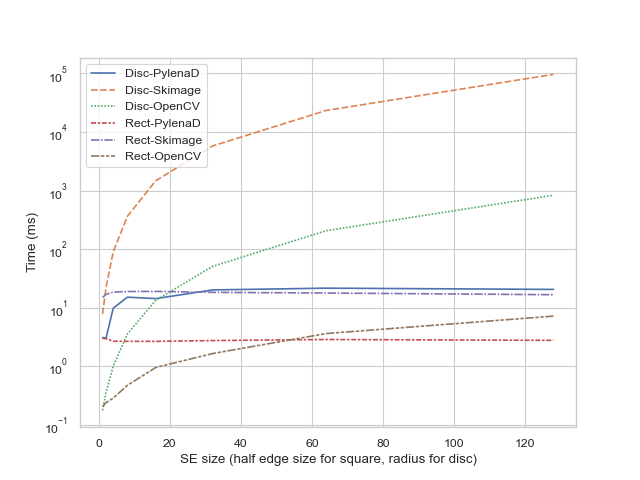
\includegraphics[width=3.8in]{figs/bench_disc_rect_by_SE}
  \caption{Benchmark: dilation of a 2D image (3128x3128 \eqmark 10Mpix) with a 2D square and a 2D disc. \FIXME{Légende image (noms, espace)}}
  \label{fig:gen.bench.square.disc}
\end{figure}



In the case of a structuring element shaped as a disc (also in~\cref{fig:gen.bench.square.disc}), we can observe that
the execution time raises exponentially for both Scikit-image and OpenCV whereas Pylene remains regular and steady fast.
These results show that Pylene's attempt to decompose each structuring element into periodic lines when possible may be
slightly slower for smaller structuring elements whereas it is much more regular and faster when the structuring element
start to be of a certain size.

\FIXME{Rajouter arbre de décision de l'algorithme final qui tourne sur chaque bibliothèque ave cnote sur les méthodes de décisions (statiques ou dynamique)}

\subsubsection{Limitations regarding static types in a dynamic world}

Being statically typed (at language level) has its advantages (performance, optimization) but also has sever drawbacks,
especially when interfacing with dynamic languages such as Python. Indeed, being statically typed in a dynamic world
disqualify the library from being able to select, for instance, a new, custom structuring element, when performing a
dilation. Indeed, all the supported structuring elements must be listed in advance and code must be compiled for each
supported type. This induce a strong inertia when the practitioner wants to try out new things not yet supported by the
library. This also defeats the initial purpose of being generic. Indeed, one would expect a generic library to work with
any type and not jst a specified set of pre-compiled types. Being able to break through this limit is addressed more
in-depth in~\cref{chap:static_dynamic_bridge}.


\FIXME{Conclusion vis-à-vis de la généricité: un algo générique est plus rapide ? La généricité ne nuit pas aux
  performances ? La généricité permet de dispatcher plus facilement ?}


\section{Genericity within programming language}
\label{sec:gen.genericity.within.programming.languages}

Genericity is a more than 45 years old notion. It was first introduced alongside the CLU language in 1974 by Barbara
Liskov and her students~\parencite{liskov.1993.cluart}. The language offered many features such as data encapsulation,
iterators and especially \emph{parametrized modules}. A module in CLU is represented by a \emph{cluster}. A
\emph{cluster} is a programming unit grouping a data structure and its related operations. In modern programming, we
would call it a class where the data structure correspond to the member variables and the operations correspond to the
member functions (or methods). In CLU, the clusters can be parametrized which is a way to introduce the notion of
parametric polymorphism. Indeed, clusters offered the ability to define a generic data structure and its functions whose
behavior will not change whatever type the cluster is parametrized with. At first, type-safety was enforced at run-time
in CLU. Later, \emph{where clauses} were introduced to specify specific requirements over cluster type parameters. This
had the consequence of allowing only the operations required in the where clause to be used in the cluster
implementation code. This enables proper compile-type checks, type-safety and the compilation into a simple native and
optimized code by the compiler. The following code illustrate how to create a cluster (or class) named \emph{vector},
declaring a set of member functions and requiring a specific behavior (operator $=$ and $<$) from its underlying stored
elements:

\begin{minted}{cobol}
  vector = cluster [T: type] is
    create, size, contains, sort, remove, push_back
  where
    T has equal: prototype(T, T) return (bool)
    T has less: prototype(T, T) return (bool)
\end{minted}

When implementing the member functions declared for \texttt{vector}, the only valid operations that can be performed on
a value of type \texttt{T} are \texttt{equal} ($=$ for comparison) and \texttt{less} ($<$ for ordering). In CLU the
actual instantiation of the parameter (here \texttt{T}) is done at run-time. Indeed, each type is represented by a
descriptor, even a parametrized type parameter. At run-time, a concrete type is used to instantiate the cluster. To
achieve this, the placeholder type descriptor is replaced by the one of the actual concrete type at this moment. The
instantiation can then be considered dynamic which differs from the C++ compilation model where the template
instantiation is considered static (i.e. done at compile-time). The pros and cons of this approach are discussed
in~\parencite{atkinson.1978.cluimpl} which essentially are the resulting binary code size due to combinatorial explosion
combined with optimized code generation versus small, flexible and slower binary.

Later on came the Ada programming language whose conception work started in 1977 and first version was released in 1980.
It was first standardized in 1983~\parencite{ansi.1983.ada} in the United States by the American National Standards
Institute (ANSI) before being Internationally standardized by the International Organization for Standardization (ISO)
in 1987~\parencite{iso.1987.ada}. From this point on, the Ada language released a new version in
1995~\parencite{iso.1995.ada, iso.1995.ada.corr}, then the standard committee published an Amendment in
2007~\parencite{iso.1995.ada.amend} which is often referred as Ada 2005. Finally, a new version of the language was
published in 2012~\parencite{iso.2012.ada,iso.2012.ada.corr}. What interest us in the Ada language is the fact that the
language features \emph{generics} since it was first designed in 1977-1980 which \emph{ten years} before Musser and
Stepanov published their first work about genericity in 1988~\parencite{musser.1988.generic}. Indeed, it took around 20
years for the fist Standard Template Library (STL) will then be standardized in the C++ programming language in
C++98~\parencite{iso.1998.cpp}. It then took almost 10 more years for an STL to land into the Ada programming language in
the 2007 Amendment for Ada 2005.

In the Ada programming language, it is possible to mark a package or a procedure as generic with the \texttt{generic}
keyword. The developer then lists the parametrized parameter the package and/or the function requires to be implemented.
The following code demonstrates how this feature work by implementing a function replacing the first argument by a new
value and returning its previous value (also known as exchange).

\begin{minted}{Ada}
generic
  type T is private;
function exchange (x : in out T; v : in T) return T is
  tmp : T;
begin
  tmp := x;
  x   := v;
  return tmp;
end exchange;
\end{minted}

In Ada, generic packages and routines (procedures, functions) must be instantiated explicitly: the compiler cannot infer
the parametrized type at compile time from the context of use (whereas a C++ compiler can). Thus, the following three
lines must be written explicitly for the compiler to generate the binary code of the above function:
\begin{minted}{ada}
  function int_exchange is new exchange (Integer);
  function float_exchange is new exchange (Float);
  function str_exchange is new exchange (String);
\end{minted}

In Ada, this model enables the possibility of sharing a generic across several compilation units since its compilation is
independent of its use whereas in C++, until C++20 the sharing model consists in copy-pasting the whole source code
(and transitive recursive dependencies) each time a generic (a template) code is compiled. C++20 (standardized in 2020,
42 years after C++98) bring a solution to this issue by standardizing C++ modules. However, this feature is out of scope
of this study and will not be discussed in this thesis.

Also, Ada support syntactic constraints on parameters similar to the CLU language. It is translated into a \texttt{with}
clause listing the constraints on the parameter(s). The following code shows how to implement such a constrained generic
function by using the mathematical maximum operator as an example:

\begin{minted}{ada}
generic
  type T is private;
  with function "<" (x, y: T) return Boolean is <>;
function maximum (x, y : in T) return T is
  tmp : T;
begin
  if x < y then
    return x;
  else
    return y;
  end if;
end maximum;
\end{minted}

Let us not forget to instantiate the constrained generic function for integers:

\begin{minted}{ada}
  function int_maximum is new maximum (Integer);
\end{minted}

This idea of constrained generic is 30 years old and has only made his way very recently (2020) in the C++ programming
language under the feature name of \emph{concepts}.

Now that we have introduced where generic programming is coming from, let us focus on the C++ programming language and
how it has made his way into the language along the last 30 years, as well as along the years to come.

\subsection{Genericity in pre C++11}
\label{sec:precpp11}

Before C++11~\parencite{iso.2011.cpp} came out the genericity facilities offered by the C++ programming language were
already Turing-complete~\parencite{veldhuizen.2003.c++templates}. However, it was lacking a certain amount of features
the language now have that made writing generic code a real challenge at that time. For instance, when writing code with
a variable number of types (nowadays designated as variadic templates) one had to write the generic code for each and
every number of type supported. This meant that to implement \texttt{std::tuple}, one had to copy the implementation for
every number of type supported by \texttt{std::tuple}. This limitation defeated the very first principle and motivation
of generic programming which is to write \emph{less} Code. To compensate, library implementers used tricks with macro
not to have to rewrite code which made the initial code even harder to understand for outsiders.


\subsubsection{Functions on types (or traits)}

The very first feature every developer writing metaprogramming C++ code has used is called \emph{type-traits}. Those
\emph{traits} are a way to mutate a type depending on the way a template declared on a data structure is resolved.
Indeed, in C++ the instantiation of a template depends on the context, which means the compiler is required to build a
set of possible way to resolve a template instantiation and in order to determine the best match to resolve the
instantiation. This mechanism is well known and documented in the C++ standard, it can then be used (and abused) to do a
great number of things. Among all the traits that exist (a lot of them have been standardized in C++11, 2011, in the
header \texttt{<type\_traits>}), some in particular are used in every codebase: \texttt{remove\_const},
\texttt{remove\_volatile} and \texttt{remove\_reference}. Let us see how they are implemented:

\begin{minted}{C++}
  template<class T> struct remove_const                { using type = T; };
  template<class T> struct remove_const<const T>       { using type = T; };
  
  template<class T> struct remove_volatile             { using type = T; };
  template<class T> struct remove_volatile<volatile T> { using type = T; };

  template<class T> struct remove_reference            { using type = T; };
  template<class T> struct remove_reference<T &>       { using type = T; };
  template<class T> struct remove_reference<T &&>      { using type = T; };
\end{minted}

For \texttt{remove\_const}, first is defined the structure whose underlying alias \texttt{type} points to the passed
template parameter \texttt{T}. Then we define a template specialization whose matching parameters are all \texttt{T}
parameters that are \texttt{const}. The defined underlying alias \texttt{type} for this specialization then is
\texttt{T} without the qualifying \texttt{const}. This way, there are two possibilities when calling this \texttt{trait}
(or metafunction): either the passed parameter is not \texttt{const} which means it will be forwarded as-is to the
underlying alias \texttt{type} or the passed parameter is \texttt{const} which means the underlying alias \texttt{type}
will be defined by dropping the \texttt{const-qualifier} off of the passed parameter type. For instance:

\begin{minted}{C++}
  using T1 = remove_const<double>::type // T1 is double
  using T2 = remove_const<const double>::type // T2 is double too, const-qualifier is dropped
\end{minted}

This language construct is very useful when developing generic libraries because it enables performing "functions" on
types, and even chain them. It is also possible to perform checks to extract information about those types. We can
easily write a \texttt{is\_const} metafunction if we need it.

In image processing in particular, the usage of traits in the generic library
Milena~\parencite{levillain.2009.ismm,levillain.2010.icip} was very useful to achieve standard ways to compute very
useful types from other complex type. From the image processing definition of an image type, we can already see a number
of traits that a generic library would want to provide. Indeed, it would be useful to be able to extract the type of the
domain (box2d, box3d, etc.), the type of the point (point2d, point3d, ...), the underlying value type (uint8, rgb8,
etc.) and so on. We can also already see emerging consistency issues between those types. Indeed, a box3d domain would
not accept access via a point2D. It would instead require a point3d. All those issues will be addressed later in
the~\cref{chap:image.algorithms.taxonomy}. However, we can already give here minimal working example as to how type
traits are especially useful in a generic image processing library. First let us define some minimal data structures:

\begin{minted}{C++}
  struct point2d {int x, y; };
  string rgb8 { uint8_t r, g, b; };
  struct box2d {
    using value_type = point2D;
    // ...
  };
  struct image2d {
    using domain_type = box2d;
    using point_type  = point2d;
    using value_type  = rgb8;
    // ...
  };
\end{minted}

Now we would want to implement \texttt{traits} to extract type information from those structures. Here is how we do it
in a generic library:

\begin{minted}{C++}
  template <class T> struct domain_value_type { using type = typename T::value_type;  };
  template <class T> struct image_point_type  { using type = typename T::point_type;  };
  template <class T> struct image_value_type  { using type = typename T::value_type;  };
  template <class T> struct image_domain_type { using type = typename T::domain_type; };
\end{minted}

These traits extract information about types in a generic way and can be used in any algorithm taking an image as a
template parameter. For instance, here is how an image processing algorithm (trivially extracting the max value) would b
e written:

\begin{minted}{C++}
template <class Ima>
typename image_value_type<Ima>::type // usage of trait
min_value(const Ima& ima) {
  using value_t = typename image_value_type<Ima>::type; // usage of trait
  auto min = std::numeric_limits<value_t>::max();
  for(auto v : ima.values()) {
    auto min = std::min(min, v);
  }
  return min;
}
\end{minted}

\subsubsection{SFINAE: Substitution-Failure-Is-Not-An-Error}
\label{subsec:sfinae}

Additionnaly, another feature related to metaprogramming  allowed the developer to design generic libraries: the
SFINAE~\parencite{vandevoorde.2002.c++} (substitution-failure-is-not-an-error) technique that leads to the
popularization of the usage of the \texttt{std::enable\_if} metaprogramming construct. The SFINAE technique relies on a
feature of the C++ programming language. Indeed, when standardizing how the compiler should resolve and select function
overloads, in a templated context, the standard committee chose to have the following behavior: "when substituting the
explicitly specified or deduced type for the template parameter fails, the specialization (function overload candidate)
is discarded from the overload set (of matching functions) instead of causing an error".

This feature allows writing code that seem to be ill-formed, for instance in a function, trying to access a class member
type, variable or function that does not exist should be ill-formed. However, because it happens in a templated context
during the instantiation resolution, when the compiler tries to instantiate a function template with a parametrized
type, the compiler will just discard the function from the overload resolution set at call-site instead of throwing a
hard error. An error can occur only when the compiler tried all the overload it knows in the overload set and still
could not find an overload that was not ill-formed. If this happens, the compiler will then proceed to list all the
overloads it tried, to list all the template substitution it tried and finally to list why it failed. This mechanism is
the very reason of the unpopularity of this technique because it leads to situation where the compiler can output
\emph{several Mos} of error message for one single file. Error messages become incomprehensible very fast and programs
are hard to debug because everythFor instance, here is some real-world example extracted from generic image prcessing
code that allows implementing the \emph{fill} algorithm in two very different ways depending on how behaves the input
image type:ing happens at compile-time. But still, it was the only technique we had to perform any kind of detections on
types at compile time to require some any given constraints on them.

For instance, here is some real-world example extracted from generic image processing code that allows implementing the
\emph{fill} algorithm in two very different ways depending on how behaves the input image type. First we need to write
the detector which is a structure whose templated context will be ill-formed during template instantiation. This
detector will inherit either \texttt{std::true\_type} or \texttt{false\_type} depending on whether the detection is
successful or not:

\begin{minted}{C++}
  // Step 1 write detector
  template <class Ima, class = void>
  struct is_image_with_lut : std::false_type {};

  template <class Ima>
  struct is_image_with_lut<Ima,
     typename Ima::lut_type // constraint over the existence of the lut_type field
  > : std::true_type {};
\end{minted}

Now let us introduce a new image type for the sake of this example:

\begin{minted}{C++}
  struct image2d_lut : image2d {
    using lut_type = std::array<uint8_t, 256>;
    using value_type = uint8_t:
    lut_type& get_lut();
  };
  template <class Ima>
  struct image_lut_type {
    using type = typename Ima::lut_type;
  }
\end{minted}

The next step is to implement the \texttt{enable\_if} facility. This is included in the C++ STL starting from C++11 and
onward:

\begin{minted}{C++}
  template<bool B, class = void>
  struct enable_if {};

  template<class T>
  struct enable_if<true, T> {
    using type = T;
  };
\end{minted}

Now we are all set to use all those construct to dispatch our algorithms from call-site depending on our input image
type:

\begin{minted}{C++}
  // Overload #1 : with lut
  template <class Ima, 
  void fill(Ima& ima, typename image_value_type<Ima>::type val,
            typename enable_if<is_image_with_lut<Ima>::type::value, void*>::type = 0)
  { // Image with lut
    using lut_t = typename image_lut_type<Ima>::type;
    using value_t = typename image_value_type<Ima>::type;
    lut_t& lut = ima.get_lut();
    for(value_t& v : lut)
      v = val;
  }

  // Overload #2 : without lut
  template <class Ima, 
  void fill(Ima& ima, typename image_value_type<Ima>::type val,
            typename enable_if<not is_image_with_lut<Ima>::type::value, void*>::type = 0)
  { // Image without lut
    using value_t = typename image_value_type<Ima>::type;
    for(value_t& v : ima.values())
      v = val;
  }
\end{minted}

Finally, let us give some call-site example to finish illustrating our point:

\begin{minted}{C++}
  image2d_lut ima1;
  image2d ima2;

  fill(ima1, 0);   // will dispatch over overload #1
  fill(ima2, 255); // will dispatch over overload #2
\end{minted}
Here, no hard error occur. Both overload are dispatched according to the constraint built with the SFINAE construct. Now
we can talk about \emph{constrained genericity} in C++.


\subsection{CRTP: Curiously Recurring Template Pattern}
\label{subsec:crtp}

Another features that precede C++11 and was available in C++98~\parencite{iso.1998.cpp} and
C++03~\parencite{iso.2003.cpp} is the curiously recurring template pattern (CRTP) introduced in 1996 by
Coplien~\parencite{coplien.1996.crtp}. This programming technique allows a base class (in its specific code) to be aware
of its derived class at compile type. We made extensive use of this pattern in the past to design a new paradigm,
SCOOP~\parencite{burrus.2003.mpool, geraud.2006.scoop-pres, geraud.2008.mpool, levillain.2011.phd} which combined
multiple inheritance (via CRTP) and concept checking (via SFINAE) to implement a solution to provide a library with
constrained genericity in C++ for the image processing area. The Scoop paradigm relied on the fact that multiple
(especially diamond) inheritance did not pose much of an issue as long as there was no member variable involved. This
way, one could consider a class hierarchy as a hierarchy of constraint indeed. Using CRTP, it was possible to find back,
inside constraining classes, what was the concrete leaf class of the hierarchy in order to check whether its
implementation satisfied the constraints or not. For instance, let us assume that we have a concrete class
\texttt{image2d} inheriting from a constraining class \texttt{Image}. Let us now see how one would use the SCOOP
paradigm to implement it. First we need to implement the satellite constraints around the image type which are related
to the underlying point and domain of the image.

\begin{minted}{C++}
  template <class P>
  struct Point { // concept checking class
    int (P::*m_ptr1) const = & P::dim;
  };

  struct point2d : Point<point2d> { // CRTP
    int x, y;
    int dim() const { return 2; }
  };

  template <class D>
  struct Domain { // concept checking class
    using value_type = typename D::value_type;
    // ...
  };

  struct box2d : Domain<box2d> { // CRTP
    using value_type = point2d;
    // ...
  };
\end{minted}

For the sake of brevity, we are omitting the implementation of domain functions related to iterating over all the points
of the domain. With those concept defined, we can now dig into how we would implement an image class with the SCOOP
paradigm.

\begin{minted}{C++}

  template <class I>
  struct Image { // concept checking class
    using value_type = typename I::value_type;
    using point_type = Point<typename I::point_type>;
    using domain_type = Domain<typename I::domain_type>;

    const domain_type& (I::*m_ptr1)() const = & I::domain;
    // ...
  };

  struct image2d : Image<image2d> { // CRTP
    using value_type = uint8_t;
    using point_type = point2d;
    using domain_type = box2d;

    // ... ctors ...

    const domain_type& domain() const {
      return m_dom;
    }
  private:
    domain_type m_dom;
  };
\end{minted}

Each time a leaf class in the hierarchy inherit from a base class, the concepts are checked. The syntax is not really
intuitive, especially writing the function pointers to check that their prototype is confirming a certain behavior, but
it was all what was available at that time. To be completely exhaustive, the library implementing this paradigm,
Milena~\parencite{levillain.2010.icip, levillain.2009.ismm} featured another powerful tool which allows one to require
only concept class into input data for algorithms. Inside the algorithm it was then possible to get back the concrete
class and use it as if it was originally passed as an argument. To do so, it was needed to add a member field to the
concept class named \texttt{exact\_t} that kept track of the leaf class into the concept checking class.

\begin{minted}{C++}
  template <class I>
  class Image {
    // ...
    using exact_t = I;
  };
\end{minted}

Then a simple cast routine would do the trick inside the algorithm:

\begin{minted}{C++}
  #define EXACT(Ima) \
    typename Ima::exact_t
    
  template <class Ima> // mutable routine
  EXACT(Ima)& exact(Ima& ima) { return static_cast<EXACT(Ima)&>(ima); }

  template <class Ima> // const routine
  const EXACT(Ima)& exact(const Ima& ima) { return static_cast<const EXACT(Ima)&>(ima); }
\end{minted}

This way, in image processing algorithms, the implementer would only need to write minimal code for it to work out of
the box:

\begin{minted}{C++}
  template <class I>
  void fill(Image<I>& ima, typename image_value_type<Ima>::type val) {
    EXACT(Ima)& ima_ = exact(ima);

    // use the concrete underlying image ima_ and val
  }
\end{minted}

This constrained genericity would be totally transparent as shown with the following code that just works out of the
box, thanks to the SCOOP paradigm and its inheritance strategy to constrain classes.
\begin{minted}{C++}
  image2d ima = /* ... */;
  uint8_t val = 0;
  fill(ima, val);
\end{minted}

By extension, this work on Milena was integrated in the image processing platform
Olena~\parencite{olena.2000.www,geraud.2012.hdr}. This platform centralizes the work that was done around this field of
research for a long time~\parencite{geraud.2000.icpr,duretlutz.2000.olena,darbon.2002.ismm,darbon.2004.ecoopphd}. More
details can be found about SCOOP, and notably how it enables property based programming (augmentation of types via
properties) in the work of
\citeauthor{levillain.2011.phd}~\parencite{levillain.2011.phd,levillain.2009.ismm,levillain.2010.icip,levillain.2010.wadgmm,levillain.2011.gretsi,levillain.2011.phd,levillain.2012.wadgmm-lncs,levillain.2014.ciarp}.

Those approaches have the advantage of being really flexible and to be able to perform the concept checking work that we
wanted to have, be it to constrain implementation or to dispatch to the correct overloaded algorithms depending on
specific properties. The disadvantages come in the form of an increased complexity of the design hierarchy of
implemented types as they must inherit concepts via CRTP and conform to specific constrains. Also, all the
implementation is visible as all the code is generic (template) and all the implementation details are leaked to the
user code. For an image processing library which can use several dependencies (for instance, a library that read images
from disc from multiple image formats), this is a huge drawback.

With the release of new C++ standards in 2011~\parencite{iso.2011.cpp}, then 2014~\parencite{iso.2014.cpp},
2017~\parencite{iso.2017.cpp} where template metaprogramming facilities were greatly improved, it was necessary to
review once more this design to improve the design in order to achieve genericity, performance and ease of use. This is
the birth of a new library, Pylene~\parencite{carlinet.2018.pylena}. In the end, it was C++20~\parencite{iso.2011.cpp}
that marked the shift wanted by
Stepanov~\parencite{musser.1988.generic,musser.1994.algorithm,dehnert.1998.fundamentals,stepanov.2009.elements} and
Stroustrup~\parencite{stroustrup.1995.design,stroustrup.1999.hot,stroustrup.2003.concepts,stroustrup.2007.hopl} for
years with the coming of Concepts, and all the new possibilities it brings to the programmer.

\section{Genericity in post C++11 (C++20 and Concepts)}
\label{sec:postcpp11}

\begin{figure}[tbh]
  \centering
  \begin{minted}[linenos,xleftmargin=17pt,gobble=2,highlightlines={2,4,5}]{c++}
  template <Image Ima, ValueType Val>
    requires same<Ima::value_type, V>
  void fill(Ima ima, Val val) {
    for(Val v : ima)
      v = val;
  }
  \end{minted}

  \caption{Fill algorithm, generic implementation.}
  \label{code:gen.fill}
\end{figure}

Most of the algorithms are \emph{generic} by nature. What limits their genericity is the way they are implemented. This
statement is justified by the work achieved in the Standard Template Library (STL)~\parencite{dehnert.1998.fundamentals}
in C++ whose algorithms are implemented and designed in a way where they work with all the built-in collections (linked
list, vector, etc.). Let us take the example of the algorithm \texttt{fill(Collection c, Value v)} which set the same
value for all the element of a collection (see~\cref{code:gen.fill}). There are three main requirements here that are not
related to the underlying type of \emph{Collection}. First, we check (l.2~\ref{code:gen.fill}) that we are actually
filling the collection with the correct type of value. Indeed, it would not make sense, for instance, to assign an RGB
triplet color into a pixel from a grayscale image. Secondly, we need to be able to iterate over all the element of the
collection (l.4~\ref{code:gen.fill}). Finally, we need to be able to write a value into the collection
(l.5~\ref{code:gen.fill}). This requires the collection not to be read-only, or the collection's values not to be yielded
on-the-fly. This allows us to deduce what is called a \emph{concept}: a breakdown of all the requirement about the
behavior of our collection. When writing down what a \emph{concept} should require, one should always respect this rule:
\blockquote{\emph{It is not the types that define the concepts: it is the algorithms}}. Concepts in C++ are not new and
there have been a long work to introduce them that goes back from
2003~\parencite{seymour.2009.concepts,stroustrup.2003.concepts,sutton.2017.concepts} to finally appear in the 2020
standard~\cite{voutilainen.2017.concepts} (referred as C++20~\parencite{iso.2011.cpp}). This allows us, as of today, to
write code leveraging this facility.

\subsection{Conceptification}
\label{subsec:conceptification}

C++ is a multi-paradigm language that enables the developer to write code that can be \emph{object oriented},
\emph{procedural}, \emph{functional} and \emph{generic}. However, there were limitations that were mostly due to the
backward compatibility constraint as well as the zero-cost abstraction principle. In particular the \emph{generic
  programming} paradigm is provided by the \emph{template metaprogramming} machinery which can be rather obscure and
error-prone. Furthermore, when the code is incorrect, due to the nature of templates (and the way they are specified) it
is extremely difficult for a compiler to provide a clear and useful error message. To solve this issue, a new facility
named \emph{concepts} was brought to the language. It enables the developer to constraint types: we say that the type
\emph{models} the \emph{concept(s)}. For instance, to compare two images, a function \emph{compare} would restrict its
input image types to the ones whose value type provides the \emph{comparison operator ==}. In spite of the history
behind the \emph{concept checking} facilities being very
turbulent~\parencite{seymour.2009.concepts,stroustrup.2003.concepts,sutton.2017.concepts}, it will finally appear in the
next standard~\cite{voutilainen.2017.concepts} (C++20).

The C++ \emph{Standard Template Library} (STL) is a collection of algorithms and data structures that allow the
developer to code with generic facilities. For instance, there is a standard way to \emph{reduce} a collection of
elements: \texttt{std::accumulate} that is agnostic to the underlying collection type. The collection just needs to
provide a facility so that it can work. This facility is called \emph{iterator}. All STL algorithms behave this way: the
type is a template parameter so it can be anything. What is important is how this type behaves. Some collection requires
you to define a \texttt{hash} functions (\texttt{std::map}), some requires you to set an \emph{order} on your elements
(\texttt{std::set}) etc. This emphasis the power of genericity. The most important point to remember here (and explained
very early in 1988~\cite{musser.1988.generic}) is the answer to: \blockquote{\emph{What is a generic algorithm?}}. The
answer is: \blockquote{\emph{An algorithm is generic when it is expressed in the most abstract way possible}}. Later, in
his book~\cite{stepanov.2009.elements}, Stepanov explained the design decision behind those algorithms as well as an
important notion born in the early 2000s: the concepts. The most important point about concepts is that it constrains
the behavior. Henceforth: \blockquote{\emph{It is not the types that define the concepts: it is the algorithms}}. The
\emph{Image Processing} and \emph{Computer Vision} fields are facing this issue because there are a lot of algorithms, a
lot of different kinds of images and a lot of different kinds of requirements/properties for those algorithms to work.
In fact, when analyzing the algorithms, you can always extract those requirements in the form of one or several
\emph{concepts}. This section is a preface to the image taxonomy which will be seen more in-depth
in~\cref{chap:image.algorithms.taxonomy}.

Image processing algorithms, similarly, are \emph{generic} by
nature~\cite{ritter.1990.cvgi,geraud.2000.icpr,darbon.2002.ismm,levillain.2010.icip,levillain.2014.ciarp}. When writing
an image processing algorithm, there is always a way to express it with a high level of genericity. For instance, if is
possible to write a morphological dilation in a way that does not care about the underlying value type, the domain nor
the structuring element specificities. The most abstract way to write a dilation is shown in~\ref{code:gen.dilate}.

\begin{figure}[tbh]
  \centering
  \begin{minted}[linenos,xleftmargin=17pt,gobble=2]{C++}
  template <Image I, WritableImage O,
              StructuringElement SE>
  void dilation(I input, O output, SE se) {
    assert(input.domain() == output.domain());
    for(auto pnt : input.points()) {
      output(p) = input(p)
      for (nx : se(p))
        output(p) = max(input(nx), output(p))
    }
  }
  \end{minted}
  \caption{Dilation algorithm, generic implementation.}
  \label{code:gen.dilate}
\end{figure}

This implementation introduces three concepts at line 1: \emph{Image}, \emph{WritableImage} and
\emph{StructuringElement}. Following the behavior of each one of them into the algorithm, we can deduce a list of
requirements for each one of them.

\paragraph{Image} is the most basic representation of what an image should be. An image should (a) provide a way to
access its domain (l.3~\ref{code:gen.dilate}) and (b) a way to iterate over its points (l.4~\ref{code:gen.dilate}). This
then allows us later to (c) access to the value returned by the image at this point (l.5~\ref{code:gen.dilate}). To this
point the value is only accessed in read-only. We can then write the following two concepts:
\begin{minted}{C++}
  template <typename I>
  concept Image = requires {
    typename I::point_range;            // needed for a
    typename I::point_type;             // needed for b
    typename I::value_type;             // needed for b
  } && ForwardRange<I::point_range>     // needed for a
  && requires (I ima, I::point_type pnt) {
    { ima.points() } -> I::point_range; // a
    { ima(pnt) }     -> I::value_type;  // b
  };
\end{minted}
In reality, more boilerplate code is needed to ensure, for instance that there is no type mismatch between the image's
\texttt{point\_type} and the \texttt{point\_range}'s value type. For the sake of brevity this boilerplate code is
omitted here.

\paragraph{WritableImage} is a more specific concept based on the previous \emph{Image} concept. It requires that the
image's value can be (d) accessed to be modified: the user should be able to write into the image's value accessed by a
specific point (l.6~\ref{code:gen.dilate}). We can then write the following two concepts:
\begin{minted}{C++}
  template <typename WI>
  concept WritableImage = Image<WI>
  && requires (WI wima, I::point_type pnt,
                I::value_type val) {
    { wima(pnt) = val };                // d
  };
\end{minted}

\paragraph{StructuringElement} is an additional input to the image defining the window around each point that will be
considered during the dilation (also called the neighborhood). A structuring element should just provide a list of point
when input with one (e). From this behavior we can deduce the following concept:
\begin{minted}{C++}
  template <typename SE, typename I>
  concept StructuringElement = Image<I>
  && requires (SE se,I::point_type pnt) {
    { se(pnt) } -> I::point_range;      // e
  }
\end{minted}

This new notion of concept is very important because it decorrelate the requirements on behavior required inside
algorithms from the way the data structures are designed. One wan always wrap a specific data structure so that it can
behave properly into an algorithm, without needing to rewrite that algorithm.

\subsection{Simplifying code}
\label{subsec:simplifying}

The main advantage brought by using modern C++ as the implementation language for an image processing library is to be
able to leverage what is called metaprogramming. Metaprogramming is a way to tell the compiler to make decision about
which type, which code to generate. These decisions, made at compile time, and then absent from the resulting binary:
only the fast and optimized code remains. This brings a new distinction between the static world (what is decided at
compile time) and the dynamic world (what is decided at runtime). The more is decided at compile time the smaller,
faster the binary will because there is work less to do at runtime. By following this principle, one can think of some
properties that are known ahead of time (at compilation) when writing one's image processing algorithm. For instance,
when considering the example of the dilation whose code is shown in~\ref{code:decomp.dilate}, we can see that the
property about the decomposability if the structuring element is linked to the type. This means that when the
structuring element's type is of a disc, or a square, the compiler will know at compile time that it is decomposable. To
tell the compiler to take advantage of a property at compile time, C++ has a language construct named if-constexpr. The
resulting code then becomes:

\begin{minted}[highlightlines=3]{c++}
  template <Image Img, StructuringElement SE>
  auto dilate(Img img, SE se) {
    if constexpr (se.is_decomposable()) {
      lst_small_se = se.decompose();
      for (auto small_se : lst_small_se)
        img = dilate(img, small_se) // Recursive call
      return img;
    } else if (is_pediodic_line(se))
      return fast_dilate1d(img, se) // Van Herk's algorithm;
    else
      return dilate_normal(img, se) // Classic algorithm;
  }
\end{minted}

There are other ways to achieve the same result with different language constructs in C++. There are two "legacy"
language constructs which are tag dispatching (or overload) and SFINAE. With the release of C++17 came a new language
construct presented above: if-constexpr. Finally, with C++20, it will be possible to use concepts to achieve the same
result. To achieve the same result as above with tag dispatching, one would need to write the following code:

\begin{minted}[highlightlines={1-2,7,14}]{c++}
  struct SE_decomp {};
  struct SE_no_decomp {};

  template <Image Img, StructuringElement SE>
  auto dilate(Img img, SE se) {
    // either SE_decompo or SE_no_decomp
    return dilate_(img, se, typename SE::decomposable());
  }

  auto dilate_(Img img, SE se, SE_decomp) {
    lst_small_se = se.decompose();
    for (auto small_se : lst_small_se)
      // Recursive call
      img = dilate(img, small_se, SE_no_decomp)
    return img;
  }
  auto dilate_(Img img, SE se, SE_no_decomp) {
    if (is_pediodic_line(se))
      return fast_dilate1d(img, se) // Van Herk's algorithm;
    else
      return dilate_normal(img, se) // Classic algorithm;
  }
\end{minted}

To achieve the same result with SFINAE, one would need to write the following code:

\begin{minted}[highlightlines={5-6,14,23}]{c++}
  // SFINAE helper
  template <typename SE, typename = void>
  struct is_decomposable : std::false_type {};
  template <typename SE>
  struct is_decomposable<SE,
    // Check wether the type provides the decompose() method
    std::void_t<decltype(std::declval<SE>().decompose())>
  > : std::true_type {};
  template <typename SE>
  constexpr bool is_decomposable_v =
                  is_decomposable<SE>::value;

  template <Image Img, StructuringElement SE,
    typename = std::enable_if_t<is_decomposable_v<SE>>>
  auto dilate(Img img, SE se) {
    lst_small_se = se.decompose();
    for (auto small_se : lst_small_se)
      img = dilate(img, small_se) // Recursive call
    return img;
  }

  template <Image Img, StructuringElement SE,
    typename = std::enable_if_t<not is_decomposable_v<SE>>>
  auto dilate(Img img, SE se) {
    if (is_pediodic_line(se))
      return fast_dilate1d(img, se) // Van Herk's algorithm;
    else
      return dilate_normal(img, se) // Classic algorithm;
  }
\end{minted}

Comparing those two last ways of writing static code to the first one comes to an obvious conclusion: the if-constexpr
facility is much more readable and maintainable than the two legacy ways of doing it. Finally, there is still another
way to handle the issue and it is with C++20's concepts. The following code demonstrates how to leverage this language
construct:

\begin{minted}[highlightlines={1-4,15}]{c++}
  template <typename SE>
  concept SE_decomposable = requires (SE se) {
    se.decompose(); // this method must exist
  };

  template <typename Img, typename SE>
  auto dilate(Img img, SE se) {
   if (is_pediodic_line(se))
      return fast_dilate1d(img, se) // Van Herk's algorithm;
    else
      return dilate_normal(img, se) // Classic algorithm;
  }

  template <typename Img, typename SE>
    requires SE_decomposable<SE>
  auto dilate(Img img, SE se) {
    lst_small_se = se.decompose();
    for (auto small_se : lst_small_se)
      img = dilate(img, small_se) // Recursive call
    return img;
  }
\end{minted}
A best-match mechanic~\parencite{dosries.2066.specifying.proc} operates under the hood to select the function overload
whose concept is the most specialized when possible. The best-match is very interesting to us as it removed completely
the need to have mutually exclusive conditions which were required with the SFINAE technique and could result in
explosive complexity with the growing number of \emph{and}/\emph{or} clauses. The best-match mechanic, instead, will
find the most specialized concept. Indeed, providing a concept A, if there exists a concept B refining the concept A
(meaning requiring A plus some other clauses), the compiler will be able to tell that the concept B is the most
specialized one and perform the best-match selection. However, if the two concepts A and B are not related whatsoever
then the compiler will raise a hard error stating that there is an ambiguiti it cannot solve.

\section{C++ templates in a dynamic world}
\label{sec:template.dynworld}

There are two main categories of programming languages. First are the \emph{compiled} programming languages which
requires to feed the source code to a program (a compiler) that will output a binary. This binary will then produce the
desired output once the user execute it. Some well known languages of this category are C, C++, Ada, Fortran. Secondly
there are the interpreted programming language which requires to feed the source code to a program (an interpreter) that
will directly produce the output as is a binary was executed. Some well known languages of this category are Javascript,
Python, Matlab, Common Lisp. There is a third category that tries to combine the best of both world by compiling into
bytecode which is an optimized intermediate language that will then be interpreted into a virtual machine. The most
famous are indubitably Java and C\#. Both categories have advantages as well as drawbacks.

\paragraph{Compiled languages} are still widely spread and used as of today. They present a working pipeline which is
very classic. First the programmer will write code, then the compiler will build a binary optimized for the target
machine and finally the programmer can execute his binary to produce a result. Usually the compilation step is slow
whereas executing the binary is fast. There is no additional step when it comes to the binary execution. This, however,
has the effect of having a poor portability. Indeed, my binary optimized to use fast and recent SIMD AVX-512
instructions will not work on an old x86 machine that does not support those instructions. When distributing our
program, multiple binaries must be produced for each supported CPU architectures. Furthermore, usually compiled
languages have very poor support of dynamic language features such as reflection, code evaluation or dynamic typing. It
tends to improve with time but solutions are limited to compile-time informations or need to ship a JIT-compiler into
the final binary (such as cling~\parencite{vassilev.2012.cling} for C++) to generate new binary on-the-fly to be
executed right after. This has two drawbacks: slowness when the case of needing compilation is presented and increase in
the binary size.

\paragraph{Interpreted languages} are also widely used, especially in the research area where a fast feedback loop
between prototyping and getting results is needed. The compilation time is very fast and allows a program to be almost
instantly executed. In fact, the compilation can be done just ahead of program execution not to compile unnecessary
code. However the execution time will generally be slow. To the user it is invisible because both compilation step and
execution step are blurred together. Furthermore, most of the time a same interpreted program is executed once. Then the
programmer will modify it and continue its prototyping process. The real advantage of an interpreted language is the
portability. As it is the responsibility of the client to install the correct language interpreter (for the correct
version) before running the program from the source code, as long as an interpreter can be installed on a machine, the
program can then be run. This also drastically slow distributed package for programs as only source code must be
distributed instead of compiled binary. However, the source code is leaked with all the security implication this can
have. Finally, interpreted language usually have better memory management (builtin garbage collectors), are easier to
debug, have very rich support of dynamic typing, dynamic scoping, reflections facilities, on-the-fly evaluation from the
source code or even more like modifying the Abstract Syntax Tree (AST) resulting from the first compilation pass on
source code by the interpreter. This last one is implemented in Common Lisp in the name of macros. There are more to say
about interpreted languages, especially about those that are compiled into bytecode and tend to get the best of both
worlds without the drawbacks but this thesis will not discuss this matter any further.

The main point to understand here is that our main interest is set on C++, a compiled language with slow compilation
time and very fast execution time. In C++ there are template metaprogramming to achieve genericity but \emph{templates
  do not generate any binary code}. Why? Because when the compiler meet a templated type or a templated routine, it does
not know which type it will be instantiated with when it is used. Therefore, it can not calculate stuff like type size,
alignement, can not select which assembly instruction to select to do an addition or a division (fixed vs. floating
point arithmetic). This is why the compiler does not generate any binary code when it first meet templates. The code is
generated only it is used with a concrete and known type. This is a huge problem. Now, if a library implementer wants to
distribute his generic library, he must distribute source code and have  the user compile it. For a language like C++,
with no standard dependency management, it can be a massive turn off. Furthermore, it may not be reasonable for the user
to have C++ compiling facilities when the target client is embedded devices with limited storage space. Indeed, C++
intermediary compilation artefacts tend to use a lot of disk space before it is linked into a smaller binary. What
solution do we have then?

\paragraph{SWILENA~\parencite{beazley.1996.swig,olena.2000.www}} is a Python bindings wrapper using Swig for the Olena
C++ generic library. This wrapper will enumerate all the common use cases and implement a binding for them. The compiler
will then generate binary code from the templated generic code for each use case enumerated in the wrapper. This way, we
have given access into the dynamic world (Python) to generic code (C++ template). But it is still limited to the
supported types. Each type a new combinaison of type needs to be supported from Python, it needs to be explicitly
declared and compiled in the wrapper. Other image processing libraries, such as VIGRA~\parencite{kothe.2011.generic},
chose this solution.

\paragraph{VCSN~\parencite{demaille.2013.vcsn}} is a novel solution that essentially take the same base as SWILENA but
goes beyond the boundary to implement a handmade facility that do system compiler calls to compile and link needed code
on-the-fly when the binding does not exist. It then leverage the code hotloading feature to plug new dynamic libraries
(.dll on windows and .so on linux) into the wrapper to provide the user its needed bindings.

\paragraph{Cython~\parencite{behnel.2010.cython}} attempt to solve the issue of the Python inherent language slowness
due to its interpreted nature by providing a facility able to transpile a Python program into a C program so that a
genuine C compiler (with extensions) is able to compile it and to link it against the Python/C API in order to achieve a
huge performance gain at the cost of near zero knowledge of the complex Python/C API for the user. This novel solution
essentially bypass the work of a JIT compiler (that would be used by a programming language using bytecode such as Java
or C\#) and just offload it onto well known/proven solution: the machine's C compiler.

\paragraph{Autowig~\parencite{fernique.2018.autowig}, Cppyy~\parencite{wimtlplavrijsen.2016.cppyy} and
  Xeus-cling~\parencite{quantstack.2021.xeus-cling}} are all solutions aiming to generate automatically Python bindings
on-the-fly using different solutions. Autowig has in-house code based on LLVM/Clang to parse C++ code in order to
generate and compile a Swig Python binding using the Mako templating engine. Cppyy will generate Python bindings but can
also directly interpret C++ code from Python code thanks to being base on LLVM/Cling, a Clang-base C++ interpreter.
Finally, Xeus-cling is a Jupyter~\parencite{kluyver.2016.jupyter} kernel allowing to directly interpret C++ into a
Jupyter notebook. Like Cppyy, it is based on LLVM/Cling. Those three projects are very promising and improve greatly the
scope of possibilities for the future.

\FIXME{Conclusion}


\cleardoublepage


\part{Contribution}
\label{part:contribution}

\chapter{Taxonomy for Image Processing: Image types and algorithms}
\label{chap:image.algorithms.taxonomy}

\lettrine[lines=2]{I}{n} this thesis, we have researches how to apply all those new generic facilities from the C++
language into the Image processing area. This enables us to test them in a practical way on our predilection area while
remembering our past work, both success and failures in this matter. However, as we saw in the previous Chapter (Generic
programming (genericity)), birthing concepts from code is something that is done in an emerging way. Henceforth, the
first work will be to do an inventory of all existing image algorithms as well as an inventory of all image processing
algorithms (both basic and more complex) we can think of. This way, we will notice behavior patterns emerging from
similar image types or similar algorithms. We will then be able to extract behavioral patterns from this inventory in
order to produce a full taxonomy in the form of a framework of concepts related to image processing. This chapter is
structured as followed. First we will study how to extract behavioral pattern from a simple algorithm in order to refine
it into one or multiple concepts. Second we will study the theory set behind image types, their conjunctions,
disjunctions. We will also produce an inventory of image processing algorithms limited to mathematical morphologies that
we will leverage for the final step. Third, we will study the intrinsic genericity of algorithms to produce canvas
taking advantage of properties (linked to the types). Finally, we will study behavioral patterns, related to the
pre-established inventory of algorithms, in the form of a taxonomy engraved into a framework of concepts related to
image processing.

\section{Rewriting an algorithm to extract a concept}
\label{sec:rewriting}

\subsection{Gamma correction}
\label{subsec:gamma}

Let us take the gamma correction algorithm as an example. The naive way to write this algorithm can be:

\begin{minted}[linenos]{C++}
template <class Image>
void gamma_correction(Image& ima, double gamma)
{
  const auto gamma_corr = 1.f / gamma;

  for (int x = 0; x < ima.width(); ++x)
    for (int y = 0; y < ima.height(); ++y)
    {
      ima(x, y).r = 256.f * std::pow(ima(x, y).r / 256.f, gamma_corr);
      ima(x, y).g = 256.f * std::pow(ima(x, y).g / 256.f, gamma_corr);
      ima(x, y).b = 256.f * std::pow(ima(x, y).b / 256.f, gamma_corr);
    }
}
\end{minted}

\noindent This algorithm here performs the transformation correctly, but also makes a lot of hypotheses. Firstly, we
suppose that we can write in the image via the \texttt{=} operator (l.9--11): it may not be true if the image is sourced
from a generator function. Secondly, we suppose that we have a 2D image via the double loop (l.6--7). Finally, we
suppose we are operating on 8-bits range (0--255) RGB via \texttt{'.r'}, \texttt{'.g'}, \texttt{'.b'} (l.9--11). All
those three hypotheses are unjustified. Intrinsically, all we want to say is \blockquote{\emph{For each value of
    \texttt{ima}, apply a gamma correction on it}}. Let us proceed to make this algorithm the most generic possible by
lifting those unjustified constraints one by one.



\paragraph{Lifting RGB constraint:}
First, we get rid of the 8-bits color range (0--255) RGB format requirement. The double loop become:

\begin{minted}{C++}
  using value_t = typename Image::value_type;

  const auto gamma_corr = 1.f / gamma;
  const auto max_val = std::numeric_limits<value_t>::max();

  for(int x = 0; x < ima.width(); ++x)
    for(int y = 0; y < ima.height(); ++y)
      ima(x, y) = max_val * std::pow(ima(x, y) / max_val, gamma_corr);
\end{minted}

\noindent By lifting this constraint, we now require the type Image to define a nested type\\
\texttt{Image::value\_type} (returned by \texttt{ima(x, y)}) on which \texttt{std::numeric\_limits} and
\texttt{std::pow} are defined. This way the compiler will is able to check the types at compile-time and emit warning
and/or errors in case it detects incompatibilities. We are also able to detect it beforehand using a
\texttt{static\_assert} for instance.



\paragraph{Lifting bi-dimensional constraint:}
Here we need to introduce a new abstraction layer, the \emph{pixel}. A \emph{pixel} is simply a couple \((point,
value)\). The double loop then becomes:

\begin{minted}{C++}
  for (auto&& pix : ima.pixels())
    val = max_val * std::pow(pix.value() / max_val, gamma_corr);
\end{minted}

\noindent This led to us requiring that the type \emph{Image} requires to provide a method \texttt{Image::pixels()} that
returns \emph{something} we can iterate on with a range-for loop: this \emph{something} is a \emph{Range} of
\emph{Pixel}s. This \emph{Range} is required to behave like an \emph{iterable}: it is an abstraction that provides a way
to browse all the elements one by one. The \emph{Pixel} is required to provide a method \texttt{Pixel::value()} that
returns a \emph{Value} which is \emph{Regular}~(see \cref{term:regular}). Here, we use \texttt{auto\&\&} instead of
\texttt{auto\&} to allow the existence of proxy iterator (think of \texttt{vector<bool>}). Indeed, we may be iterating
over a lazy-computed view (cf.~\cref{chap:image_views}).



\paragraph{Lifting writability constraint:}
Finally, the most subtle one is the requirement about the \emph{writability} of the image. This requirement can be
expressed directly via the new C++20 syntax for \emph{concepts}. All we need to do is changing the template declaration
by:

\begin{minted}{C++}
template <WritableImage Image>
\end{minted}

\noindent In practice the C++ keyword \texttt{const} is not enough to express the \emph{constness} or the
\emph{mutability} of an image. Indeed, we can have an image whose pixel values are returned by computing \(cos(x+y)\)
(for a 2D point). Such an image type can be instantiated as \emph{non-const} in C++ but the values will not be
\emph{mutable}: this type will not model the \emph{WritableImage} concept.



\paragraph{Final version}

\begin{minted}{C++}
template <WritableImage Image>
void gamma_correction(Image& ima, double gamma)
{
  using value_t = typename Image::value_type;

  const auto gamma_corr = 1 / gamma;
  const auto max_val = numeric_limits<value_t>::max();

  for (auto&& pix : ima.pixels())
    pix.value() = std::pow((max_val * pix.value()) / max_val, gamma_corr);
}
\end{minted}

\noindent When re-writing a lot of algorithms this way: lifting constraints by requiring behavior instead, we are able
to deduce what our \emph{concepts} need to be. The real question for a \emph{concept} is: \blockquote{\emph{what
    behavior should be required?}}



\subsection{Dilation algorithm}
\label{subsec:dilation}

To show the versatility of this approach, we will now attempt to deduce the requirements necessary to write a classical
\emph{dilate} algorithm. First let us start with a naive implementation:

\begin{minted}[linenos]{C++}
template <class InputImage, class OutputImage>
void dilate(const InputImage& input_ima, OutputImage& output_ima)
{
  assert(input_ima.height() == output_ima.height()
    && input_ima.width() == output_ima.width());

  for (int x = 2; x < input_ima.width() - 2; ++x)
    for (int y = 2; y < input_ima.height() - 2; ++y)
    {
      output_ima(x, y) = input_ima(x, y)
      for (int i = x - 2; i <= x + 2; ++i)
        for (int j = y - 2; j <= y + 2; ++j)
          output_ima(x, y) = std::max(output_ima(x, y), input_ima(i, j));
    }
}
\end{minted}

\noindent Here we are falling into the same pitfall as for the \emph{gamma correction} example: there are a lot of
unjustified hypotheses. We suppose that we have a 2D image (l.7--8), that we can write in the \texttt{output\_image}
(l.10, 13). We also require that the input image does not handle borders, (cf. loop index arithmetic l.7--8, 11--12).
Additionally, the \emph{structuring element} is restricted to a \(5 \times 5\) window (l.11--12) whereas we may need to
dilate via, for instance, a \(11 \times 15\) window, or a disc. Finally, the algorithm does not leverage  any potential
properties such as the \emph{decomposability} (l.11--12) to improve its efficiency. Those hypotheses are, once again,
unjustified. Intrinsically, all we want to say is \blockquote{For each value of \texttt{input\_ima}, take the maximum of
  the \(X \times X\) window around and then write it in \texttt{output\_ima}}.

To lift those constraints, we need a way to know which kind of \emph{structuring element} matches a specific algorithm.
Thus, we will pass it as a parameter. Additionally, we are going to lift the first two constraints the same way we did
for \emph{gamma correction}:

\begin{minted}{C++}
template <Image InputImage, WritableImage OutputImage, StructuringElement SE>
void dilate(const InputImage& input_ima, OutputImage& output_ima, const SE& se)
{
  assert(input_ima.size() == output_ima.size());

  for(auto&& [ipix, opix] : zip(input_ima.pixels(), output_ima.pixels())
  {
    opix.value() = ipix.value();
    for (const auto& nx : se(ipix))
      opix.value() = std::max(nx.value(), opix.value());
  }
}
\end{minted}

\noindent We now do not require anything except that the \emph{structuring element} returns the neighbors of a pixel.
The returned value must be an \emph{iterable}. In addition, this code uses the \texttt{zip} utility which allows us to
iterate over two ranges at the same time. Finally, this way of writing the algorithm allows us to delegate the issue
about the border handling to the neighborhood machinery. Henceforth, we will not address this specific point right now.
This is seen in-depth later in~\cref{sec:border.management}.

\subsection{Concept definition}
\label{subsec:concept}

The more algorithms we analyze to extract their requirements, the clearer the \emph{concepts} become. They are slowly
appearing. Let us now attempt to formalize them. The formalization of the \emph{concept Image} from the information and
requirements we have now is shown in~\cref{table:concept.definitions} for the required type definitions and
in~\cref{table:concept.expressions} for the required valid expressions.

\begin{table}[htbp]

  \begin{scriptsize}
    \texttt{Let \emph{Ima} be a type that models the concept \emph{Image}. Let \emph{WIma} be a type that models the
      concept \emph{WritableImage}. Then \emph{WIma} inherits all types defined for \emph{Image}. Let \emph{SE} be a
      type that models the concept \emph{StructuringElement}. Let \emph{DSE} be a type that models the concept
      \emph{Decomposable}. Then \emph{DSE} inherits all types defined for \emph{StructuringElement}. Let \emph{Pix} be a
      type that models the concept \emph{Pixel}. Then we can define:}

    \smallskip
    \begin{tabular}{l|l|l|l|}
      \cline{2-4}
                                                   & \thead{Definition }               &
      \thead{Description}                          & \thead{Requirement}                                      \\
      % Image
      \cline{1-4}
      \multicolumn{1}{|c|}{\multirow{3}{*}{Image}} & \texttt{Ima::const\_pixel\_range} & \makecell[l]{type of
        the range to iterate over
      \\ all the constant pixels} & \makecell[l]{models the concept \\
        \emph{ForwardRange}}
      \\
      \cline{2-4}
      \multicolumn{1}{|c|}{}                       & \texttt{Ima::pixel\_type}         & type of a pixel
                                                   & models the concept \emph{Pixel}                          \\
      \cline{2-4}
      \multicolumn{1}{|c|}{}                       & \texttt{Ima::value\_type}         & type of a value
                                                   & models the concept \emph{Regular}                        \\
      \cline{1-4}
      % Writable Image
      \multicolumn{1}{|c|}{\makecell[l]{Writable
      \\ Image}} & \texttt{WIma::pixel\_range} & \makecell[l]{type of the range to iterate over
      \\ all the non-constant pixels} & \makecell[l]{models the concept \\
        \emph{ForwardRange}}
      \\
      \cline{1-4}
      % StructuringElement \multicolumn{1}{|c|}{StructuringElement} &  &  & \\
      %  \cline{1-4} Decomposable \multicolumn{1}{|c|}{Decomposable} &  &  & \\
      %  \cline{1-4}
    \end{tabular}
  \end{scriptsize}
  \smallskip

  \caption{Concepts formalization: definitions}
  \label{table:concept.definitions}
\end{table}


\begin{table}[htbp]

  \begin{scriptsize}
    \texttt{Let \emph{cima} be an instance of \emph{const Ima}. Let \emph{wima} be an instance of \emph{WIma}. Then all
      the valid expressions defined for \emph{Image} are valid for \emph{WIma}. Let \emph{cse} be an instance of
      \emph{const SE}. Let \emph{cdse} be an instance of \emph{const DSE}. Then all the valid expressions defined for
      \emph{StructuringElement} are valid for \emph{const DSE} Let \emph{cpix} be an instance of \emph{const Pix}. Then
      we have the following valid expressions:}

    \smallskip
    \begin{tabular}{l|l|l|l|}
      \cline{2-4}
                                         & \thead{Expression}                              & \thead{Return Type} &
      \thead{Description}                                                                                          \\
      \cline{1-4}
      % Image
      \multicolumn{1}{|c|}{Image}        & \texttt{cima.pixels()}                          &
      \texttt{Ima::const\_pixel\_range}  & \makecell[l]{returns a range of constant pixels
      \\ to iterate over it} \\
      \cline{1-4}
      % Writable Image
      \multicolumn{1}{|c|}{\makecell[l]{Writable
      \\ Image}} &\texttt{wima.pixels()} & \texttt{WIma::pixel\_range}       & \makecell[l]{returns a range of
      pixels                                                                                                       \\ to iterate over it} \\
      \cline{1-4}
      % StructuringElement
      \multicolumn{1}{|c|}{\makecell[l]{Structuring
      \\ Element}} &\texttt{cse(cpix)} & \texttt{WIma::pixel\_range}       & \makecell[l]{returns a range of
        the neighboring
      \\ pixels to iterate over it} \\
      \cline{1-4}
      % Decomposable
      \multicolumn{1}{|c|}{Decomposable} & \texttt{cdse.decompose()}                       &
      \texttt{implementation defined}    & \makecell[l]{ returns a range of structuring
      \\ elements to iterate over it} \\
      \cline{1-4}
    \end{tabular}
  \end{scriptsize}
  \smallskip

  \caption{Concepts formalization: expressions}
  \label{table:concept.expressions}
\end{table}

The \emph{concept Image} does not provide a facility to write inside it. To do so, we have refined a second
\emph{concept} named \emph{WritableImage} that provides the necessary facilities to write inside it. We say
\blockquote{\emph{WritableImage} refines \emph{Image}}.

The \emph{sub-concept ForwardRange} can be seen as a requirement on the underlying type. We need to be able to browse
all the pixels in a forward way. This \emph{concept} will not be detailed here as it is very similar to the standard
library \emph{concept} of the same name~\parencite{niebler.2018.mergingranges,niebler.2018.deepranges}. Also, in
practice, the \emph{concepts} described here are incomplete. We would need to analyze several other algorithms to deduce
all the requirements so that our \emph{concepts} are the most complete possible. One thing important to note here is
that to define a simple \emph{Image concept}, there are already a large amount of prerequisites:
\label{term:regular}\emph{Regular}, \emph{Pixel} and \emph{ForwardRange}. Those \emph{concepts} are basic but are also
tightly linked to the \emph{concepts} in the STL~\parencite{carter.2018.concepts}. We refer to the STL \emph{concepts}
as \emph{fundamental concepts}. \emph{Fundamentals concepts} are the basic building blocks on which we work to build our
own \emph{concepts}. We show the C++20 code implementing those \emph{concepts} in~\cref{code:concept.cpp20}.

\begin{figure}[htbp]

  \begin{minipage}[l]{0.48\linewidth}
    \begin{minted}{C++}
template <class Ima>
concept Image = requires {
    typename Ima::value_type;
    typename Ima::pixel_type;
    typename Ima::const_pixel_range;
  } && Regular<Ima::value_type>
  && ForwardRange<Ima::const_pixel_range>
  && requires(const Ima& cima) {
    { cima.pixels() }
      -> Ima::const_pixel_range;
  };

template <class I>
using pixel_t = typename I::pixel_type;
template <class SE, class Pix>
concept StructuringElement = Pixel<Pix>
  && requires(const SE& cse,
       const pixel_t<Ima> cpix){
    { se(cpix) } -> Ima::const_pixel_range;
  };
\end{minted}
  \end{minipage}
  \hfill
  \begin{minipage}[r]{0.48\linewidth}
    \begin{minted}{C++}
template <class WIma>
concept WritableImage = requires Image<WIma>
  && requires {
    typename WIma::pixel_range;
  } && ForwardRange<WIma::pixel_range>
  && ForwardRange<WIma::pixel_range,
       WIma::pixel_type>
  && requires(WIma& wima) {
    { wima.pixels() } -> WIma::pixel_range;
  };

template <class DSE, class Pix>
concept Decomposable =
  StructuringElement<DSE, Pix>
  && requires(const DSE& cdse) {
    { cdse.decompose() }
      -> /*impl. defined*/;
  };
\end{minted}
  \end{minipage}

  \caption{Concepts in C++20 codes}
  \label{code:concept.cpp20}
\end{figure}


\section{Image types viewed as Sets: version, specialization \& inventory}
\label{sec:image.set}

Achieving true genericity in a satisfactory way is a complex problem that has components at different levels. The first
goal is to natively support as many sets of image type as possible. Natively means that there is no need for a
conversion from one type to a super-type under the hood. The second step is to support an abstraction layer above the
underlying data type for each pixel. Indeed, the structure of an image is decorrelated from the underlying data type.
The third step is to write image processing algorithms for each set of image type. The fourth step is that the
performance trade-off shall be negligible if not null. The final step is to provide a high degree of friendliness to the
end user. Ease of use must always be considered, as notation (as in writing code) is a tool of
thought~\parencite{iverson.2007.notation}. Indeed, ``By relieving the brain of all unnecessary work, a good notation
sets it free to concentrate on more advanced problems, and in effect increases the mental power of the
race.''~\parencite{cajori.1993.history}.

After considering the available options to achieve our goal, the parametric polymorphism approach is the way to go. This
enables the implementer to design image types and algorithms with behavior in mind. To illustrate this statement, let us
consider the set of supported set of image types shown in~\cref{fig:image.version.vs.specialization}. We usually refer
to different image families as subtype. Indeed, an image with a LUT is subtype of the (global) Image type. This notion
of sub-typing is important because it may be abstracted behind an interface. A user can manipulate an image type without
knowing its specific subtype. This induces that the sub-typing facility may be handled internally in the library with
dynamic dispatching code (with runtime overhead). Each image processing library has its own way of handling sub-typing.
More generally, the model used to handle it is previously described in~\cref{subsec:different.approaches}. Indeed,
subtypes are handled the same way as their super-type with the fact that they have additional properties the algorithms
can leverage.

% \begin{figure}[htbp]
%   \centering
%   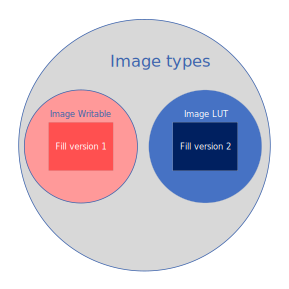
\includegraphics[width=.5\linewidth]{../figures/fill_version_diagram}
%   \caption{Diagram of the two versions of the fill algorithm.}
%   \label{fig:fill.version.diagram}
% \end{figure}


There really are two distinct ways of implementing a basic image algorithm such as \texttt{fill}. For the set of images
type whose values are encoded into each pixel, one must traverse the image and set each pixel's color to the new one.
However, for the set of images type whose data type is encoded in a look-up table, one only has to traverse the look-up
table to set each color to the new one. This translates into two distinct algorithms shown
in~\cref{fig:traverse.vs.LUT}. We can represent the diagram outlining that those two algorithms are two distinct
versions in~\cref{fig:image.version.vs.specialization}.

\begin{figure}[htbp]
  \centering
  \subfloat[Writable image fill algorithm]{
    \(fill(I, v)\colon \forall{p}\in\mathcal{D}, I(p) = v\)
  }
  \hfil
  \subfloat[Image LUT fill algorithm]{
    \(fill(I, v)\colon \forall{i}\in I.LUT, i = v\)
  }

  \caption{Comparison of implementation of the \texttt{fill} algorithm for two
    families of image type.}
  \label{fig:traverse.vs.LUT}
\end{figure}

More generally, we consider that the set of image type is formed of several subsets of image types. In the example there
are two subsets: images whose pixels are writable and images whose values are ordered in a look-up table. \emph{For each
  one of these subsets, if there is a way to implement an algorithm then we have a \emph{version} of this algorithm}.

Sometimes, it is possible to take advantage of a property on a particular image set that may be correlated to an
external data to write the algorithm in a more efficient way. When those properties are linked to the types, it is
called an algorithm \emph{specialization}~\parencite{jarvi.2006.specialization-article}. For instance, when considering
a dilation algorithm, if the structuring element (typically the disc) is decomposable then we can branch on an algorithm
taking advantage of this opportunity: decompose the disc into small vectors (radial
decomposition~\parencite{adams.1993.radialdecomp} or periodic line decomposition~\parencite{jones.1996.periodiclines})
and apply each one of them on the image through multiple passes. The speed-up comparing to a single pass with a large
disc is really significant (illustrated in~\cref{fig:gen.bench.disc.decomp.vs.nodecomp}). The code
in~\cref{fig:dilation.specialization.alg.diagram} illustrate how an algorithm can be written to take advantage of the
structuring element's decomposability property. The algorithm will first decompose the structuring element into smaller
1D periodic lines. It will then recursively call itself with those lines to do the multi-pass and thanks to known
optimizations on periodic lines~\parencite{vanherk.1992.localminmax}, it will be much faster. The dispatch diagram
outlining the different specialization of the dilation algorithm used is show alongside
in~\cref{fig:dilation.specialization.alg.diagram}.

\begin{figure}[htb]
  \centering
  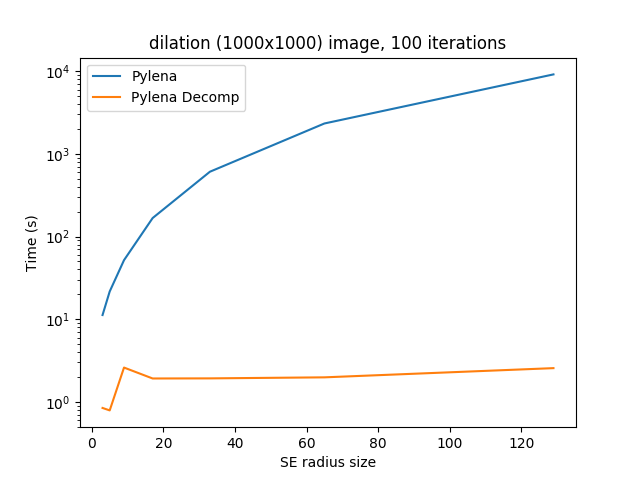
\includegraphics[width=3.8in]{../figures/DilationPln_SEDisc_Benchmarks__Time_vs_SE_size}
  \caption{Benchmark: dilation of a 2D image (\(1000 \times 1000\)) with a 2D disc (decomposable vs. non decomposable).}
  \label{fig:gen.bench.disc.decomp.vs.nodecomp}
\end{figure}


\begin{figure}[htbp]
  \begin{minipage}[l]{0.48\linewidth}
    \begin{minted}{C++}
template <Image Img, StructuringElement SE>
auto dilate(Img img, SE se) {
  if (se.is_decomposable()) {
    lst_small_se = se.decompose();
    for (auto small_se : lst_small_se)
      img = dilate(img, small_se) // Recursive call
    return img;
  } else if (is_pediodic_line(se))
    return fast_dilate1d(img, se) // Van Herk's algorithm;
  else
    return dilate_normal(img, se) // Classic algorithm;
}
\end{minted}
  \end{minipage}
  \hfill
  \begin{minipage}[r]{0.48\linewidth}
    \centering
    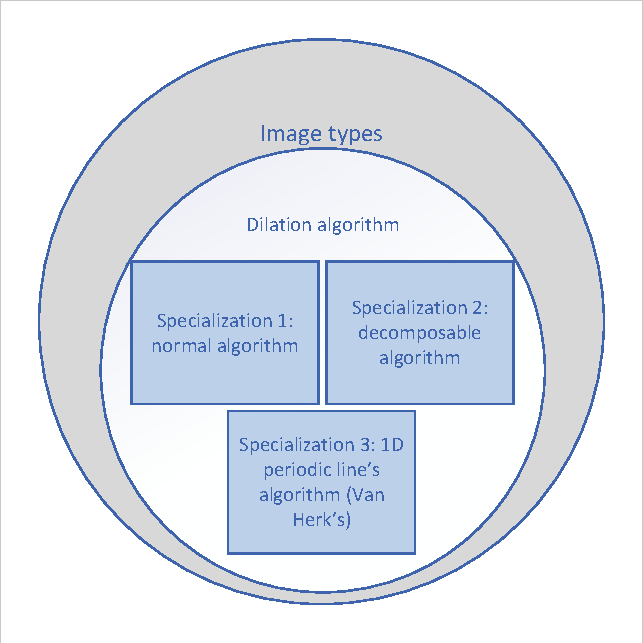
\includegraphics[scale=0.5]{../figures/dilation_specialization_diagram}
  \end{minipage}
  \caption{Dilate algorithm (left) with decomposable structuring element and its specialization diagram (right).}
  \label{fig:dilation.specialization.alg.diagram}
\end{figure}

The~\cref{fig:image.version.vs.specialization} shows how an algorithm specialization may exist in a set of algorithms
version. There exists a specialization of algorithms when the data buffer is known to have the following property: its
memory is contiguous. This implies that, for example, an algorithm like \texttt{fill} can be implemented using low level
and fast primitives such as \texttt{memset} to increase its efficiency.

\begin{figure}[htbp]
  \centering
  \subfloat[Different versions of \emph{fill} algorithm]{
    \includegraphics[width=1.9in]{../figures/image_version}
  }%
  \hfil
  \subfloat[Specialization existing within a version]{
    \includegraphics[width=2.9in]{../figures/image_version_specialization}
  }%
  \caption{Set of algorithm version (a) and its specialization existing within a version (b).}
  \label{fig:image.version.vs.specialization}
\end{figure}

Making a full inventory of image types is not possible as there are many families of image types, each family may
intersect with each other, images may have some particular properties at some points, those properties may appear across
several families of image types. We can nonetheless cite a few to illustrate our points. There exists image types whose
values are cubical complexes~\parencite{ziou.2002.cubical-complex} or layered as hexagonal or triangular grid instead of
square grids (such as meshes), that are represented as graphs~\parencite{meyer.2009.ismm}, etc. All of those interleaves
with different research areas (computer vision for meshes, topological classification for complex
cells~\parencite{movn.20.cviu,allili.2001.cubical}, graph theory and hierarchy for image
graphs~\parencite{carlinet.2014.tip,carlinet.2015.tip,perret.2019.higra}). Finally, this image type inventory does not
help when it comes to designing an image processing library. Instead, what helps is making an inventory of image
processing algorithms as well as what properties those algorithms can leverage to speed up their execution.

Therefore, making the inventory of image processing algorithms (limited to mathematical morphology) outlines three main
families of image processing algorithms. The first one regroups the pixel-wise algorithms. Those algorithms are the
basic pixel-wise transformation. They are the base of any image processing toolkit. Indeed, being able to extract the
green or red color channel of an image is mandatory. Thresholding as well as the previously seen gamma correction
belongs to this family. The second one regroups the local algorithms. Those algorithms perform transformations by
considering all the neighboring pixels around a given pixel. Those algorithms need additional data in the form of an
image's extension (to define border's behavior) and a structuring element (disc, rectangle around the considered pixel).
Such algorithms are widely used in mathematical morphology. Dilation, erosion, closing, opening, gradient, rank filter
are all local algorithms, as well as stencil-type algorithms such as union-find, max-tree or skeletonize. Finally, the
third family regroups the global image processing algorithms. This set contains algorithms where computing the current
pixel requires to knowledge about what was previously computed for the previous pixels. Chamfer distance transform,
labeling, watershed, hierarchy structures related algorithms belongs to this category.


\section{Generic aspect of algorithm: canvas}
\label{sec:canvas}

Genericity is always referred to with this sentence \blockquote{write once, work for every type, run everywhere}.
However, very quickly we learned that the \emph{run} aspect can be a combination of:
\begin{itemize}
  \item as fast as possible on a single CPU unit;
  \item as fast as possible by using many CPU units;
  \item as fast as possible by using many GPU units;
  \item as fast as possible by using many computers (cloud) and their CPU/GPU units.
\end{itemize}
How do we decide what is the most efficient way to do? There is no simple answer to this question, but we can start by
studying the computational shape of algorithms with two goals in mind: (i) find what can be parallelized/distributed and
(ii) find one or several algorithms' abstraction. Indeed, in image processing there are a lot of common patterns when
one looks at algorithms implementations, the most famous being \emph{for all pixels of an image, do something to each
  pixel}. But there are other more high-level similarities that we can leverage to have more generic algorithm. Let us
first study the different programmatic models there are commonly used to process images.

\paragraph{The pipeline} This old and proven model is especially useful to do pre-processing and post-processing
routines. It is a very robust way of structuring a workflow. It consists in an imbrication of different operators
(algorithms) taking as input one or several images, maybe additional data (such as labels, adjacency map, etc.) in order
to process the data int a \blockquote{left-to-right} order. The result will show at the end of the pipeline and the
optimization opportunities are located inside the smaller operators and in the form of correctly managing data (no
unnecessary data copy, locality, etc.)

\paragraph{Kernels and tiling} This programmatic model is engineered to leverage the massive resources available on GPU.
This is the trendy way of the last decade. It consists in breaking the original image into small tiles, and then to feed
those tiles into a massively multicore GPU (via CUDA, Halide~\parencite{ragankelley.2013.halide}). Processing will
happen concurrently on those core, but it is costly to swap contents inside those GPU from the RAM memory. It's then
preferred to design pipeline for those tiles so that the work directly happens on each core to minimize the number of
back and forth copies from the RAM.

\paragraph{Cloud computing} It is a huge deal in image processing these last years as well, especially used in Deep
learning applications. Deep neural networks are usually executed on cluster of computer through network (cloud) and thus
are leveraging combinations of successive \emph{MapReduce}~\parencite{dean.2008.mapreduce} under the hood. Deep learning
frameworks (such as Tensorflow/Keras~\parencite{tensorflow.2015.whitepaper,chollet.2015.keras,gulli.2017.deep},
PyTorch~\parencite{paszke.2019.pytorch}, etc.) take care of offloading work locally (CPU multithreading, GPU kernels and
tiling) while cloud provider infrastructures (such as Azure, AWS) dispatch the top level tasks on their clusters.

\bigskip

In every case there is a notion of pipeline where the user pipe algorithms into each others in order to achieve a
result. Those algorithms can leverage all the heterogeneous resources (cloud, GPU, CPU) available to \emph{map} the
input data. Algorithms will then finally aggregate the results (\emph{reduce}) to output them into another algorithm, or
save them, or display them. It is important to dissociate the route the data will go through and the processing pipeline
logic. Both have their own specificities. In this thesis, we make a parallel, at small scale, between processing
pipeline logic and image processing algorithms. First let us study two basic algorithms: dilation and erosion. The
Python code for those algorithms is naively given in~\cref{code:erode.dilate}.

\begin{figure}[htbp]
  \centering
  \subfloat[Dilation]{
    \includegraphics[width=1.7in]{../figures/dilation_code}
  }%
  \hfil
  \subfloat[Erosion]{
    \includegraphics[width=1.7in]{../figures/erosion_code}
  }%
  \caption{Dilate and Erode algorithms.}
  \label{code:erode.dilate}
\end{figure}

The algorithms are almost written the same way. The only change is the operation \emph{min} and \emph{max} when
selecting the value to keep. As such, we can easily see a way to factorize code by passing the supremum operator as a
function parameter. The algorithms can then be rewritten as shown in~\cref{code:erode.dilate.factorized}. In this last
example, we have one piece of code which is in charge of abstracting the way an image is traversed: we name it the
\emph{canvas}. We also have other pieces of code which carry the logic of the operations, calling the canvas and
providing the logic to apply from within the canvas. This way of decomposing the code offers the opportunity of writing
more specific heterogeneous logic for the traversing code so that the other parts of the code that carry the high-level
logic remains unaware and unburdened of possible implementation details.

\begin{figure}[htbp]
  \centering
  \subfloat[Local algorithm with custom operator]{
    \includegraphics[width=3.28in]{../figures/local_op_code}
  }%
  \vfil
  \smallskip
  \subfloat[Dilation (delegated)]{
    \includegraphics[width=1.64in]{../figures/local_op_dilation_code}
  }%
  \hfil
  \subfloat[Erosion (delegated)]{
    \includegraphics[width=1.64in]{../figures/local_op_erosion_code}
  }%
  \caption{New Dilate and Erode algorithms.}
  \label{code:erode.dilate.factorized}
\end{figure}

\subsection{Taxonomy and canvas}
\label{subsec.taxonomy.canvas}

This approach is very much compatible with the inventory of the algorithms we did in the previous~\cref{sec:image.set}.
Indeed, for the point-wise family of algorithms, it is hardly an issue as they can all be written in terms of views
(cf.~\cref{chap:image_views}). For the second family that consists in all the local algorithm, they can be abstracted
behind an algorithm canvas where the user provides the task to perform for each point of the algorithm. For instance, a
single pass local algorithm will always have shape given in~\cref{code:local.algorithm.canvas}. Finally, for the third
family which consists in all the algorithm that propagate their computation while traversing the image. There is no
trivial way to provide an algorithmic canvas as each algorithm has its own way to propagate changes curing its
computation.

\begin{figure}[htbp]
  \centering
  \begin{minted}[linenos,xleftmargin=17pt,gobble=2]{python}
  def local_canvas(img, out, se):
    # do something before outer loop
    for pnt in img.points():
      # do something before inner loop
      for nx in se(pnt):
        # do something inner loop
      # do something after inner loop
    # do something after outer loop
  \end{minted}

  \caption{Local algorithm canvas.}
  \label{code:local.algorithm.canvas}
\end{figure}

The canvas at~\cref{code:local.algorithm.canvas} can be customized to do a specific job, especially at the lines 2, 4,
6, 7 and 8. The user would then provide callbacks and the canvas would perform the tasks. This is especially useful when
knowing that the canvas can handle the border management (the user would only need to provide a handling strategy like
mirroring the image or filling the border with a value). The canvas can also take advantage of optimization
opportunities (such as decomposing a structuring element) that the user would probably forget, or not know, when first
writing his local algorithm. Another advantage is the opportunity to do more complex optimization such as parallelizing
the execution or offloading part of the calculation on a GPU. More generally, all optimization done through
heterogeneous computing would be available by default even if the user is not a field expert.

Despite all these advantages, one big disadvantage is the readability of the algorithm user-side. For instance, the
dilation algorithm leveraging the local canvas is rewritten in~\cref{code:local.algorithm.dilate}.

\begin{figure}[htbp]
  \centering
  \begin{minted}{python}
def dilate(img, out, se):
  do_nothing = lambda *args, **kwargs: None

  def before_inner_loop(img, out, pnt):
    out(pnt) = img(pnt)

  def inner_loop(ipix, opix, nx):
    out(pnt) = max(out(pnt), img(nx))

  local_canvas(img, out, se,
    before_outer_loop = do_nothing,
    before_inner_loop = before_inner_loop,
    inner_loop        = inner_loop,
    after_inner_loop  = do_nothing,
    after_outer_loop  = do_nothing
  )
  \end{minted}

  \caption{Dilation using the local algorithm canvas.}
  \label{code:local.algorithm.dilate}
\end{figure}

This way of thinking algorithms is far less readable than the classic way. The user does not see the loops happening,
and it can become very messy when several passes are happening (closing, opening, hit or miss, etc.)


\subsection{Heterogeneous computing: a partial solution, canvas}
\label{subsec:heterogeneous}

One of the key aspect driving genericity is performance. We still have the following mantra: \blockquote{write once,
  work for every type, run everywhere}. However, when considering the \emph{run} aspect, there is a lot to do. Indeed,
nowadays, leveraging the available resources to their maximum is long-standing issue. There are many ongoing works on
the subject, such as SyCL~\parencite{brown.2019.heterogeneous,wong.2019.heterogeneous} which is a standard for
heterogeneous computing model edited by Kronos. This standard currently has four implementations: Codeplay's
ComputeCpp~\parencite{codeplay.2021.computecpp}, Intel's LLVM/clang implementation~\parencite{intel-llvm.2021.sycl},
triSYCL~\parencite{xilinx.2021.triSYCL} led by Xilinx and hipSYCL~\parencite{aksel.2020.hipsycl} led by Heidelberg
University. There also exists smaller libraries such as Boost.SIMD~\parencite{esterie.2014.boostsimd} or even
VCL~\parencite{fog.2013.vcl} to ease writing SIMD code. After taking some distance to study the subject, we can infer
that there are three main aspects to consider when optimizing performance.

The first one, the most important one is the algorithm to use in accordance with the set of data. This aspect is covered
by the C++ language and its built-in genericity tool: template metaprogramming. Indeed, we can select the most suitable
algorithm for a particular set of data.

The second one is the ability for the code to be understood by the compiler so that it can be further optimized during
the generation of the binary. Indeed, when compiling for the native architecture of a recent processor, the compiler can
use the most recent assembly instructions to use wide vectorized registries (AVX512). The use of an up-to-date compiler
infrastructure also brings the help much needed.

Finally, the third aspect is not as trivial as the first two ones. It consists in studying the structure of an algorithm
to allow distributed computation. It also consists in studying the different architectures to select the most efficient
algorithm for each particular architecture. Sometimes algorithm are friendly to their distribution on several processing
units that compute a part of the result concurrently. This is what we call parallelism. There exists several ways to
take advantage of parallelism. First there is the use of several CPU units on the host computer. Then there is the use
of GPU units working in combination with the CPU units to take advantage of the massive amount of core a graphic card
can provide. Finally, there is the use of cloud computing which consists in using several ``virtual'' computers, each of
them offering CPU and GPU units available to compute a result. However, each time we introduce a new layer of
abstraction, there is a cost to orchestrate the computation, send the input data and retrieve the results. Therefore, it
is very important to study case by case what is needed. Some solutions exist to abstract away completely the hardware
through a DSL~\footnote{Domain Specific Language} such as Halide~\parencite{ragankelley.2013.halide}: the DSL compiler's
job will be to try very hard to make the most out of both the available (or targeted) code and hardware. Those solutions
are not satisfactory for us as we want to avoid using a DSL to remain at code level (core language only). We are not
developing a compiler: we are working with it.

There is one true issue when studying parallel algorithms: it is whether they can be parallelized or not. Not all
algorithms can be parallelized. Some just intrinsically cannot, typically, algorithms that immediately need the result
of the previous iteration to compute the next iteration. There may exist specific ways to re-arrange a specific
algorithm, for instance, taking advantage of some algebraic property, in order to rewrite it in a parallelizable way,
but it is not trivial (it is done on a per-algorithm basis), and not generic. As such, it is out of the scope of this
thesis. What interests us are the algorithms whose structure is an accumulation over a data type that can be defined as
a monoid. We assert that every algorithm that can be rewritten as an accumulation over a monoid can be parallelized
and/or distributed. This model, that consists in distributing computation like an accumulation over a monoid data
structure, is also call the ``\emph{map-reduce}''. This model has two steps: the distribution (map) and then the
accumulation (reduce).

The \emph{map} step dispatches computation on subunits with small set of data. The \emph{reduce} step retrieves and
accumulate all the results' data as soon as they are ready.

The accumulation algorithm has this shape:
\begin{minted}[linenos]{C++}
  template <class In, class T, class Op>
  auto accumulate(In input, T init, Op op)
  {
    for(auto e : input)
    {
      init = op(init, e);
    }
    return init;
  }
\end{minted}

The loop line 4 can be split into several calculation units which are going to be distributed, and then accumulated
later once the units have finished their computation.

The issue left here is the monoid. What exactly is a monoid here? A monoid is a data structure which operates over a set
of values, finite or infinite. This data structure must provide a binary operation which is closed and associative.
Finally, this data structure must also provide a neutral element (aka the identity). Some trivial monoids comes to mind:
\begin{itemize}
  \item \emph{boolean}. For binary operation ``and'', identity is ``true'' whereas for binary operation ``or'', identity
        is ``false''.
  \item \emph{integer}. For binary operation \(-\) and \(+\), identity is \(0\) whereas for binary operation \(*\) and
        \(/\), identity is \(1\).
  \item \emph{string}. For concatenation, identity is empty string.
  \item \emph{optional} value (also known as monadic structure in Haskell programming language).
\end{itemize}
There are many more monoids, less trivial but very handy, such as the unsigned integer/max/0 set and the signed
integer/min/global max set.

This theory is extremely beneficial to image processing as the most commonly used algorithms, the local algorithms, can
all be written in the form of an accumulation over the pixels of an image. The fact that finding an identity for the
operation processed by the algorithm is often quite trivial led us to the idea of canvas. A canvas is a standard way to
write an iteration over an image which abstracts the underlying data structure. A canvas is a tool for the user to
provide its computation model based on events such as: \blockquote{entering inner loop} or \blockquote{exiting inner
  loop}. The user can then provide its operations as if he was writing his algorithm himself (restricted to the
accumulation model). As the maintainer of the library provides the canvas of execution, he can know also make change to
take advantage of it. For instance, computing a CUDA kernel at one point and dispatching it on GPU units is totally
within scope and remains transparent for the user of the library. Although there is a caveat: rewriting our algorithm in
an accumulation shape and chunking it in fragments to feed to the canvas is definitely not intuitive. Indeed, we require
our user to change his way of thinking from the procedural paradigm to the event-driven paradigm. This approach is not
new and is used in other libraries such as Boost.Graph~\parencite{siek.2001.boostgraph} for similar purposes.
\citeauthor{dean.2019.monoids} talks about this recurring monoid pattern more in-depth in his
talk~\parencite{dean.2019.monoids}.

In image processing, we quickly identify \emph{local} algorithms. They reason about a group of pixel around a given of
coordinate. All those algorithms can be abstracted behind an accumulation of some sort, and they all have the same
morphology. Thus leading to the following abstraction:
\begin{minted}{C++}
template <class In, class Out, class SE, class T, class Op>
auto local_accumulate(In input, Out output, SE se, T init, Op op)
{
    auto zipped_imgs = ranges::view::zip(input.pixels(), output.pixels())
                                                  // (1)
    for(auto&& rows : ranges::rows(zipped_imgs))
    for(auto [px_in, px_out] : rows)
    {
        auto v = op(init, px_in.val());           // (2)
        for(auto nb : se(px_in))
        v = op(v, nb.val());                      // (3)
        px_out.val() = v;                         // (4)
      }
                                                  // (5)
  }
\end{minted}
From this code we can deduce some very useful and easy monoids by the following triplets:
\begin{itemize}
  \item \((type = boolean, operator = and, neutral = true)\) is a binary erosion
  \item \((type = boolean, operator = or, neutral = false)\) is a binary dilation
  \item \((type = unsigned\ integer, operator = max, neutral = 0)\) is a dilation
  \item \((type = signed\ integer, operator = min, neutral = global max)\) is an erosion
\end{itemize}

Now if we want to rewrite the \texttt{local\_accumulate} in an event driven paradigm, we need to identify the different
callbacks to expose to our user on the call site. Especially, what will be the callback parameters. There are five
callback events that we have identified:
\begin{enumerate}
  \item before entering outer loop (no work is done)
  \item before entering inner loop (iteration over the pixel's neighbor)
  \item inner loop (actual operation to perform, result is accumulated)
  \item after exiting inner loop (iteration over the neighbor is over, what to do with the accumulated result?)
  \item after exiting outer loop (iteration over the image is over)
\end{enumerate}
\begin{minted}{C++}
template <class In, class Out, class SE, class T, class BeforeOuterLoopCB,
          class BeforeInnerLoopCB, class InnerLoopCB class AfterInnerLoopCB,
          class AfterOuterLoopCB>
auto local_accumulate(In input, Out output, SE se, T init,
                      BeforeOuterLoopCB bolCB, BeforeInnerLoopCB bilCB,
                      InnerLoopCB ilCB, AfterInnerLoopCB ailCB,
                      AfterOuterLoopCB aolCB)
{
  auto zipped_imgs = ranges::view::zip(input.pixels(), output.pixels()
  bolCB(input, output);                             // (1)
  for(auto&& row : ranges::rows(zipped_imgs))
    for(auto [px_in, px_out] : rows)
    {
      bilCB(px_out.val(), init, px_in.val())        // (2)
      for(auto nb : se(px_in))
        ilCB(px_out.val(), px_out.val(), nb.val())  // (3)
      ailCB(px_out.val(), init, px_in.val())        // (4)
    }
  aolCB(input, output)                              // (5)
}
\end{minted}
In this code, we can see that all the callbacks do not take the same type and/or number of parameters. Here is what the
call site could look like if the user wants to perform a dilation:
\begin{minted}{C++}
local_accumulation(
  input,                                    // input image
  output,                                   // output image
  se,                                       // structuring element
  0,                                        // monoid's neutral element
  [](auto I, auto& O) { /* do nothing */ }, // (1) entering outer loop callback
  [](auto& o, auto init, auto in){          // (2) entering inner loop callback:
    o = std::max(init, in);                 // initialize with neutral element
  },
  [](auto& o, auto cur, auto nbh) {         // (3) inner loop callback:
    o = std::max(cur, nbh);                 // keep the local maximum
  },
  [](auto& o, auto init, auto in) {         // (4) exiting inner loop callback
    /* do nothing */
  },
  [](auto I, auto& O) { /* do nothing */ }  // (5) exiting outer loop callback
);
\end{minted}
It is very verbose and non-intuitive but hopefully, once the compiler optimize out the empty callbacks, the generated
code is as fast as a non-generic handwritten dilation.

\section{Library concepts: listing and explanation}
\label{sec:library.concepts}

Let us now delve into the concepts related to the Image Processing area. Indeed, this domain has his specificities, and
we want to improve generic image processing library design by learning from our past experiments and by working with new
techniques. The most basic usage of an image is the famous algebraic formula \(y = f(x)\) where \(y\) is a \emph{value}
generated by the \emph{image} \(f\) for the \emph{input} \(x\). Aside from generating a value, an image can also
\emph{store} a value, as in \(f(x) = y\) where the value is \emph{assigned} to the image for a given point. Those
notions are the basis of our work and will drive the entire design.

\subsection{The fundamentals}

\label{subsec:fundamentals}

First, let us introduce the fundamental concepts deriving from the basis notion. The \emph{Value} concept is refined
into three distinct one (details in~\cref{table:concept.value.expressions}). There are the basic \emph{Value} but also
the \emph{ComparableValue} and the \emph{OrderedValue} which are useful when it comes to comparison or ordering
algorithms. The need behind those three concepts derives from the algorithms which require an ordering relation in order
to function properly. Most of mathematical morphology algorithms requires it. For instance, the ordering relation for a
gray-scale image is trivial whereas it is a field of research for colored (rgb 8-bits) images.

The second fundamental brick is the concept of \emph{Point}, detailed in~\cref{table:concept.point.expressions} which is
a bit less open than the concept \emph{Value} as it must be totally ordered. Indeed, when it comes to accessing a value
stored in an image, whether it is for reading or for mutating purpose, it is important that there is exactly one value
accessed.

We Now introduce an abstract way to represent this relation \(Value \times Point\): the \emph{Pixel}. This is a well
known notion in image processing, and it represents a couple \((point, value)\). This abstraction layer is easy to move
around and contains facilities to read and mutate the pixel's value if possible. Indeed, not all pixels can mutate their
value. If the pixel is yielded by an image that only generates values on the fly then it cannot mutate it. Henceforth,
we introduce two new concepts: \emph{Pixel} and \emph{OutputPixel} (details in~\cref{table:concept.pixel.definitions}).
Those two concepts have a very similar interface described in~\cref{table:concept.pixel.expressions}. They can both
access the stored information: the point and the value. On top of that, the \emph{OutputPixel} can mutate its value.
When interacting with pixels, the user is able to write code as followed:
\begin{minted}{C++}
  auto pix = Pixel();     // Get a pixel
  auto val = pix.val();   // yield the pixel value
  auto pnt = pix.point(); // yield the pixel point
  pix.val() = 42;         // Assign a value
\end{minted}

We show how those three fundamental concepts interact with each other in the\\
diagram~\cref{fig:concept.pixel}.

\begin{figure}[htbp]
  \centering
  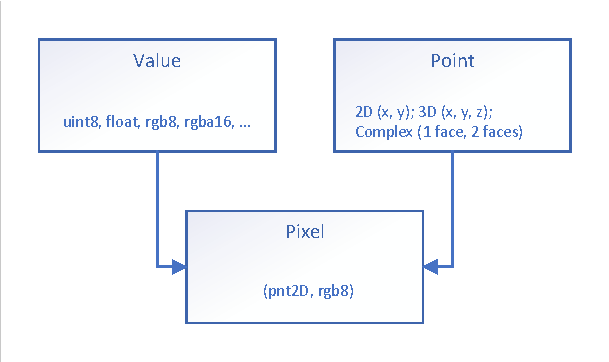
\includegraphics[width=.8\linewidth]{../figures/concepts/pixel}
  \caption{Pixel concept.}
  \label{fig:concept.pixel}
\end{figure}

Now we need a helper concept: the \emph{ranges}.
Ranges~\parencite{niebler.2014.ranges,niebler.2018.ranges,niebler.2018.deepranges,niebler.2018.mergingranges} are a set
of concepts defined in the C++ standard library shipped with the ISO C++20 norm in 2020~\parencite{iso.2020.cpp}. They
allow the user to abstract away iterators so that the iteration occurs directly over the values. This offers the user
the opportunity to migrate his source code from being:
\begin{minted}{C++}
template <class IteratorBegin, class IteratorEnd>
void my_algorithm(IteratorBegin beg, IteratorEnd end)
{
  for(; beg != end; ++beg)
    // use *beg to access the value
}
\end{minted}
To being:
\begin{minted}{C++}
template <class Range>
void my_algorithm(Range rng)
{
  for(auto&& val : rng)
    // use val  to access the value
}
\end{minted}

In image processing, we refine further this concept by introducing multidimensional ranges (\emph{MDRange}). Indeed, in
image processing the user is used to write double loop to iterate over a bi-dimensional image. Abstracting away this
aspect under standard ranges induces performance loss. That is why we need to introduce this additional concept. A
multidimensional range can be split with a library function, \texttt{mln::ranges::rows(mdrng)} to fit the double-loop
pattern while retaining high performances. This topic is tackled in-depth later in~\cref{subsec.range.traversing}. For
now, let us consider multidimensional ranges as an image processing extension for performance for the image traversing
pattern. They are defined in~\cref{table:concept.ranges.definitions} and their interface is the same as standard ranges,
as seen in~\cref{table:concept.ranges.expressions}. They are designed so that the user code can look like this:
\begin{minted}{C++}
  auto mdrng = MDRange(); // Get a multi-dimensional range of values
  auto rows = mln::ranges::rows(mdrng);
  for(auto row : rows) // double loop pattern
    for(auto val : row)
      // use(val)
\end{minted}

From an algebraic point of view, the definition of an image is not complete without considering a definition domain on
which it is defined. In image processing, the same rule applies. We cannot consider an image without considering the set
of points that are valid for this image. Henceforth, we must define the concept of \emph{Domain} (details
in~\cref{table:concept.domain.definitions}). The \emph{Domain} concept is refined into two sub-concepts named
\emph{SizedDomain} and \emph{ShapedDomain}. This makes the existence of infinite domain and domains that may be defined
over non-continuous intervals in space possible. This enables algorithms to require the domain to have certain shape if
needed. The domain behavior is described in~\cref{table:concept.domain.expressions}.

In practice, a domain is used to get information about the points constituting the image. Indeed, we can write code
like this:
\begin{minted}{C++}
  auto dom = Domain(); // Get a domain
  auto pnt = Point(..., ...); // Get a random point
  bool ret = dom.has(pnt); // Check wether the domain contains the point
  bool is_empty = dom.empty(); // Check wether the domain is empty
  auto dim = dom.dim(); // Yield the domain's dimension information
  for(auto pnt : dom) // browse the definition domain
    // use pnt as a point of the domain
\end{minted}

We show how the concept \emph{Domain} flows from the previous concepts in the diagram shown in~\cref{fig:concept.domain}.

\begin{figure}[htbp]
  \centering
  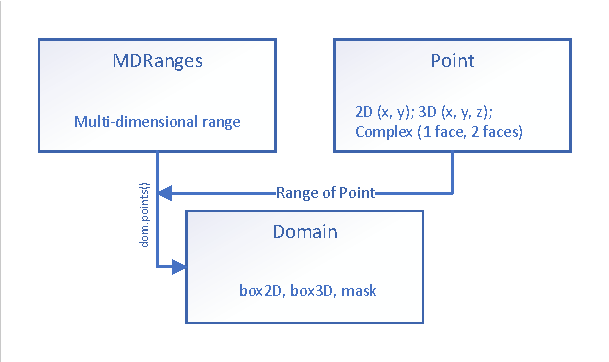
\includegraphics[width=.8\linewidth]{../figures/concepts/domain}
  \caption{Domain concept.}
  \label{fig:concept.domain}
\end{figure}

All the prerequisites to introduce our main concept: \emph{Image} are fulfilled. Similar to \emph{Pixel}, we have the
distinction over image whose value can be mutated in a sub-concept named \emph{WritableImage}. These concepts are
defined in~\cref{table:concept.image.definitions.1}. In addition to this definition, we can infer the behavior described
in~\cref{table:concept.image.expressions.1}. There are complicated requirements written in template metaprogramming code
and, in summary, they just require that the value types of the ranges returned by the member functions \texttt{pixels()}
and \texttt{values()} are the same as the value types declared in the parent image type. In addition, we introduce two
facilities which are the member function \texttt{concretize()} and \texttt{ch\_value<V>()}. The first is a way to turn a
view into a concrete type. This will be seen more in-depth in~\cref{chap:image_views}. The last is a way to cast values
from one type to another. It forms a new image type whose underlying values will be returned after being converted to a
new value type. This last facility is extremely useful when we only want to cast the underlying type while keeping all
the other details (such as the dimension) identical. For instance, when working with labeling algorithm, we know our
algorithm will return an image similar to the input one except for the underlying type which will be the type of the
label. The following code shows how it is used:
\begin{minted}{C++}
  using label_t = int; // label type

  template <class I> // Input image of type I
  auto my_labeling_algorithm(I input_image)
    -> image_ch_value_t<I, label_t> // Output image is Input image (I)
                                    // whose underlying type is label_t
  {
    // ...
  }
\end{minted}

We show the diagram building up the image concept from the previous concepts in~\cref{fig:concept.image}.

\begin{figure}[htbp]
  \centering
  \includegraphics[width=.99\linewidth]{../figures/concepts/image}
  \caption{Image concept.}
  \label{fig:concept.image}
\end{figure}


\subsection{Advanced way to access image data}
\label{subsec:advanced}

While being able to iterate over ranges of pixels or values is good, we are still lacking fundamental facilities to
access an element directly from the image. In order to solve this predicament, first we need to define the concept of
\emph{Index} in~\cref{table:concept.index.expressions} which we will use afterwards. This is a very simple concept that
encapsulate an integral value. This value can be negative as we want to be able to do negative indexing in case our
image has an extension, cf.~\cref{subsec:advanced}. The first advanced concept is represented as an
\emph{IndexableImage}. An element can be accessed simply by providing its index number. This concept is defined
in~\cref{table:concept.image.definitions.2}. This introduces a simple behavioral pattern described
in~\cref{table:concept.image.expressions.2}. With this concept, we are able to write code as followed:
\begin{minted}{C++}
  auto ima = IndexableImage(); // Get an indexable image
  int k = 15; // Get an index
  auto val = ima[k]; // Get the element at the index
  ima[k] = 255; // Mutates the element at the index
\end{minted}
Being able to traverse an image through indexes is especially useful for algorithms that are aware of the number of
elements in the image. We chose to be flexible with our indexing method (i.e. allowing signed indexes) not to fall into
the same pitfall as the C++ standard library~\parencite{stroustrup.2019.signed-unsigned-mess}. Indeed, requiring that
the standard type \texttt{std::size\_t} is unsigned led to loads of issues, the first one being a conversion issue when
writing a simple for-loop. Solving these issues led to the appearance of new member function \texttt{.ssize()} (for
signed size) and the new standard type \texttt{std::ptrdiff\_t} to store the result of a subtraction between two
\texttt{std::size\_t}. Furthermore, in our specific area (image processing), it may be well-defined to access a buffer
with negative indexes when, for instance, we are accessing the value of the extension of an image. This is why our
indexes are signed.

Additionally, we want to be able to access a value by providing a point, the same way as in the algebraic definition
\(val = image(point)\). To do so, we introduce the concept of accessibility through \emph{AccessibleImage}. This concept
is defined in~\cref{table:concept.image.definitions.3}. This introduces new behavior that is described
in~\cref{table:concept.image.expressions.3}. We can notice some facilities specifically including bound checking.
Indeed, we suppose, for fast access, that the user is always picking element from the image's domain, but it is possible
to bound check elements if needed on access for specific usages. With this concept, we are now able to write code as
followed:
\begin{minted}{C++}
  auto ima = AccessibleImage(); // Get an accessible image
  auto p = Point(); // Get a point
  auto val = ima(p); // Get a value from a point
  auto val = ima.at(p) // Same with no bound checking
  auto pix = ima.pixel(p) // Get a pixel from a point
  auto pix = ima.pixel_at(p) // Same with no bound checking
  ima(p) = 42; // Assigns a value from a point
  ima.at(p) = 42; // Same with no bound checking
  ima.pixel(p).val() = 42; // Assigns a pixel value from a point
  ima.pixel_at(p).val() = 42; // Same with no bound checking
\end{minted}
Being able to traverse an image with points is especially useful for algorithms relying on restricting/expanding
definition domain that are exclusively yielding points.

Once we know that an image is both \emph{indexable} and \emph{accessible} we can introduce new behaviors (described
in~\cref{table:concept.image.expressions.4}) that we put behind the concept of \emph{IndexableAndAccessibleImage}
defined in~\cref{table:concept.image.definitions.4}. This behavior is related to retrieving an index from points and
vise versa. Indeed, it is now possible to write such code:
\begin{minted}{C++}
  auto pnt = ima.point_at_index(k); // Get the point from an index
  auto k = ima.index_of_point(pnt); // Get the index from a point
  // Get the index difference for a shift of delta_point
  auto delta_idx = ima.delta_index(delta_pnt);
\end{minted}

Additionally, it is useful, for propagating algorithms, to be able to traverse images in both a forward way and a
backward way. As it may not be possible for all images, this notion needs to be refined into a new concept
\emph{BidirectionalImage}. This concept is defined in~\cref{table:concept.image.definitions.5} and its behavior is
described in~\cref{table:concept.image.expressions.5}. Thanks to this concept, we are able to write code as followed:
\begin{minted}{C++}
  template <class I>
  my_algorithm(I input)
  {
    // forward pass
    for(auto pix : input.pixels())
      // use pix

    auto backward = mln::ranges::views::reverse(input.pixels())
    for(auto pix : backward)
      // use pix
  }
\end{minted}

Finally, we need a way, when possible, to iterate over a contiguous data buffer for very fast and optimized calculation.
That is what the concept of \emph{RawImage} is for: an image whose data buffer can be accessed, as well as its mutable
counterpart, which are defined in~\cref{table:concept.image.definitions.6}. Having a raw image whose data buffer can be
accessed enables us to expose two more member functions to access the data buffer and its strides to compute accurate
pointer arithmetic. They behave as described in~\cref{table:concept.image.expressions.6}. This allows writing code as
followed:
\begin{minted}{C++}
  auto ima = Image(); // Image of int
  const int* data = ima.data(); // Access the underlying buffer
  auto dim = ima.domain().dim(); // Get the dimension of the image
  // Retrieve information about strides
  auto strides = std::vector<std::ptrdiff_t>(0, dim)
  for (int i = 0; i < dim; ++i)
    strides[i] = ima.stride(i)

  // Now use data and strides to traverse the raw buffer
  // ...
\end{minted}

We show how those concepts are defined and interact with each other in the diagram shown in~\cref{fig:concept.images}.

\begin{figure}[htbp]
  \centering
  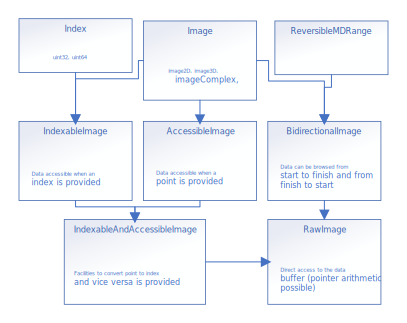
\includegraphics[width=.8\linewidth]{../figures/concepts/images_all}
  \caption{All images concepts.}
  \label{fig:concept.images}
\end{figure}


\subsection{Local algorithm concepts: structuring elements and extensions}
\label{subsec:local.se.ext}

From the beginning concepts emerge from behavioral patterns extracted from algorithms. In image processing, there is a
family of algorithms called the \emph{local algorithms}. They work by considering a specific pixel as well as all the
pixels surrounding within a window that has a specific shape centered in this first pixel. The window is called the
\emph{structuring element} and the pixels considered by this window are called the \emph{neighborhood}. This leads us to
introduce the concept of \emph{StructuringElement} which is defined in~\cref{table:concept.se.definitions}.

This concept is refined into three sub-concepts that are related to properties a structuring element can provide. Those
properties are:
\begin{itemize}
  \item decomposability: ability to split a complex structuring element into several smaller and simpler structuring
        element. There is an equivalence in behavior when the algorithm is recursively run for each smaller structuring
        element one after another, in a multi-pass way.
  \item separability: ability to split a complex structuring element into several smaller and simpler structuring
        element. There is an equivalence in behavior when the convolution is recursively run for each smaller
        structuring element one after another, in a precise order, in a multi-pass way.
  \item incremental: ability to tell the points that are added to or removed from the range when the structuring element
        is shifted by a basic displacement (e.g. for a \emph{2D point}, the basic displacement is \((0,1)\)). Usually
        used to compute attributes over a sliding structuring element in linear time.
\end{itemize}

The~\cref{fig:se.decomp.rect} shows how a $5x5$ rectangle is decomposed into periodic lines.
The~\cref{fig:se.decomp.disc} shows how a disc of radius 3 is decomposed in periodic lines.

\begin{figure}[htbp]
  \centering
  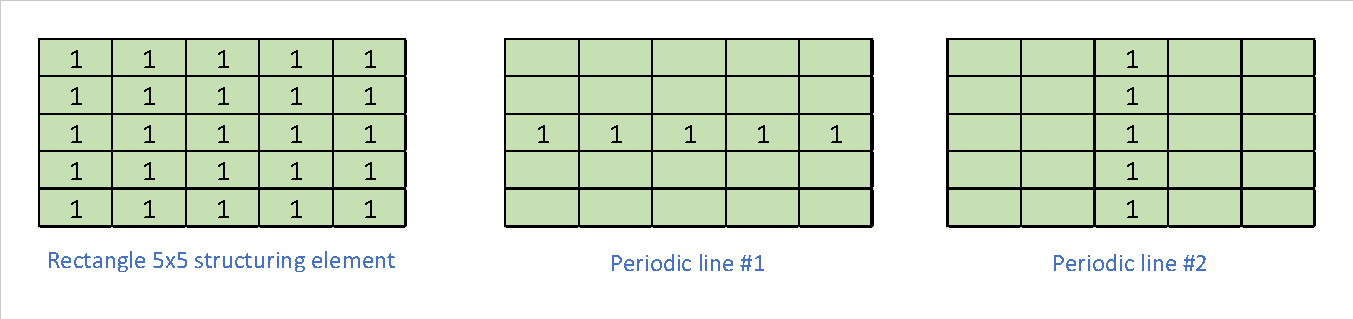
\includegraphics[width=.65\linewidth]{../figures/rect_se_decomp}
  \caption{Decomposition in period lines of a rectangle structuring element.}
  \label{fig:se.decomp.rect}
\end{figure}

\begin{figure}[htbp]
  \centering
  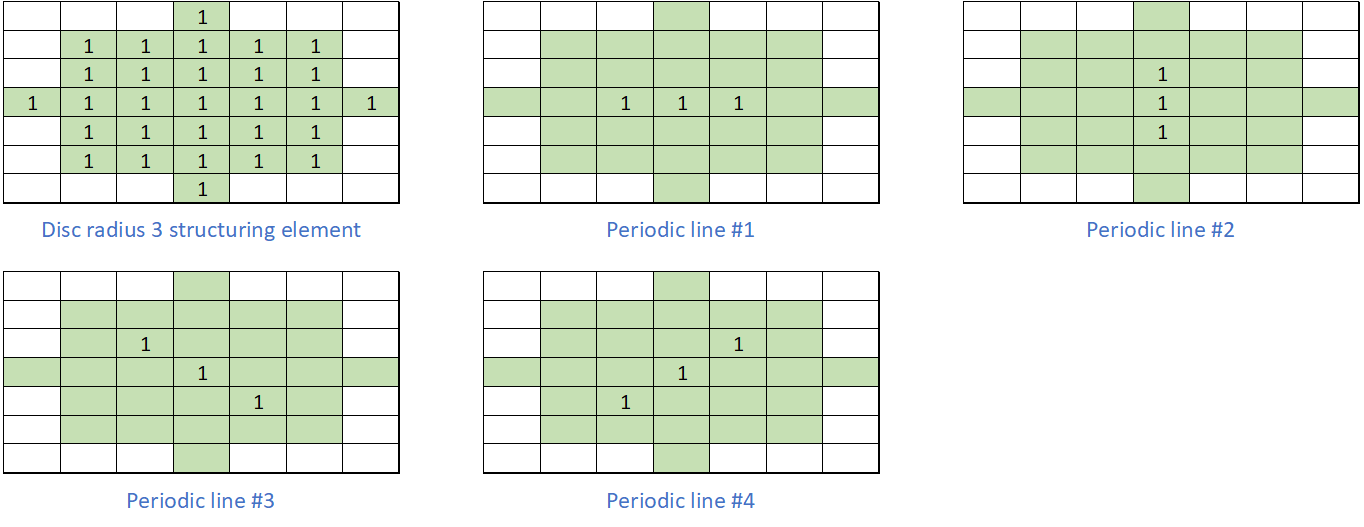
\includegraphics[width=.8\linewidth]{../figures/disc_se_decomp}
  \caption{Decomposition in period lines of a disc structuring element.}
  \label{fig:se.decomp.disc}
\end{figure}

%se::rect2D(pnt2D{2, 2}) :
%
%(0,0) (1,0) (2,0) (3,0) (4,0)
%(0,1) (1,1) (2,1) (3,1) (4,1)
%(0,2) (1,2) (2,2) (3,2) (4,2)
%(0,3) (1,3) (2,3) (3,3) (4,3)
%(0,4) (1,4) (2,4) (3,4) (4,4)
%
%decomposed in periodic lines:
%(0,2) (1,2) (2,2) (3,2) (4,2) 
%(2,0) (2,1) (2,2) (2,3) (2,4) 
%
%incremental
%(4,0) (4,1) (4,2) (4,3) (4,4) 
%
%decremental:
%(-1,0) (-1,1) (-1,2) (-1,3) (-1,4) 
%
%se::disc(radius=3, pnt2d{3, 3}) :
%                  (3,0)
%      (1,1) (2,1) (3,1) (4,1) (5,1)
%      (1,2) (2,2) (3,2) (4,2) (5,2)
%(0,3) (1,3) (2,3) (3,3) (4,3) (5,3) (6,3)
%      (1,4) (2,4) (3,4) (4,4) (5,4)
%      (1,5) (2,5) (3,5) (4,5) (5,5)
%                  (3,6)
%
%decomposed in periodic lines:
%(2,3) (3,3) (4,3) 
%(3,2) (3,3) (3,4) 
%(2,2) (3,3) (4,4) 
%(4,2) (3,3) (2,4) 

The behavior requirements of those concepts is described in~\cref{table:concept.se.expressions}. Being able to
manipulate structuring element allows us to write the following code:
\begin{minted}{C++}
  auto se = se::disc(.radius=3); // get a structuring element
  for(auto pix : ima.pixels())   // traverse image
    for(auto nb : se(pix))       // traverse neighboring pixels
      // ...
\end{minted}

Additionally, we introduce the concept of \emph{Neighborhood} in~\cref{table:concept.nbh.definitions}. This concept has
facilities to know what points/pixels are placed before or after another point/pixel inside the window of a specific
structuring element. It behaves as described in~\cref{table:concept.nbh.expressions}. This concept is useful when one
wants to only consider a certain part of the neighboring pixels within a structuring element. This offers the
opportunity to write the following code:
\begin{minted}{C++}
  auto se = se::disc(.radius=3); // get a structuring element
  for(auto pix : ima.pixels())   // traverse image
    for(auto nb : se.before(pix))// traverse neighboring pixels located before pix
      // ...
\end{minted}

And the last concept we need to introduce is the \emph{extension}. Indeed, extension management is very important when
dealing with local algorithm as pixels on the border need to be processed too. Indeed, the behavior near the border of
the image must be defined and well-specified. There are several strategies when it comes to borders and extension. We
refine a concept for each strategy we have identified:
\begin{itemize}
  \item \emph{fillable}: fill the border with a specific value.
  \item \emph{mirrorable}: mirror the image as if there was an axial symmetry, with the border being the axis.
  \item \emph{periodizeable}: repeat the image, as if a modulo size was applied to the coordinates.
  \item \emph{clampable}: extend the value at the image's border into the extension.
  \item \emph{extent\_with}: used when tiling. It considers the current image as a sub-image of another bigger image and
        pick the extension values from the parent image.
\end{itemize}
Those concepts are defined in~\cref{table:concept.extensions.definitions} and their behavior is described
in~\cref{table:concept.extensions.expressions}. All those concepts allow us to introduce the final refined image
concepts: \emph{WithExtensionImage}, \emph{ConcreteImage} and \emph{ViewImage}. Those two last will be seen in
detail in the next~\cref{chap:image_views}. Those concepts are defined in~\cref{table:concept.image.definitions.7}.
Their behavior is described in~\cref{table:concept.image.expressions.7}. It is now possible to write the following code:
\begin{minted}{C++}
  template <class I, class SE>
  my_local_algorithm(I input, SE se) {
    // if the extension is large enough to function with the passed structuring element
    if(input.extension().fit(se)) {
      // ...
    }
  }
\end{minted}

We show how those three concepts (structuring elements, neighborhood and extension) interact with each other in the
diagram shown in~\cref{fig:concept.se_extension}.

\begin{figure}[htbp]
  \centering
  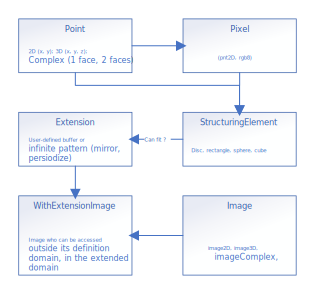
\includegraphics[width=.8\linewidth]{../figures/concepts/se_extension}
  \caption{Structuring element and Extension concepts.}
  \label{fig:concept.se_extension}
\end{figure}

Finally, we introduce a helper concept to centralize the detection of the ``writability'' of an image. Indeed, we do not
want the user to have to use the writable counterpart of each concept for each and every case. That is why we introduce
this final concept, \emph{OutputImage} in~\cref{table:concept.image.expressions.8}, that will tell whether the values of
an image are mutable.

The correct way to use it is:
\begin{minted}{c++}
template <class Img>
requires RawImage<Img> && OutputImage<Img>
void my_algorithm(Img img) {
    // write data in img ...
  }
\end{minted}

\section{Summary}

In this chapter, we present that concepts are not designed after data structures but after algorithms. Indeed, a concept
consists in extracting a consistent behavioral pattern from several pieces of code (algorithms) and name it to give it a
meaning. Through a simple but concrete example, we present in a didactic way to extract concepts from an image
processing algorithm (gamma correction).

This chapter then proceeds to explain how, in theory, image types are related to each other. We present the set of
different image types families and how algorithms exist in those sets, which introduce the notion of \emph{version} of
an algorithm. An algorithm have different \emph{versions} for each image types family it supports. We distinguish it
from an algorithm \emph{specialization}, the latter being the ability to leverage a property to make an optimization and
increase performances.

This chapter then proceeds to describe the notion of algorithm canvas which is the result flowing from the taxonomy of
image processing algorithms. Indeed, there are three main algorithm families: the pixel-wise algorithms (binary
threshold), the local algorithms (dilation) and the global algorithms (Chamfer distance transform). We focus primarily
on local algorithms and how they can all be written with the same canvas of code. Indeed, for instance, the only
difference between a dilation and an erosion is the supremum operator (max vs. min). We then discuss avenues to leverage
these canvas to possibly solve heterogeneous computing issues.

Finally, this chapter introduces our first main contribution: a complete taxonomy related to the image processing area.
We first introduce fundamental concepts such as \emph{point}, \emph{pixel}, \emph{domain} and \emph{image}. We then
motivate and introduce advanced concepts related to images and the different way to access data (forward, backward
traversing, indexing, direct access to underlying buffer, \ldots). In the end, we introduce the concepts related to
orbiting notions such as \emph{structuring element}, \emph{neighborhood} and \emph{extension} (border management) which
are necessary to be able to work with local algorithms.

The next chapter will make use of the presented concepts to introduce the second main contribution of this thesis: the
\emph{image views}.


\cleardoublepage

\chapter{Image views}
\label{chap:image_views}

\lettrine[lines=2]{T}{his} concept of views is not new~\parencite{novak.1997.reuse} and naturally appeared in Image
processing with Milena under the name of \emph{morpher}~\parencite{levillain.2009.ismm,geraud.2012.hdr}. It was always
useful to be able to project an image through a prism that could extract specific information about it without the need
to copy the underlying data buffer. In modern days, the language C++ (20) also introduces this mechanism with the
ranges~\parencite{niebler.2014.ranges} facilities for \emph{non-owning collections}. It is named \emph{views} and allows
the user to access the content of a container (vector, map) through a prism. In Pylene, we decided to align the naming
system after what was decided in C++20 in order not to confuse the user. This way, a \texttt{transform} view in image
processing will do the same thing on an image that the transform view in the standard range library does on a container.
\emph{Views} feature the following properties: \emph{cheap to copy}, \emph{non-owner} (does not \emph{own} any data
buffer), \emph{lazy evaluation} (accessing the value of a pixel may require computations) and \emph{composition}. When
chained, the compiler builds a \emph{tree of expressions} (or \emph{expression template} as used in many scientific
computing libraries such as Eigen~\parencite{guennebaud.2010.eigen}), thus it knows at compile-time the type of the
composition and ensures a 0-overhead at evaluation. We will first motivate the usage of \emph{views} in image
processing. We will then present the main views used in image processing. Then will be discussed how image views differ
from the one used in C++'s ranges and their main properties (especially how they keep/discard the properties from the
parent image) through a concrete example: the management of border and extension policies. Finally, we will discuss the
limitations of such a design.

\section{The Genesis of a new abstraction layers: Views}
\label{sec:genesis_of_views}

In image processing an algorithm is naively written by taking one or several inputs' data (among which is the input
image(s)),  by performing work on this input data and then by returning the resulting data (or an error). Let us take
for example the alpha-blending example which can be implemented in naive C++ code as followed:
\begin{minted}{C++}
  void blend_inplace(const uint8_t* ima1, uint8_t* ima2, float alpha,
  int width, int height, int stride1, int stride2) {
    for (int y = 0; y < height; ++y) {
      const uint8_t* iptr = ima1 + y * stride1;
      uint8_t* optr = ima2 + y * stride2;
      for (int x = 0; x < width; ++x)
        optr[x] = iptr[x] * alpha + optr[x] * (1-alpha);
    }
  }
\end{minted}

This code has several flaws. It makes strong hypothesis about the input images: its data buffer contiguity and its shape
(2D). Let us suppose that our user now wants to restrict the algorithm to a specific region inside the image. The
maintainer would have then to provide an overload of the algorithm with one additional input argument corresponding to the
region of interest. Let us suppose that the user now wants to support manipulate 3D images. The maintainer would now
have to provide two additional overloads with an additional stride argument (one for the base algorithm, one for the
region of interest-restricted algorithm). Let us now suppose that the user only wants to manipulate the red color
channel. Now the maintainer must support and additional overloads of the algorithm for each channel and/or color type.
The complexity increases manyfold for each kind of customization points the maintainer wants to offer to the user. Of
course, it is possible to prevent code duplication through clever usage of computer engineering techniques (code
factorization etc.) but the complexity would still leak through the API anyway. That is way the other solution is to
make the user able to perform those restriction upstream from the algorithm transparently so that the downstream
algorithm is easy to write, understand and maintain. In order to achieve this, we need to raise the abstraction level
around images by one layer so that we can work at the image level. The alpha-blending algorithm would then be written as
shown in~\cref{fig:view.alphablend}.

\begin{figure}[htbp]
  \centering
  \includestandalone[mode=image, scale=0.7]{../figures/alphablend}

  \caption{Alpha-blending algorithm written at image level.}
  \label{fig:view.alphablend}
\end{figure}

This way to express an algorithm is achieved by introducing \emph{views} to image processing. An image now is a view and
can be restricted/projected/manipulated however the user need before feeding it to an algorithm. Even the whole alpha
blending algorithm can be rewritten in terms of views entirely, as shown in~\cref{fig:new.alphablend}.

\begin{figure}[htbp]
  \centering
  \begin{minipage}[b]{5.5cm}
    \includestandalone[mode=image, scale=1.0]{../figures/view_ast2}
  \end{minipage}
  \begin{minipage}[b]{5.5cm}
    \begin{minted}{c++}
    auto alphablend =
      [](auto ima1, auto ima2, float alpha) {
        return alpha * ima1 + (1 - alpha) * ima2;
      };
    \end{minted}
    \bigskip
    \bigskip
    \bigskip
  \end{minipage}
  \caption{Alpha-blending, generic implementation with \emph{views}, expression tree.}
  \label{fig:new.alphablend}
\end{figure}

Being able to perform powerful manipulation on images before feeding them to algorithms completely nullify the initial
problem of having several overloads of the same algorithm while maintaining and documenting all the associated optional
arguments. Indeed, in order to perform the alpha-blending transformation on the base input image, all that the user must
do is:
\begin{minted}{C++}
  auto ima1, ima2 = /* ... */;
  auto ima_blended = alphablend(ima1, ima2, 0.2);
\end{minted}
If the user wants to restrict the region to be blended, or the color channel to work on, he just has to write the
following modification:
\begin{minted}{C++}
  auto roi = /* ... */;
  auto blended_roi = alphablend(view::clip(ima1, roi), view::clip(ima2, roi), 0.2);
  auto blended_red = alphablend(view::red(ima1), view::red(ima2), 0.2);
\end{minted}
The restriction is done upstream from the algorithm and propagated downstream without increasing the code complexity.
This way, view greatly increase what the user can do by writing less code.

\section{Views for image processing}
\label{sec:viws_for_ip}

There are four fundamental kinds of views, inspired by functional programming paradigm: \texttt{transform(input, f)}
applies the transformation \(f\) on each pixel of the image \emph{input},\\
\texttt{filter(input, pred)} keeps the pixels of \emph{input} that satisfy the predicate \emph{pred},
\texttt{clip(input, domain)} keeps the pixels of \emph{input} that are in the \emph{domain}, \texttt{zip(\(input_1\),
  \(input_2\), \ldots, \(input_n\))} allows to pack several pixels of several images to iterate on them all at the same
time. From those four fundamentals come out more very useful views such as \texttt{cast<T>(input)} or
\texttt{mask(input, msk)} that are more specific to the image processing area.

In Pylena, the practitioner can use a large array of views. Those views come into different form and allow the
practitioner to seamlessly use arithmetic or logic operators on images like he would when using expression template. We
separate the available views in two main families: the views that perform a restriction of the domain (clip, filter) and
the views that transform the values (transform, zip).

\subsection{Domain-restricting views}

\paragraph{The filter view} It is also a fundamental view which consists in keeping only the values that satisfy a
predicate. This is very useful when working with thresholds as shown in the following code:
\begin{minted}{C++}
auto my_threshold = 145;
auto inferior_to [my_threshold](uint8_t val) { return val <= my_threshold; };
auto superiorstrict_to = [](uint8_t val) { return not inferior_to(val); };
mln::image2d<uint8_t> ima_grayscale = /* ... */;
auto ima_inferior = mln::view::filter(ima_grayscale, inferior_to);
auto ima_superiorstrict = mln::view::filter(ima_grayscale, superiorstrict_to);
mln::fill(ima_inferior, 0u8);
mln::fill(ima_superiorstrict, 255u8);
\end{minted}
This code shows a way to binarize \texttt{ima\_grayscale} with a custom threshold using the filter view. It is important
to note that the resulting filtered image has its domain of definition changed. And the new domain of definition will
most likely not be in a regular usual shape (such as a 2D rectangle). This implies that the usage of this view inside
certain algorithms may be limited.

\paragraph{The clip view} It is a convenient way to extract a sub-image from a base image. This view essentially
redefine the domain of definition to restrict it into a smaller one. It does not change anything else which means it
proxies every access to the image. For instance, we make use of this view to easily subdivide a 2D-image into 4 tiles as
shown in the code below:
\begin{minted}{C++}
  mln::image2d<mln::rgb8> large_image = /* ... */;
  point2d shape = large_image.domain().shape();
  auto middle_pnt = point2d{shape.x() / 2, shape.y() / 2};
  auto tl = large_image.domain().tl(); // top-left point
  auto br = large_image.domain().br(); // bottom-right point
  auto four_tiles = std::tuple{
    mln::view::clip(ima, mln::box2d{tl, middle_pnt}),   // top-left tile
    mln::view::clip(ima, mln::box2d{                    // top-right tile
      point2d{middle_pnt.x(), tl.y()},
      point2d{br.x(), middle_pnt.y()}
      }),
    mln::view::clip(ima, mln::box2d{                    // bottom-left tile
      point2d{tl.x(), middle_point.y()},
      point2d{middle_pnt.x(), br.y()}
    }),
    mln::view::clip(ima, mln::box2d{middle_pnt, br})   // bottom-right tile
  };
\end{minted}

\paragraph{The mask view} It is very image-processing oriented as it allows the practitioner to provide a boolean image
the same size as the original image to select only the pixels whose corresponding value in the mask is true. Its usage
is shown in the following code:
\begin{minted}{C++}
  mln::image2d<mln::rgb8> ima = /* ... */;
  auto mask = ima > 127;
  mln::fill(mln::view::mask(ima, mask), 255);
\end{minted}
This code set all the values that are superior to 127 to the max value 255. It shows that it can both be used with read
and write access.


\subsection{Value-transforming views}

\paragraph{The transform view} It is the most important view of all. It consists in applying a function to each image's
pixel. For instance, writing the grayscale algorithm with a transform view is as simple as the following code:
\begin{minted}{C++}
  auto grayscale_transform = [](mln::rgb8 val) -> uint8_t {
    return 0.2126 * v[0]    // red
           + 0.7152 * v[0]  // green
           + 0.0722 * v[0]; // blue
  };
  mln::image2d<mln::rgb8> ima_rgb = /* ... */;
  mln::image2d<uint8_t>   ima_grayscale = mln::view::transform(ima_rgb, grayscale_transform);
\end{minted}
There is no loop in this code, just the pixel-wise transformation function. Furthermore, the code will not compute the
resulting image. The computation will happen on-the-fly each time a value from \texttt{ima\_grayscale} is yielded.
This view allows the practitioner to quickly write and adapt any pixel-wise algorithm he needs for his more complex
calculation efficiently.

\paragraph{The zip view} It is one of the most useful view and allow the practitioner to iterate over a set of image at
the same time. The basic use-case consists in iterating over a set of input image and the output image to be able to
consistently assign output values to a resulting computation from input values. Its usage is shown in the following
code:
\begin{minted}{C++}
  mln::image2d<uint8_t> input = /* ... */;
  mln::image2d<uint8_t> output{input.domain()};
  auto zipped_ima = mln::view::zip(input, output);
  for (auto&& [v_in, v_out] : zipped_ima.values())
    v_out = v_in < 145 ? 0 : 255; // binarisation
\end{minted}
This code is another example of how to compute a binary threshold image.

\paragraph{The channel/RGB views} It is a projector to access a specific color channel of an image. There exists image
with many more channels than just the standard red/green/blue ones, from the astrophysics or medical area for instances.
This view is a tool to restrict an image and only access a specific channel. Its usage is shown in the following code:
\begin{minted}{C++}
  mln::image2d<mln::rgb8> ima = /* ... */;
  mln::copy(mln::view::red(ima), mln::view::green(ima));
\end{minted}
This code copies the red component into the green component. It shows that the view can be used in both read and write
access. Another more generic view exists; \mintinline{c++}{mln::view::channel(ima, k)}, that access the \texttt{k}-th
channel in \texttt{ima}.

\paragraph{The cast views} It is a way to convert an image's underlying type to another type, by performing a cast. As
this does not modify the underlying value in itself, the access cannot be a write access. This view can be used as shown
in
the following code:
\begin{minted}{C++}
  mln::image2d<double> ima = /* ... */;
  mln::image2d<uint8_t> ima_8bits = mln::view::cast<uint8_t>(ima);
\end{minted}

\paragraph{The arithmetical operators} \(+, -, *, /, \%\) are implemented in the form of transformation views that
operate point-wise between two images whose size is identical. For instance, writing the following code:
\begin{minted}{C++}
  mln::image2d<uint8_t> ima1 = /* ... */;
  mln::image2d<uint8_t> ima2 = /* ... */;
  auto ret = ima1 + ima2;
\end{minted}
Is equivalent to writing the following code:
\begin{minted}{C++}
  auto ret = mln::view:transform(ima1, ima2, [](auto v1, auto v2){ return v1 + v2; });
\end{minted}
It is important to note that the \texttt{-} unary operator is also supported: \mintinline{C++}{-ima1}.

\paragraph{The logical operators} \(<, <=, ==, !=, >, >=\) are implemented in the same way that arithmetical operators
are. Both unary and binary operators are expressed as transform views such as writing the following code:
\begin{minted}{C++}
  auto ret = !ima1 && ima2;
\end{minted}
is equivalent to writing the following code:
\begin{minted}{C++}
  auto tmp = mln::view::transform(ima1, [](auto v){ return !v; });
  auto ret = mln::view::transform(tmp, ima2, [](auto v1, auto v2){ return v1 && v2; });
\end{minted}
It is far more expressive and more comprehensible by the practitioner. Also, a new facility is introduced to express the
logic behind a ternary expression (if C then A else B): the operator \(ifelse(C, A, B)\). The rationale is to be able to
swap between values depending on a boolean mask. This way, a mathematical morphology algorithm such as \emph{hit or
  miss} can be implemented in the following simple manner:
\begin{minted}{C++}
  mln::image2d<uint8_t> ima = /* ... */;
  auto ero = erode(ima);
  auto dil = dilate(ima);
  uint8_t zero = 0;
  auto ret = mln::view::ifelse(dil < ero, ero - dil, zero);
\end{minted}
Everything is taken care of and the practitioner just has to write down his algorithm to get it done.

\paragraph{The mathematical operators} They are implemented in the form of views that operates point-wise. The supported
mathematical operators are the following: abs, pow, sqr, cbrt, sqrt, sum, prod, min, max, dot, cross, l0norm, l1norm,
l2norm, l2norm\_sqr, linfnorm, lpnorm, l0dist, l1dist, l2dist, l2dist\_sqr, linfdist, lpdist. Calling an operator onto
an image is equivalent to calling a transform view on each value of this image:
\begin{minted}{C++}
  auto ima = /* ... */;
  auto ret = view::maths::abs(ima);
\end{minted}
Is equivalent to calling:
\begin{minted}{C++}
  auto ima = /* ... */;
  auto ret = view::transform(ima, [](auto v){ return std::abs(v); });
\end{minted}


\section{View properties}
\label{sec:views_properties}

Views feature interesting properties, especially how they keep/discard the properties of the concrete image they are
based on. However, before talking about those properties, it is important to draw the line and point the main
differences between the C++20 ranges views and our image views.

\subsection{Differences between C++20 ranges views and image views}
\label{subsec:C++20_views_vs_image_views}

C++20 ranges views are a new abstraction layer introduced on top of the already existing iterators. This means that a
view is created from an existing container from its iterators. There are also special views such as
\texttt{std::views::iota} that are able to generate an infinite sequence of number. Those last are the generator views
and are designed to be used the same way as a container, except that they do not own any data. In C++20 the views are
mainly constructed from a container such as \texttt{std::vector}, \texttt{std::map} or \texttt{std::list}. For instance,
the way to create a view featuring all the elements of a container is shown in the following code:
\begin{minted}{C++}
  auto vec = std::vector { /* ... */ };
  auto vec_vw = std::views::all(vec);
\end{minted}
This induces issues regarding dangling references when passing temporary views or when the container owning the data
expires. To summarize the model of ranges in C++20, they are a new abstraction layer much more friendly and powerful
than iterators and can construct non-owning, cheap-to-copy views from an owning container.

\subsection{Data ownership}

The concept of \emph{View} brought to us a fundamental issue when dealing with images: \blockquote{\emph{What is an
    image?}}. More precisely: should an image always be the owner of its data buffer? Should we have a shared ownership of
the data buffer between all the images using it? Then what happens when the data changes? The issue about the semantic
of an image is crucial but also very similar to the issue there is to differentiate a \emph{container} (such as
\texttt{std::vector}, that is to say the data buffer) and a \emph{view}, as seen
in~\cref{subsec:C++20_views_vs_image_views}.

From here we have considered two approaches. The first one is to have \emph{shared ownership} of the data buffer for the
image and its derived views. However, this does not allow the differentiation between an already computed image and a
lazy image. To be able to make this differentiation is crucial in an \emph{Image Processing library} as we want to make
the most out of the data we already have, and we do not want to compute data we do not need. Also, we cannot distinguish
when the \emph{copyability} property is required. This is the main reason why we did not adopt this approach.

The second one is to make the differentiation between a \emph{concrete image} which owns the data (like the standard
containers) and the \emph{views} that are lightweight cheap-to-copy objects. However, this would imply we have to
distinguish both image families when writing algorithms, and we do not want that.

This is why we have chosen to take a path where we mix both approaches at the same time. We assert that all image are
cheap-to-copy (including views), even the concrete images. The concrete image will have a shared ownership semantic
related to its data buffer and will remain cheap-to-copy. It will also behave the same way a view behaves. That is why,
with our semantic, all images are views. Ultimately, there is still a way to distinguish a view from a concrete image,
if needed, and we introduce two new concepts \texttt{ViewImage} and \texttt{ConcreteImage} for this end:
\begin{minted}{C++}
template <typename I>
concept ConcreteImage =
  Image<I> &&
  std::concepts::semiregular<I> &&  // A concrete image is default constructible
  not image_view_v<I>;

template <typename I>
concept ViewImage =
  Image<I> &&
  image_view_v<I>;
\end{minted}
Having images as views is a very important property as it simplify greatly the reasoning when performance is needed.
This allows the user to pass his images everywhere without worrying about dangling data buffer expiring around the
corner. It also enables us to have a library design similar to the C++'s standard library which the user is familiar
with and, why not, have standard algorithm and standard view work on our image types. All of these are the main reason
why we decided to adopt this design. However, unlike the standard library, as we are not required to work with iterator
due to backward compatibility.

\begin{figure}[htbp]
  \centering
  \begin{minipage}{\linewidth}
    \includestandalone[mode=image, width=.7\linewidth]{../figures/transform_thresholding}
  \end{minipage}
  \caption{An image \emph{view} performing a thresholding.}
  \label{fig:view.threshold}
\end{figure}

In our design, all images are lightweight (cheap-to-copy) objects with shared ownership over the data. A view image is a
non-owning image that only stores pointers, as shown in~\cref{fig:view.threshold}. A concrete image stores the data. The
only difference between a view and a concrete image is given by a trait \texttt{image\_view} which will check the
\texttt{view} property of the given image to tell whether it is a concrete owning image type or not. Compared to the
C++20 ranges views model, mechanism prevent errors resulting from dangling references and confusing ownership of data.
It is especially adapted to image processing as the user generally wants to avoid deep copy of its data. When the user
wants to deep-copy his image (clone) he wants to do it explicitly.

This design induces one major property which is the \emph{lazy-evaluation} of the views.

\subsection{Lazy evaluation, composability and chaining}
\label{subsec:image.views.lazy.eval}

The key point of views is the lazy evaluation. When a concrete image is piped through a view, no computation is done.
The computation happens when the practitioner requests a value by doing \(val = V(p)\). The implications are multiples:
an image can be piped into several computation-heavy views, some of which can be discarded later on, and it will not
impact the performance. Also, when processing large images, applying a transformation on a part of the image (such as
clipping or filtering) is as simple as restricting the domain with a view and applying the transformation to this
resulting sub-image.

\emph{Lazy-evaluation} combined with the view \emph{chaining} allows the user to write clear and very efficient code
whose evaluation is delayed till very last moment as shown in~\cref{fig:lazy} (see \parencite{geraud.2018.gtgdmm} for
additional examples). Neither memory allocation nor computation are performed; the image \(i\) has just recorded all the
operations required to compute its values.

\begin{figure}[htbp]
  \begin{minipage}[l]{0.48\linewidth}
    \begin{minted}{C++}
image2d<rgb8>  ima1 = /* ... */;
image2d<uint8_t> ima2 = /* ... */;

// Projection: project the red channel value
auto f = view::transform(ima1, [](auto v) {
  return v.r;
});

// Lazy-evaluation of the element-wise
// minimum
auto g = view::transform(view::zip(f, ima2),
  [](auto value) {
    return std::min(std::get<0>(value),
             std::get<1>(value));
});
\end{minted}
  \end{minipage}
  \hfill
  \begin{minipage}[l]{0.48\linewidth}
    \begin{minted}{C++}
// Lazy-Filtering: keep pixels whose value
// is below < 128
auto h = view::filter(g, [] (auto value) {
  return value < 128;
}));

// Lazy-evaluation of a gamma correction
using value_t = typename Image::value_type;
constexpr float gamma = 2.2f;
constexpr auto max_val =
  std::numeric_limits<value_t>::max();
auto i = view::transform(h,
  [gamma_corr = 1 / gamma, max_val] (auto value) {
    return std::pow(value / max_val,
             gamma_corr) * max_val;
});
\end{minted}
  \end{minipage}

  \caption{Lazy-evaluation and \emph{view} chaining.}
  \label{fig:lazy}
\end{figure}

The tree of type resulting from this view chaining is illustrated by~\cref{fig:viewAST}. It illustrates how chaining
views with each other result in the formation of an abstract tree that records the operations to perform. This model
enables building complex computational trees via views while keeping efficient performance at runtime. However, those
trees are complex for the compiler to process and can induce heavy compilation time overhead.

\begin{figure}[htb]
  \centering
  \includegraphics[width=8cm]{../figures/viewAST2}
  \caption{Abstract Syntax Tree of the types chained by the code in~\cref{fig:lazy}}
  \label{fig:viewAST}
\end{figure}


\subsection{Preserving image properties}

Views will also try to preserve properties of the original image when they can. That means that views can preserve the
ability of the practitioner to, for instance, write into this image. This may be a trivial property to preserve when
considering a view that restrict a domain, but when considering a view that transforms the resulting values, it is not.
Let us consider the projection \(h: (r,g,b) \mapsto g\) that selects the green component of an RGB triplet. When piping
the resulting view into, for instance, a blurring algorithm, the computation will take be performed in place thanks to
the fact we still have the ability to write into the image. A legacy way of obtaining the same result would have been to
create a temporary single-channel image to extract the green channel of the original RGB image so that the temporary
image could then be blurred. The final step would have then been to copy the values of the temporary blurred image back
into the green channel of the original image. The comparison, including the memory used, between the legacy way and the
in-place way of doing this computation is shown in~\cref{fig:legacy.vs.view}.

\begin{figure}[htbp]
  \centering
  \subfloat[Legacy pipeline with copy]{
    \includegraphics[width=1.6in,align=t]{../figures/blur_copy}
  }
  \hfil
  \subfloat[Modern pipeline with view]{
    \includegraphics[width=1.6in,align=t]{../figures/blur_inplace}
  }

  \caption{Comparison of a legacy and a modern pipeline using \emph{algorithms} (green) and \emph{views} (purple).}
  \label{fig:legacy.vs.view}
\end{figure}

On the other hand, when considering the view \(g: (r,g,b) \mapsto 0.2126*r+0.7152*g+0.0722*b\) that compute the gray
level of a color triplet (as shown in~\cref{fig:view.grayscale}), the ability to write a value into the image cannot be
preserved. Indeed, one would need an inverse function that is able to deduce the original color triplet from the gray
level to be able to write back into the original image. This operation alone is a whole field of research on its
own~\parencite{zhang.2016.colorful,levin.2004.colorization,welsh.2002.transferring}

\begin{figure}[htbp]
  \centering
  \includegraphics[width=.7\linewidth]{../figures/views/transform_grayscale}
  \caption{Usage of transform view: grayscale.}
  \label{fig:view.grayscale}
\end{figure}

\begin{figure}[htbp]
  \centering
  \subfloat[Clip view]{
    \includegraphics[width=3in,align=t]{../figures/clip}
  }
  \hfil
  \subfloat[Filter view]{
    \includegraphics[width=3in,align=t]{../figures/filter}
  }

  \caption{Clip and filter image adaptors that restrict the image domain by a non-regular ROI and by a predicate that
    selects only even pixels.}
  \label{fig:view.clip}
\end{figure}

Similarly, a view can apply a restriction on an image domain. In~\cref{fig:view.clip}, we show the adaptor
\texttt{clip(input, roi)} that restricts the image to a non-regular \texttt{roi} and \texttt{filter(input, predicate)}
that restricts the domain based on a predicate. All subsequent operations on those images will only affect the selected
pixels. In this case of restriction, the ability to write data back into the original image is preserved through the
view.

\begin{figure}[htbp]
  \centering
  \includegraphics[scale=0.7]{../figures/pipeline}
  \caption{Example of a simple image processing pipeline.}
  \label{fig:view.pipeline}
\end{figure}

Views feature many interesting properties that change the way we program an image processing application. To illustrate
those features, let us consider the following image processing pipeline: (Start) Load an input RGB-8 2D image (a
classical HDR photography) (A) Convert it in grayscale (B) Sub-quantize to 8-bits (C) Perform the grayscale dilation of
the image (End) Save the resulting 2D 8-bits grayscale image; as described in~\cref{fig:view.pipeline}. This pipeline is
expressed with two notions. The first notion is composition of \colorbox{lightgreen}{algorithms} (\(A \rightarrow B
\rightarrow C\)) in order to achieve the desired result. The second notion is the composition of
\colorbox{thistle}{views} (\(Input \rightarrow A \rightarrow B\)) which overlaps partially with the algorithm part. This
express that part of the algorithm is performed lazily only when we perform the last part (C). Those two notions are
illustrated by the~\cref{fig:view.comp}.

\begin{figure}[htbp]
  \centering
  \includegraphics[scale=0.7]{../figures/composition}
  \caption{Example of a simple image processing pipeline illustrating the difference between the composition of
    algorithms and image views.}
  \label{fig:view.comp}
\end{figure}

There are six properties one want to keep track when working with views: \emph{forward}, \emph{writable},
\emph{accessible}, \emph{indexable}, \emph{bidirectional} and \emph{raw}. Those properties echo to the concepts seen
in~\cref{sec:library.concepts}. An image is \emph{forward} when it can be traversed in a forward way. It is
\emph{writable} when the values are mutable. It is \emph{accessible} whenever it allows to access the value associated
to a point (i.e. it allows to write the expression \(v = ima(p)\)). It is \emph{indexable} whenever its values can be
accessed through an index localizer (i.e. it allows to write the expression \(v = ima[idx]\)). Usually, accessing
through an index is faster than accessing by a point. It is \emph{bidirectional} when it can be traversed in both a
forward and a backward way. Finally, an image is \emph{raw} when its data buffer can is contiguous and can directly be
accessed with information about strides. The~\cref{table:views.properties} presents all the views and how they preserve
the base properties of a concrete image.

\begin{table}[htbp]
  \begin{scriptsize}
    \begin{threeparttable}
      \caption{Views: property conservation}
      \begin{tabular}{|l|l|cccccc|}
        \hline
        \thead{View type}    & \diagbox{\thead{Expression}}{\thead{Property}} & Forward & Bidirectional & Raw    & Writable     & Accessible & Indexable \\
        %\thead{View type}    & \thead{Expression | Properties:} & Forward & Bidirectional & Raw    & Writable   & Accessible & Indexable \\
        \hline
        \thead{Image}        & \texttt{ima1, ima2}                            & \cmark  & \cmark        & \cmark & \cmark       & \cmark     & \cmark    \\
        \thead{Cast}         & \texttt{cast<T>(ima)}                          & \cmark  & \cmark        & \xmark & \xmark       & \cmark     & \cmark    \\
        \thead{Transform}    & \texttt{transform(ima, func)}                  & \cmark  & \cmark        & \xmark & \cmark\(^1\) & \cmark     & \cmark    \\
        \thead{Filter}       & \texttt{filter(ima, pred)}                     & \cmark  & \cmark        & \xmark & \xmark       & \cmark     & \cmark    \\
        \thead{Clip}         & \texttt{clip(ima, dom)}                        & \cmark  & \cmark        & \xmark & \cmark       & \cmark     & \cmark    \\
        \thead{mask}         & \texttt{mask(ima, mask)}                       & \cmark  & \cmark        & \xmark & \cmark       & \cmark     & \cmark    \\
        \thead{Zip}          & \texttt{zip(ima1, ima2)}                       & \cmark  & \cmark        & \xmark & \cmark       & \cmark     & \cmark    \\
        \thead{Channel}      & \texttt{red(ima)}                              & \cmark  & \cmark        & \xmark & \cmark       & \cmark     & \cmark    \\
        \thead{Arithmetic}   & \texttt{ima1 + ima2}                           & \cmark  & \cmark        & \xmark & \xmark       & \cmark     & \cmark    \\
        \thead{Logical}      & \texttt{ima > 125}                             & \cmark  & \cmark        & \xmark & \xmark\(^2\) & \cmark     & \cmark    \\
        \thead{Mathematical} & \texttt{abs(ima)}                              & \cmark  & \cmark        & \xmark & \xmark       & \cmark     & \cmark    \\
        \hline
      \end{tabular}
      \begin{tablenotes}
        \item \(^1\): writability is preserved only if \texttt{func} is a projection.
        \item \(^2\): writability not preserved except for the expression \texttt{ifelse(ima, ima1, ima2)}.
      \end{tablenotes}
      \label{table:views.properties}
    \end{threeparttable}
  \end{scriptsize}
\end{table}

Also, we may want to extend the property preservation discussion to other concepts we saw in the
previous~\cref{chap:image.algorithms.taxonomy}, especially the concepts of structuring element and extension.

\section{Decorating images to ease border management}
\label{sec:border.management}

When looking at local algorithms, we notice that a long recurring issue is about the behavior on the border of the
image. There are many ways of dealing with this problem. One is to allocate additional memory for the border and paste
values in it. Another is to check the bounds when looping over the neighbors inside the computational window. We can
also decorate the image to return a correct lazily computed value when accessing out-of-image-bound value still inside
the extension. The point is: all these methods have advantages as well as disadvantages.

\paragraph{Memory allocated border}
The border width is fixed at the image's creation and cannot be augmented without doing a reallocation. There is also a
cost when computing border's values (to fill it) which is proportional to the border's width and to the image's size. On
the other hand, the access time of a border value during the algorithm unrolling is as fast as a native access time
within the image itself. The last issue remaining would be that the border is not infinite. We cannot process a local
algorithm with a structuring element that does not fit in the extension. This method is especially adapted when there is
medium structuring elements with a known size which will yield a lot of out-of-image's bound accesses. When speed is
required, this method is a de facto standard.

\paragraph{Bound checking}
Assuming there is no border, and we are not allowed to access out-of-image-bound values, a bound check is required when
accessing each values. Another way to do would be to decorate the facility that yields the neighbors of a pixel: do not
yield out-of-image-bound pixels. This removes the need to bound check for each pixel's value which is relatively
faster. The caveats of this method are that it induces a slight slow down when yielding the pixel's neighbors from the
structuring element, and that it is not always viable: some algorithms do need to access values in an extension to
produce proper results.

\paragraph{Image decoration}
The border is infinite, and we make a view of our image to decorate it with the required extension. This is achieved
using \emph{views}: the original image is chained into a view that will add the required feature to the image. For
instance, let us consider the following image:
\begin{minted}{C++}
struct borderless_image {
  // ...
  // NO extension_type subtype
  // NO extension() method
};
\end{minted}

Attempting to use this image in a local algorithm that works with a structuring element as the structuring element does
not fit inside the image when considering the behavior on the borders. However, instead of narrowing the region of
interest, it is possible to make a view that will return an image from which the behavior at the border is well-defined.
Referring to the taxonomy from the previous~\cref{chap:image.algorithms.taxonomy} we remember that we can construct a
custom extension type for the sake of an example (as described in~\cref{subsec:local.se.ext}). This example will
decorate the image so that the border is always filled with a specific value. The following code shows how we can write
such an extension:
\begin{minted}{C++}
template <class ValueType>
struct FillExt {
  using support_fill = std::true_type; // Support the fill policy
  bool is_fill_supported() const { return true; }

  using value_type = ValueType;        // Underlying value_type

  // Always fit structuring element of any size
  template <class StructuringElement>
  bool fit(const StructuringElement& se) const { return true; }

  void fill(ValueType v) { v_ = v; }  // Assign the filled value
  // ...
  // Yield the value for a given point (always return filled value)
  template <class PointType>
  ValueType val(PointType) const { return v_; }
  // ...
  private:
    ValueType v_;
};
\end{minted}

Now that our extension type is written, we introduce a new image type which will adapt our base
\texttt{borderless\_image} into a view which features out \texttt{FillExt} extension type.
\begin{minted}{C++}
template <class BaseImage>
struct filled_border_image : image_view_adaptor<BaseImage>{
  // ...
  using extension_type = FillExt;
  extension_type& extention() const { ext_; }
  // ...

  value_type at(point_type pnt) {
    if(!domain().has(pnt)) {
      return extension().val()
    }
  }
  // ... adapt all the methods that can make out-of-bound access and fallback on
  // the extension's value ...
private:
  extension_type ext_;
};
\end{minted}

Finally, all that is left to do is to write the function that will construct the view from the base image:
\begin{minted}{C++}
template <class BaseImage>
auto fill_extension_view(BaseImage ima) {
  // call to the image_view_adaptor ctor
  auto with_fill_ext_ima = filled_border_image<BaseImage>(ima);
  return with_fill_ext_ima; // <-- this is a view
}
\end{minted}

This simple function enables very powerful usage as illustrated in the code below:
\begin{minted}{C++}
  auto ima = image2d<uint8_t>{
    {0, 1, 2},
    {3, 4, 5}
    {6, 7, 8}
  };
  ima.at({1, 1}); // OK, 4
  ima.at({5, 5}); // ERROR, out-of-bound
  // Get a view
  auto ima_with_filled_border = fill_extension_view(ima);
  // Fill border with value 255
  ima_with_filled_border.extension().fill(255);
  ima_with_filled_border.at({5, 5}); // OK, 255
\end{minted}

For the sake of brevity we have simplified the implementation in our example. In practice the implementation of such a
pattern is more complex as there are many strategies to support, the interfaces of the extension may be different, the
decoration of the image type may not be enough, notably for the \emph{none} strategy where it is required to decorate
the structuring element.

At the end, this method has the advantage to \textit{always work}. Given any structuring element of any size, any
algorithm will work. The disadvantage is that we need to check for out-of-bound access at the image level, and lazily
compute the value in case of out-of-image-bound access. The slowness induced is not negligible and should be weighted
carefully.

It is important to note the very close relation between an image's domain (to perform out-of-bound checks), the
structuring element (notably its size) and the extension (its width). A user may require, for a specific set of those
three elements, to decorate the image, and/or the structuring element and/or to perform computation and/or reallocation.
To resolve this issue, we decided to provide the user with a new facility: the \emph{border manager} whose job is to
prepare a suitable pair (image and structuring element) given a set of configuration wanted by the user.

We designed the configuration to be constructed from a given set of a policy and a method. We currently offer two
policies: native and auto.

\begin{itemize}
  \item Native: if the border is large enough: forward the image as-is to the algorithm to allow the fastest access
        possible. Otherwise, the border manager fails and halt the program.
  \item Auto: if the border is large enough: forward the image as-is to the algorithm to allow the fastest access
        possible. Otherwise, decorate the image with a view whose extension will emulate what is required by the
        algorithm with the given structuring element.
\end{itemize}

We also provide seven different methods to fill up our extension with the wanted values. It is important to note that
not all the methods are available for both policies. The policies are: none, fill, mirror, periodize, clamp, image and
user.

The \emph{none} policy enforces a policy where there is no border to use. The method cannot fail as it enforces the
border to vanish. To enforce this method, the border manager decorates the structuring element in a view that checks the
domain inclusion of each neighboring point. The \emph{fill} policy enforces that the border is filled with a specific
value. The \emph{mirror} policy enforces that the border is filled with a mirrored value from an axial symmetry relative
to the image's edges. The \emph{periodize} policy enforces that the border replicate the image, like a mosaic. The
\emph{clamp} policy enforces that the border is filled with values expanded from the values at the image's edge. The
\emph{image} policy enforces all points out of the current image's domain are to be picked inside another image. A basic
use-case is preparing tiles from a large image. The position of our image can be offset in the image acting as an
extension which ease the usage when, for instance, clipping a sub-image. The~\cref{fig:border.all} shows how a sub-image
(tile) can consider the base image as its border. Finally, the \emph{user} policy assumes the user knows what he is
doing and do not touch nor decorate the given image in any way. Both policies lead to the same behavior: check whether
the structuring element fit and then forward the image as-is if it fits. An exception is raised if it does not.
The~\cref{fig:border.all} illustrates all the other border policy mentioned.

\begin{figure}[htbp]
  \centering
  \subfloat[Border \emph{None}]{
    \includegraphics[width=1.8in,align=t]{../figures/extensions/none}
  }
  \hfil
  \subfloat[Border \emph{fill} w/ $0$]{
    \includegraphics[width=1.8in,align=t]{../figures/extensions/fill}
  }
  \hfil
  \subfloat[Border \emph{mirror}]{
    \includegraphics[width=1.8in,align=t]{../figures/extensions/mirror}
  }
  \hfil
  \subfloat[Border \emph{periodize}]{
    \includegraphics[width=1.8in,align=t]{../figures/extensions/periodize}
  }
  \hfil
  \subfloat[Border \emph{clamp}]{
    \includegraphics[width=1.8in,align=t]{../figures/extensions/clamp}
  }
  \hfil
  \subfloat[Border \emph{image}]{
    \includegraphics[width=1.8in,align=t]{../figures/extensions/image}
  }

  \caption{Border methods' breakdown.}
  \label{fig:border.all}
\end{figure}

As a consequence the usage of a local algorithm becomes very simple:

\begin{minted}{C++}
// default border width is 3
image2d<int> ima = {{0, 1, 0}, {0, 1, 1}, {0, 1, 0}};
auto disc_se = se::disc{1}; // radius is 1
auto bm = extension::bm::fill(0); // fill border with 0 with policy auto

local_algorithm(ima, disc_se, bm); // will handle the border for you
\end{minted}

The border manager \texttt{bm} is set with the method fill (with value 0) and policy \texttt{auto} (which is the default
policy). To use the policy \texttt{native}, one would write \texttt{extension::bm::native::fill(0)} instead.

In the implementation of the local algorithm, a dispatch is made with the pattern \emph{visitor}, relying on the
standard facilities \texttt{std::visit} and \texttt{std::variant} so that the performance overhead as well as the
complexity of use remain minimal. Let us assume we have a local algorithm implemented this way:
\begin{minted}{C++}
template <class Ima, class SE>
local_algorithm(Ima ima, SE se)
{
  // assume ima has a large enough border for the given se
  // use ima & se in loop
}
\end{minted}
We can rewrite it leveraging the border manager facility this way:
\begin{minted}{C++}
template <class Ima, class SE, class BM>
local_algorithm(Ima ima, SE se, BM bm)
{
  auto [managed_ima, managed_se] = bm.manage(ima, se);
  std::visit([&](auto&& ima_, auto&& se_) {
    // use ima_ & se_ in loop
    }, managed_ima, managed_se);
}
\end{minted}
The overhead is kept minimal thanks to using \texttt{std::variant} and \texttt{std::visit} and the algorithm implementer
delegate the border management to the border manager. This is made possible thanks to the views. Indeed, under the hood
the border manager may pipe the original image into a view that will behave accordingly to the policy chosen by the
user. This will be transparent from both practitioner and maintainer points of views.


\section{Views limitations}

Views can be of tremendous use in our area however it relies on metaprogramming techniques which are infamous for
greatly increasing the compilation time of source code. Also, when one starts to chain views a lot, combining different
image type (via \emph{zip} for instance), combined with the overhead induced via the border manager using
\texttt{std::variant}, the compilation time can really become an issue. Indeed, C++ developers tend to minimize the cost
of compilation time because once the program is compiled, the binaries can be distributed and are really fast to
execute. However, we are not exactly in that case as our library is generic. That means we distribute source code to our
user and our user compiles it when prototyping their program. This is an issue every library developer faces:
distributing heavily templated source code as a library can be a deal-breaker. In the industry, it was even to the point
that people refused to use boost in their code line. The boost maintainers had to modularize their library, so that user
is able to cherry-pick the parts he needs without pulling half of the library which was a disaster for the compile time
of a project.

The ranges for C++20's standard library and its views face the same issue. It was not rare for someone to need 90sec to
compile the calendar toy example of the library which just contains code that displays a given month in the classic
printed format (day number-of-month correctly displayed in column corresponding to the day of week label). This massive
compile time is due to early compiler implementation needing massive RAM usage for template type and having to swap when
the computer running the compilation was out of RAM. Now compilers have optimized the whole process, but the combination
behind the types can still be an issue. Introducing complex view code in a program that is compiled often may not be a
good idea. However, a program that is rarely compiled but is run a great number of time may take advantages of all the
optimizations the compiler do to be efficient.

\subsection{Image traversing with ranges}
\label{subsec.range.traversing}

Lastly, views usage should be measured when used at critical points. We learned from experience that one simple change
can make the compiler miss optimization opportunities which can greatly impact the resulting performance. Let us
illustrate our remark with a concrete example: image traversing. In previous version of our library, we used macro for
image traversing. \texttt{mln\_concrete}, \texttt{mln\_piter}, \texttt{mln\_qiter}, \texttt{for\_all} and
\texttt{mln\_value} are all macros aiming at hiding the underlying complexity. Our goal were to replace those macros
with existing C++ core language code to improve the user experience as well as ease the maintenance, contribution and
further improvement of the library. To do so, we based our image traversing on \texttt{std::ranges}. Let us take the old
implementation we had of our dilation algorithm as an example:
\begin{minted}{c++}
  template<class I, class SE>
  mln_concrete(I) dilate(const I& f, const SE& se)
  {
    mln_concrete(I) g;
    initialize(g, f);
    mln_piter(I) p(f.domain());
    mln_qiter(SE) q(se, p);
    for_all(p) // for all p in f domain
    {
      mln_value(I) v = f(p);
      for_all(q) // for all q in se(p)
        if(f.has(q) and f(q) > v)
          v = f(q);
      g(p) = v;
    }
    return g;
  }
\end{minted}

This code features the macro mentioned above and, while being explicit, may be quite obscure with regard to its
internals for a non-initiated user. However, it uses a double loop to traverse the image under the hood. Rewriting the
algorithm using ranges results in the following code:
\begin{minted}{c++}
  template<class I, , class SE>
  auto dilate(I input, const SE& se)
  {
    auto output = input.concretize(); // clone image
    for(auto [in_px, out_px] : view::zip(f.pixels(), g.pixels()))
    {
      out_px.val() = out_px.val();
      for(auto nhx : se(in_px))
        out_pix.val() = std::max(nhx.val(), out_px.val());
    }
    return output;
  }
\end{minted}
This code use the \emph{zip} view to iterate over two images (the input image and the resulting output image)
simultaneously. This is native code, and it should, in theory, be efficient than the old version of the code (with
macros) as it enables compiler optimizations such as vectorization or inner loops unrolling. But through benchmarking,
we have learned that this solution does not mix well~\parencite{austern.2000.segmented} with the multidimensional nature
of images. The issue originates from the fact that we have no way to explicitly say in the code that the
multidimensional range is made of chunk of contiguous rows of memory. Indeed, for each element we have to compute an
index originating from potentially \(N\) dimensions. This disables critical optimizations such as vectorization. We
solved this problem by augmenting range-v3's ranges with our own multidimensional ranges. Indeed, we only need to have
contiguity on the last dimension to provide the compiler code it can optimize. Which means that each for-loop that
traverses the whole n-dimensional image can be transformed into a double for-loop whose inner loop is guaranteed to be a
contiguous row. This way we have now an outer range as well as an inner range, as illustrated
in~\cref{fig:inner.outer.range}.

\begin{figure}[htbp]
  \centering
  \subcaptionbox{}{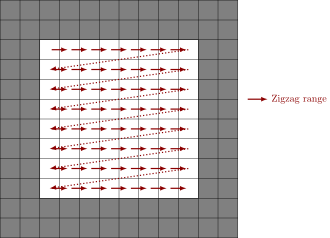
\includegraphics[width=.48\linewidth]{../figures/linear_rng}}
  \subcaptionbox{}{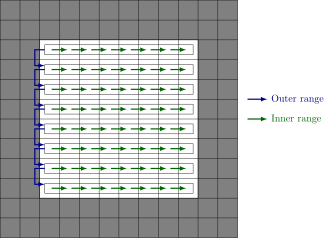
\includegraphics[width=.48\linewidth]{../figures/segmented_rng}}
  \caption{Range-v3's ranges (a) vs. multidimensional ranges (b).}
  \label{fig:inner.outer.range}
\end{figure}

Thanks to this new design we can now rewrite our algorithm with a double for-loop for the image traversing. Hopefully it
stays really similar to what one would be used to when working with the classical two-dimensional image. As an example,
we can rewrite the dilation algorithm this way:
\begin{minted}{c++}
template<class I, class SE>
auto dilate(I input, const SE& se)
{
  auto output = input.concretize(); // clone image
  // this line is needed to avoid dangling reference
  auto zipped_pixels = view::zip(input.pixels(), output.pixels());
  for(auto&& row : ranges::rows(zipped_pixels)) // unroll the contiguous segments
    for(auto [in_px, out_px] : row)             // optimized traversing of the segment
    {
      out_px.val() = out_px.val();
      for(auto nhx : se(in_px))
        out_pix.val() = std::max(in_px.val(), out_px.val());
    }
  return output;
}
\end{minted}

The highlight of this code is the usage a new tool: \texttt{ranges::rows} to bring out an inner range (contiguous) from
the multidimensional outer range.

\subsection{Performance discussion}

In order to have a relevant discussion on performance, we decided to implement a real world image processing pipeline:
the background subtraction. It is used to detect changes in image sequences~\parencite{opencv.bg_sub}. It is mainly used
when regions of interest are foreground objects. The pipeline components include: subtraction, Gaussian filtering,
threshold, erode and dilate, as shown in~\cref{fig:view.comp.sub_bg}.

\begin{figure}[htbp]
  \centering
  \includegraphics[width=0.7\linewidth]{../figures/pipeline_bg_sub_comp}
  \caption{Background subtraction pipeline using \colorbox{lightgreen}{algorithms} and
    \colorbox{thistle}{views}.}
  \label{fig:view.comp.sub_bg}
\end{figure}

The first thing that we notice is that the implementation of the pipeline using views is transcribed very explicitly in
the code, as shown in~\cref{fig:view.comp.sub_bg.view_code}. There is a direct correspondence between the graphic
pipeline and the code.

\begin{figure}
  \begin{minted}[highlightlines={3-4,6,8},highlightcolor=thistle]{c++}
  float kThreshold = 150; float kVSigma = 10;
  float kHSigma = 10;  int kOpeningRadius = 32;
  auto img_gray = view::transform(img_color, to_gray);
  auto bg_gray  = view::transform(bg_color, to_gray);
  auto bg_blurred = gaussian2d(bg_gray,  kHSigma, kVSigma);
  auto tmp_gray = img_gray - bg_blurred;
  auto thresholdf = [](auto x) { return x < kThreshold; };
  auto tmp_bin = view::transform(tmp_gray, thresholdf);
  auto ero = erosion(tmp_bin, disc(kOpeningRadius));
  dilation(ero, disc(kOpeningRadius), output);
  \end{minted}
  \caption{Pipeline implementation with \colorbox{thistle}{\emph{views}}. Highlighted code uses \emph{views} by
    prefixing operators with the namespace \texttt{view}.}
  \label{fig:view.comp.sub_bg.view_code}
\end{figure}

For our benchmark, we have decided to run the algorithm on an original set of image to detect a changing foreground.
We have considered 10 data set. We present in~\cref{fig:bg_sub.dataset_samples} three of them for the sake of brevity.

\begin{figure}[htbp]
  \centering
  \begin{tabular}{cccc}
    Background
                                                                                       & Candidate & Result                    \\[5pt]
    \fbox{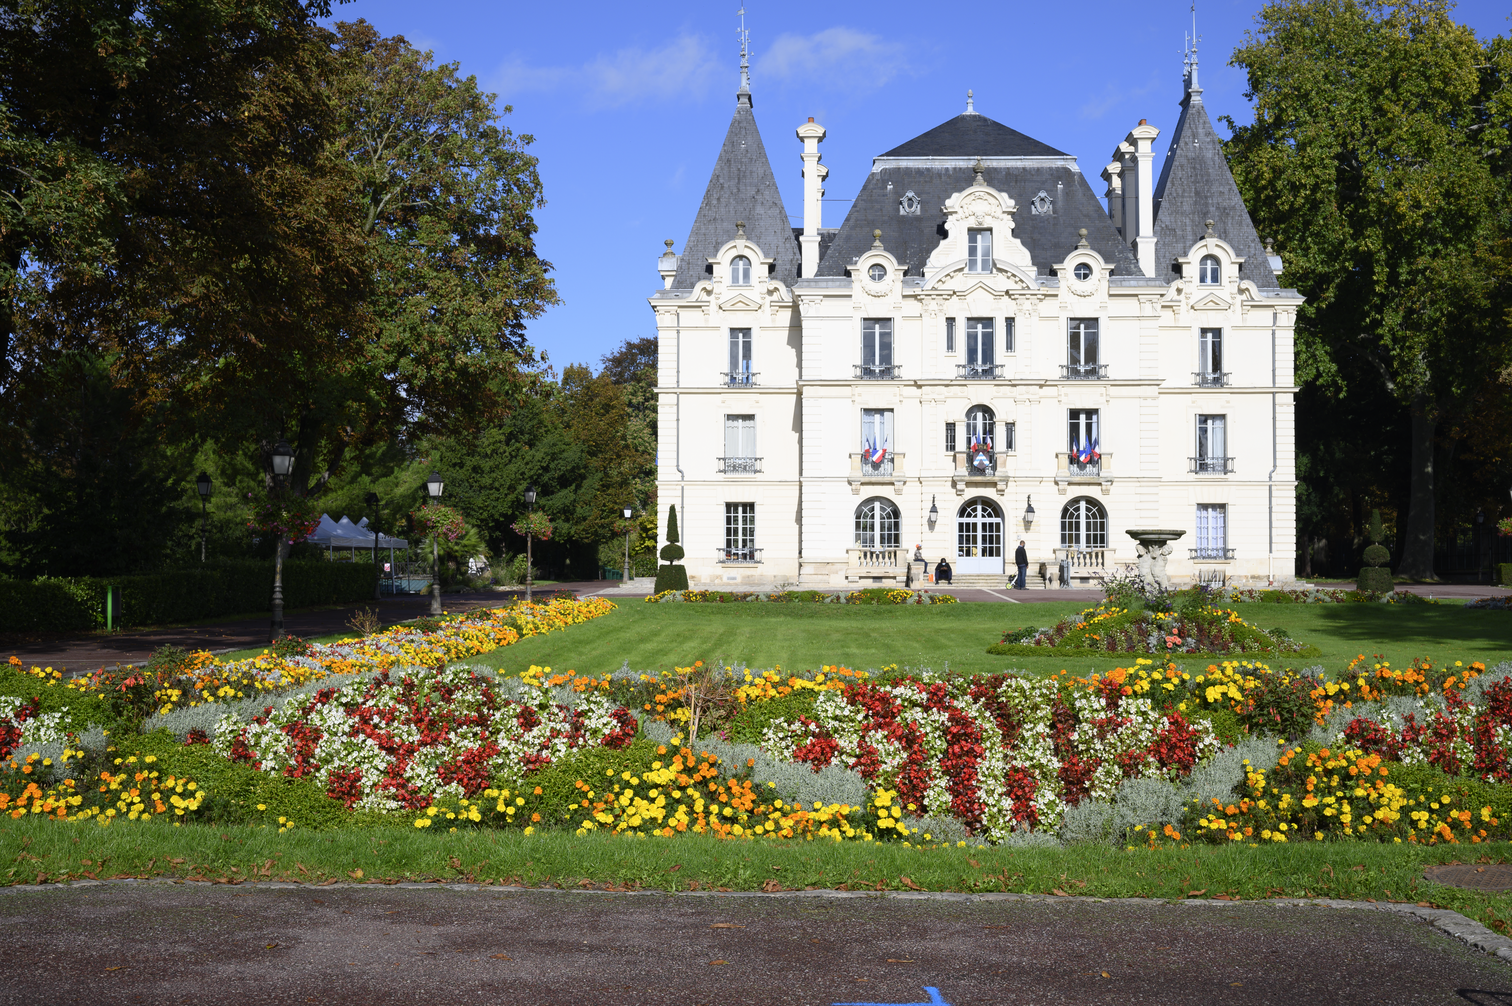
\includegraphics[width=.29\linewidth]{../assets/1512x1006/castle_bg.png}}    &
    \fbox{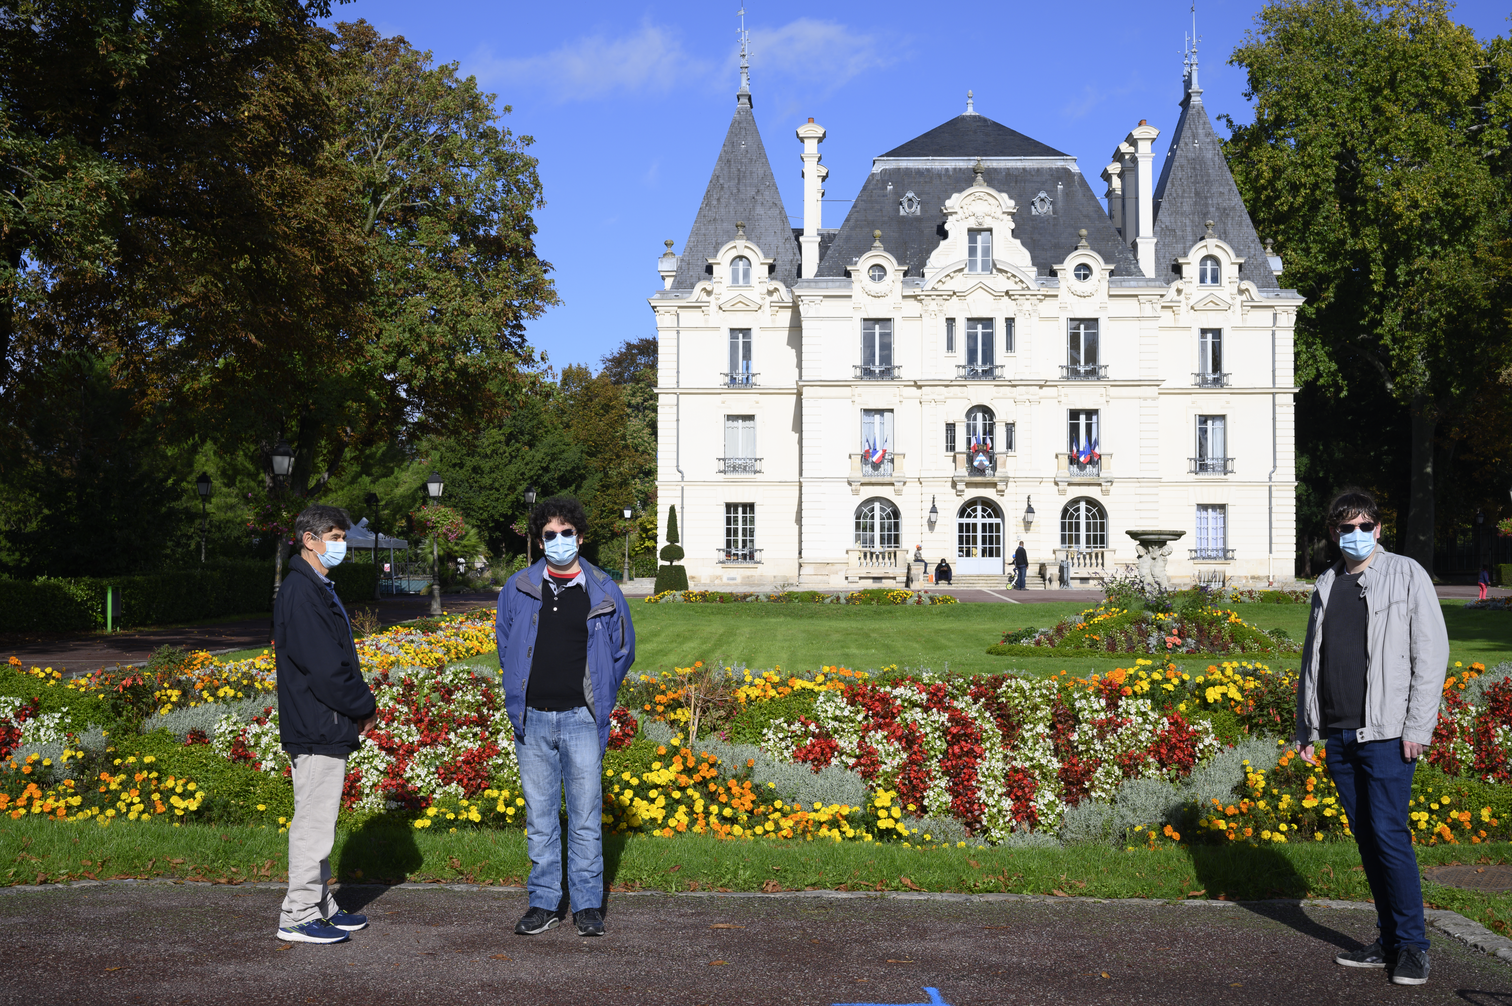
\includegraphics[width=.29\linewidth]{../assets/1512x1006/castle_fg_1.png}}  &
    \fbox{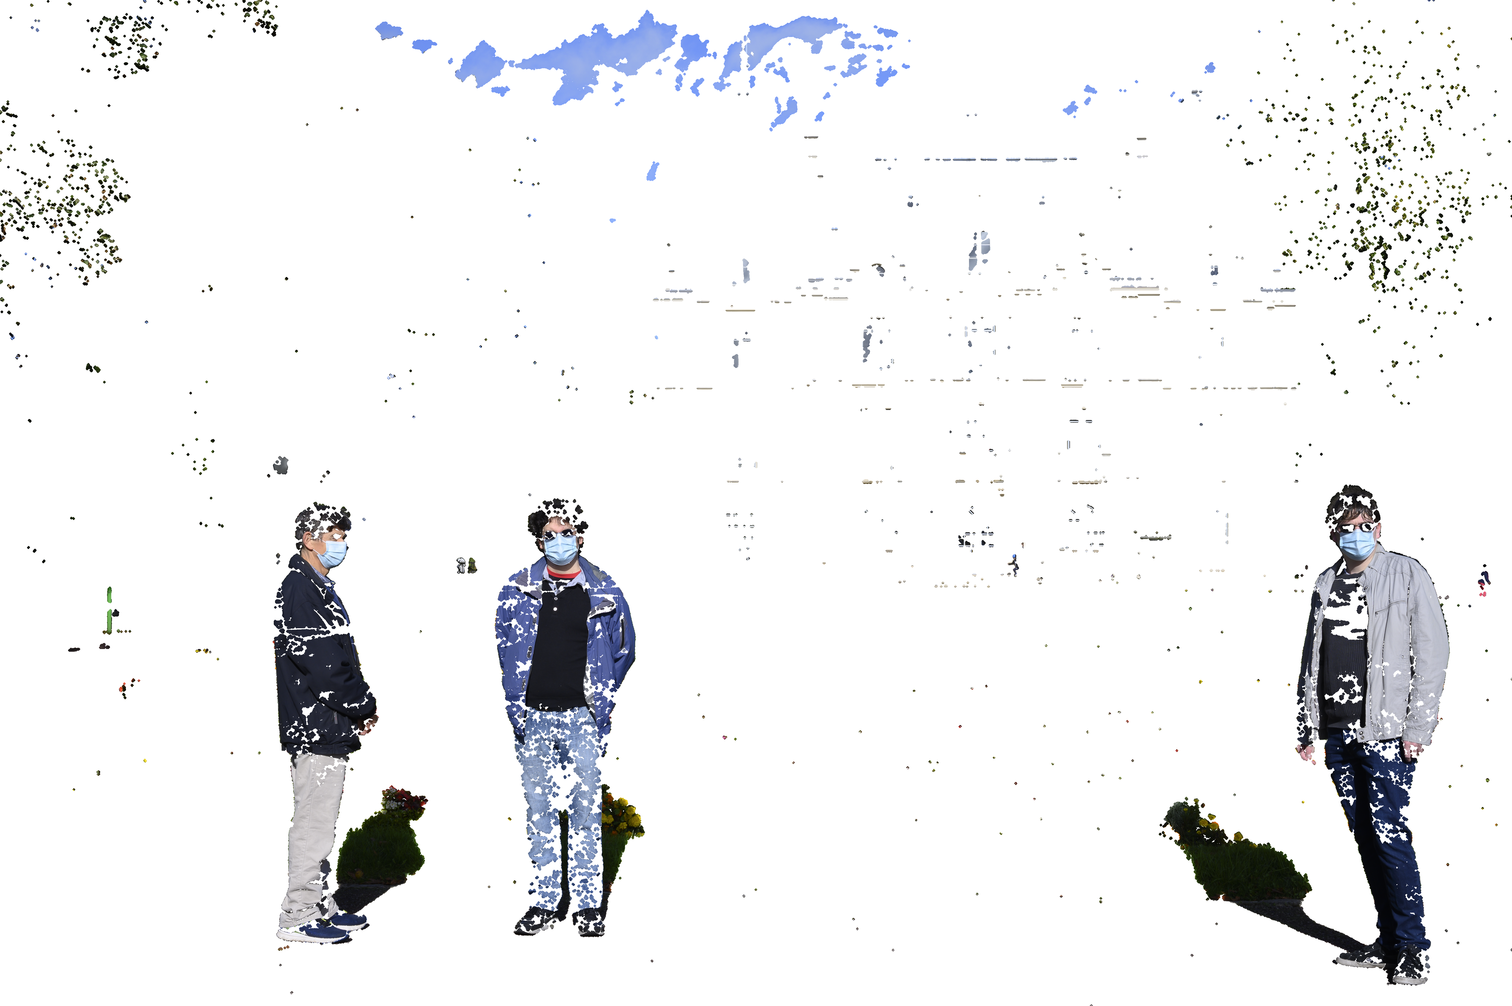
\includegraphics[width=.29\linewidth]{../assets/1512x1006/results_sig1_win5/castle/result_detected_castle_fg_1.png}} \\[5pt]
    \fbox{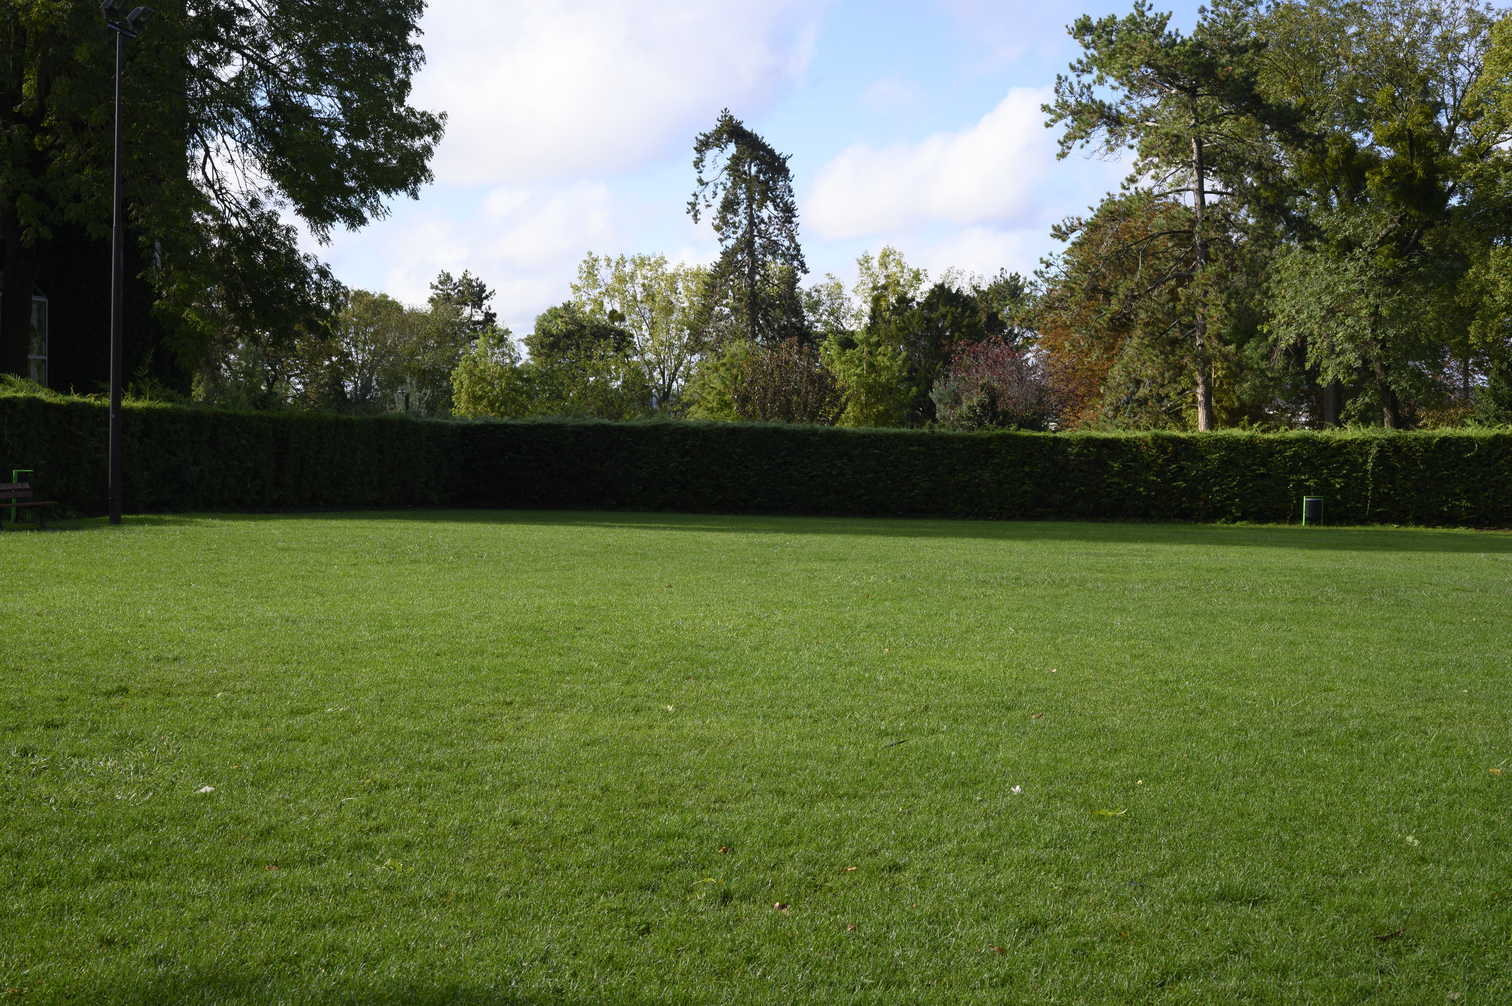
\includegraphics[width=.29\linewidth]{../assets/1512x1006/garden_bg.png}}    &
    \fbox{\includegraphics[width=.29\linewidth]{../assets/1512x1006/garden_fg_1.png}}  &
    \fbox{\includegraphics[width=.29\linewidth]{../assets/1512x1006/results_sig1_win5/garden/result_detected_garden_fg_1.png}} \\[5pt]
    \fbox{\includegraphics[width=.29\linewidth]{../assets/1512x1006/pathway_bg.png}}   &
    \fbox{\includegraphics[width=.29\linewidth]{../assets/1512x1006/pathway_fg_1.png}} &
    \fbox{\includegraphics[width=.29\linewidth]{../assets/1512x1006/results_sig1_win5/pathway/result_detected_pathway_fg_1.png}}
  \end{tabular}

  \caption{Background detection: data set samples.}
  \label{fig:bg_sub.dataset_samples}
\end{figure}

We have run benchmarks on this set comparing multiple ways of achieving this result, both using Pylene and OpenCV as
well as varying the size and the shape of the structuring element window. The breakdown of these benchmarks are
presented in~\cref{fig:bg_sub.benchmarks}. In~\cref{table:views.perf}, we benchmark the computation time and the memory
usage~\footnote{Memory usage is computed with \emph{valgring/massif} as the difference between the memory peak of the
  run and the memory peak without any computation (just setup and image loading)}of these implementations (all
single-threaded) with an opening of disc of radius 32 on 10 MPix RGB images (the minimum of many runs is kept).

\begin{figure}[htbp]
  \centering
  \begin{tabular}{cccc}
    Result                                                                                                                       & Benchmark & Benchmark Pln only \\[5pt]
    \fbox{\includegraphics[width=.29\linewidth]{../assets/1512x1006/results_sig1_win5/castle/result_detected_castle_fg_1.png}}   &
    \fbox{\includegraphics[width=.29\linewidth]{../figures/bench/PlnVsOpenCV_bg_sub_0}}                                          &
    \fbox{\includegraphics[width=.29\linewidth]{../figures/bench/PlnVsOpenCV_bg_sub_pln_0}}                                                                       \\[5pt]
    \fbox{\includegraphics[width=.29\linewidth]{../assets/1512x1006/results_sig1_win5/garden/result_detected_garden_fg_1.png}}   &
    \fbox{\includegraphics[width=.29\linewidth]{../figures/bench/PlnVsOpenCV_bg_sub_1}}                                          &
    \fbox{\includegraphics[width=.29\linewidth]{../figures/bench/PlnVsOpenCV_bg_sub_pln_1}}                                                                       \\[5pt]
    \fbox{\includegraphics[width=.29\linewidth]{../assets/1512x1006/results_sig1_win5/pathway/result_detected_pathway_fg_1.png}} &
    \fbox{\includegraphics[width=.29\linewidth]{../figures/bench/PlnVsOpenCV_bg_sub_6}}                                          &
    \fbox{\includegraphics[width=.29\linewidth]{../figures/bench/PlnVsOpenCV_bg_sub_pln_6}}
  \end{tabular}

  \caption{Background detection: garden results.}
  \label{fig:bg_sub.benchmarks}
\end{figure}

\newcommand{\mystd}[1]{{\itshape(\(\pm\) #1)}}
\newcommand{\mydelta}[1]{{\itshape\bfseries #1\%}}

\begin{table}
  \centering
  \begin{tabular}{l|ccc}
    \toprule
    Framework          & Compute Time            & Memory usage & \(\Delta{}\)Memory usage \\ \midrule
    Pylene (w/o views) & \(2.11s\) \mystd{144ms} & 106 MB       & \mydelta{+0}             \\
    OpenCV             & \(2.41s\) \mystd{134ms} & 59 MB        & \mydelta{-44}            \\
    Pylene (views)     & \(2.13s\) \mystd{164ms} & 51 MB        & \mydelta{-52}            \\
    \bottomrule
  \end{tabular}
  \caption{Benchmarks of the pipeline \cref{fig:view.comp.sub_bg} on a dataset (12 images) of 10MPix images. Average
    computation time and memory usage of implementations with/without \emph{views} and with OpenCV as a baseline.}
  \label{table:views.perf}
  %\vspace{-1em}
\end{table}

The results should not be misunderstood. They do not say that OpenCV is faster or slower but shows that implementations
all have the same order of processing time (the algorithms used in our implementation are not the same as those used in
OpenCV for blur and dilation/erosion) so that the comparison makes sense. It allows us to validate experimentally the
advantages of views in pipelines. First, we have to be cautious about the real benefit in terms of processing time.
Here, most of the time is spent in algorithms that are not eligible for view transformation. Thus, depending on the
operations of the pipeline, views may not improve processing time. Nevertheless, using views does not degrade
performance neither (only 1\% in this experiment). It seems to show that using views does not introduce performance
penalties and may even be beneficial in lightweight pipelines as the one in~\cref{fig:view.pipeline}. On the memory
side, views reduce drastically the memory usage (also seen in~\cref{fig:legacy.vs.view}) which is beneficial when
developing applications which are memory constrained. From the developer standpoint, it requires only few changes in the
code as shown in~\cref{fig:view.comp.sub_bg.view_code} — the implementation of the algorithms remain the same — which is
a real advantage for software maintenance.


\section{Summary}

\paragraph{Views are composable.} One of the most important feature in a pipeline design (generally, in software
engineering) is \emph{object composition}. It enables composing simple blocks into complex ones. Those complex blocks
can then be managed as if they were still simple blocks. In~\cref{fig:view.pipeline}, we have 3 simple image processing
operators \emph{Image}~\(\rightarrow\)~\emph{Image} (the grayscale conversion, the sub-quantization and the dilation).
As shown in~\cref{fig:view.comp}, algorithm composition would consider these 3 simple operators as a single complex
operator \emph{Image}~\(\rightarrow\)~\emph{Image} that could then be used in another even more complex processing
pipeline. Just like algorithms, image views are composable, e.g. a view of the view of an image is still an image.
In~\cref{fig:view.comp}, we compose the input image with a grayscale transform view and a sub-quantization view that
then feeds the dilation algorithm.

\paragraph{Views improve usability.} The code to compose images in~\cref{fig:view.comp} is almost as simple as:

\begin{minted}{c++}
auto input = imread(...);
auto A = transform(input, [](rgb16 x) -> float {
  return (x.r + x.g + x.b) / 3.f; }; );
auto MyComplexImage = transform(A, [](float x)
  -> uint8_t { return (x / 256 + .5f); }; );
\end{minted}

People familiar with functional programming may notice similarities with these languages where \emph{transform}
(\emph{map}) and \emph{filter} are sequence operators. Views use the functional paradigm and are created by functions
that take a function as argument: the operator or the predicate to apply for each pixel; we do not iterate by hand on
the image pixels.

\paragraph{Views improve re-usability.} The code snippets above are simple but not very re-usable. However, following
the functional programming paradigm, it is quite easy to define new views, because some image adaptors can be considered
as \emph{high-order functions} for which we can bind some parameters, as one would do with the curry
technique~\parencite{hanus.1995.curry}. In~\cref{fig:view.highorder}, we show how the primitive \emph{transform} can be
used to create a view summing two images and a view operator performing the grayscale conversion as well as the
sub-quantization which can be reused afterwards\footnote{These functions could have been written in a more generic way
  for more re-usability, but this is not the purpose here.}.

\begin{figure}
  \begin{minted}{c++}
auto operator+(Image A, Image B) {
  return transform(A, B, std::plus<>());
}
auto togray = [](Image A) { return transform(A, [](auto x)
  { return (x.r + x.g + x.b) / 3.f; };)
};
auto subquantize16to8b = [](Image A) { return transform(A,
  [](float x) { return uint8_t(x / 256 +.5f); });
};

auto input = imread(...);
auto MyComplexImage = subquantize16to8b(togray(A));
  \end{minted}

  \caption{Using high-order primitive views to create custom view operators.}
  \label{fig:view.highorder}
\end{figure}

\paragraph{Views for lazy computing.} Because the operation is recorded within the image view, this new image type
allows fundamental image types to be mixed with algorithms. In~\cref{fig:view.highorder}, the creation of views does not
involve any computation in itself but rather delays the computation until the expression \texttt{v(p)} is invoked.
Because views can be composed, the evaluation can be delayed quite far. Image adaptors are \emph{template
  expressions}~\parencite{veldhuizen.1995.expression,veldhuizen.2000.blitz} as they record the \emph{expression} used to
generate the image as a template parameter. A view actually represents an expression tree (\cref{fig:new.alphablend}).

\paragraph{Views for performance.} With a classical design, each operation of the pipeline is implemented on ``its
own''. Each operation requires memory to be allocated for the output image and also, each operation requires that the
image is fully traversed. This design is simple, flexible, composable, but is not memory efficient nor computation
efficient. With the lazy evaluation approach, the image is traversed only once (when the dilation is applied) which has
two benefits. First, there are no intermediate images which is very memory efficient. Second, traversing the image is
faster thanks to a better memory cache usage, and performs an optimal selective traversal. Indeed, in our example
(\cref{summary:fig:view.pipeline}), processing a RGB16 pixel from the dilation algorithm directly converts it in
grayscale, then sub-quantize it to 8-bits, and finally makes it available for the dilation algorithm. It acts \emph{as
  if} we were writing an optimal operator that would combine all these operations. This approach is somewhat related to
the kernel-fusing operations available in some HPC specifications~\parencite{openvx.2019} but views-fusion is optimized
by the C++ compiler only~\parencite{brown.2018.ranges}. The selective aspect intervenes when a region of interest is
selected at one point in the processing pipeline. Indeed, the entirety of the pipeline is then executed only on the
region of interest, even if this selection happens only at the very end of the processing pipeline.

\paragraph{Views for productivity.} All point-wise image processing algorithms can (and should) be rewritten intuitively
by using a one-liner view. The \emph{transform} views is the key enabling that point. This implies that there exist a
new abstraction level available to the practitioner when prototyping their algorithm. The time spent implementing
features is reduced, thus the feedback-loop time is reduced too. This naturally brings productivity gain to the
practitioner.


\cleardoublepage

\chapter{Static dynamic bridge}
\label{chap.static_dynamic_bridge}

%\section{Coexistence between the static world and the dynamic world}
%introduction

In the programming world, there are two main families of programming language. There are the \emph{compiled}
programming, such as C, C++, Rust or Go. There are also the \emph{interpreted} programming languages, such as Python,
PHP, Lisp or Javascript. Finally, there are languages such as Java that are both at the same time.

The \emph{compiled} programming languages have the advantage of being very end-user friendly. Indeed, the implementer
distribute compiled self-sufficient binaries and the user select the binary that is compatible with his operating
system. Then, the program is supposed to work out of the box without more work than that, as illustrated
in~\cref{fig:static.dynamic.compiled.runtime}.

\begin{figure}[tbh]
  \centering
  \includegraphics[width=.6\linewidth]{figs/static_runtime}
  \caption{Compiled languages: run-time}
  \label{fig:static.dynamic.compiled.runtime}
\end{figure}

Opposite to this apparent simplicity for the end-user, all the burden is shouldered by the programmer. Indeed, to
generate a binary, there are many steps, as illustrated in~\cref{fig:static.dynamic.compiled.compiletime}. There is a
first pass with the compiler to generate intermediate machine code. Then there is a linker pass to resolve any
dependency between machine code and system code into one or multiple final distributable binaries. However, this last
pass tie the binary with a distribution. Indeed, the location of system libraries may vary between operating system,
between version of the same operating system, between compiler variants etc. Also, as the developer wants to distribute
efficient programs, he will use last optimized vectorized instructions if possible, which can tie further the binary to
a certain set of hardware supporting some assembly instructions (SSE4, XOP, FMA4, AVX-512, etc.). Upstream from those
issues, there are also issues with code. Indeed, many libraries are not cross-platform and leveraging all the
equivalences from one OS to another incurs an increase in code quantity, tests and maintenance cost to support many
platforms. For instance, the native GUI Windows libraries does not exist in Linux and must be rewritten with another
framework, such as GTK or Qt. Or else, the developer can choose to use a cross-platform GUI library from start however
this decision may not have been viable if the software was first windows-only and the cross-platform support was added
at a later date. Another caveat is that using code introspection is often very difficult at compile-time because only
few information are available (only static information). Dynamic reflection at runtime is impossible.

\begin{figure}[tbh]
  \centering
  \includegraphics[width=.6\linewidth]{figs/static_compiletime}
  \caption{Compiled languages: compile-time}
  \label{fig:static.dynamic.compiled.compiletime}
\end{figure}

The \emph{interpreted} programming language are a little less end-user friendly but are much more comfortable for
developer to distribute their software. Indeed, as shown in~\cref{fig:static.dynamic.dynamic.pipeline}, everything
happens at runtime. The maintainer only distribute the source code, the dependency list and the assets necessaries for
his program. The burden is mostly shouldered by the end-user this time. He must download and install all the language
interpreter and environment in order to execute the program from the source code. He must resolve the dependencies and
be able to execute the source code on his computer. This has the advantage of having a very rich ecosystem as
distributing, maintaining and using programs is very easy once integrated in a package manager (often delivered with the
language SDK natively). However, the main disadvantage is the performance. As the source code is not compiled into
optimized assembly code ready to be executed, the interpreter must do all the work in one go and very often this is
slow. Nowadays, all the interpreter embarks a Just-In-Time (JIT) compiler that detected the portions of a program that
are used heavily (a.k.a. hot code) and will compile them into native machine code to increase the performance
drastically without having the user pay for a long compilation time. Also, those languages usually have very developed
introspection facilities. Dynamic reflection at runtime is possible and some language, such as Common Lisp, even go
further by allowing the developer to mutate the program Abstract Syntax Tree (AST) at runtime (macro). This allows very
powerful integrations such as defining one's own DSL as if it was part of the core language itself.

\begin{figure}[tbh]
  \centering
  \includegraphics[width=.6\linewidth]{figs/dynamic_pipeline}
  \caption{Compiled languages: compile-time}
  \label{fig:static.dynamic.dynamic.pipeline}
\end{figure}

Image processing communities like to have bridges with interpretable language such as Python or Matlab, to interface
with their favorite tools, algorithms and/or facilities. As an example, with Python, the module
NumPy~\cite{oliphant.2006.numpy} is community standard which is heavily used. Henceforth, to broaden the usage of our
library, we should be able to provide a way to communicate between our library and NumPy. However here is a showstopper:
we only distribute source code, we don't hand over binaries. Indeed, genericity in C++ is achieved via usage of template
metaprogramming. One caveat of it is that the C++ compiler cannot generate a binary until it knows which type (of image,
of value) will be used. But we don't know this information: the user (on Python's end) is not going to recompile our
library each time he has another set of types to exercise. From here, there are still multiple ways to achieve our goal.

First option is to embark a JIT (Just-in-time) compiler whose job would be to generate the binaries and bindings just as
they are used. This solution brings speed (excluding the first run that includes the compilation time) and unrestrained
genericity. However we are now bound to specificities of a compiler vendor and loose platform portability.

Another option is to type-erase our types to enables the use of various concrete types through a single generic
interface. This would translate into a class hierarchy whose concrete classes are on the leaves (thus, whose value type
and dimension are known). This induces a non negligible slow down but allow us to keep the genericity and portability at
the cost of maintaining the class hierarchy.

Type generalization can also be considered: cast everything into a super-type that is suitable for the vast majority of
cases. For instance, we could say that we have a super-type \texttt{image4D<double>} into which we can easily cast
sub-types such as \texttt{image2D<int>} or \texttt{image3D<float>}. Of course we would loose the generic aspect and
induce non negligible speed cost. Although portability is kept.

And finally there is the dynamic dispatch. It consists in embarking dynamic information at runtime about types, and
dispatch (think of switch/case) to the correct facility which can handle those types. The obvious caveat is the cost of
maintenance induced by the genericity as we would have a number of possible dispatches that grow in a multiplicative way
with the number of handled types. Which is not very generic. On the other hand there is almost no speed loss and the
portability is guaranteed. Theoretical models exists that could bring solutions to lower the number of dispatcher to
write, such as multi-method~\cite{pirkelbauer.2010.multimethods}. Unfortunately they are currently not part of C++.

%\section{Design hybrid solution, motivations and choices}

%\FIXME{TODO: schémas solution hybride, arbre de dispatching etc.}

\section{Hybrid solution: type-erasure and $n*n$ dispatch}


In Pylene we have chosen an hybrid solution between type-erasure and dynamic dispatch. The aim is to have a set of known
types for which we have no speed cost as well as continuing to handle other types to remain generic. To achieve this
goal, we have worked together with Célian Gossec~\cite{gossec.2019.pybind}, a student co-supervised by the authors of
this thesis, in order to provide a facility to expose our generic code to Python. As seen in the previous chapter, it is
not possible to bind C++ source code to Python. We need to have a compiled binary implementing Python binding (we chose
Pybind11~\parencite{jakob.2017.pybind11}) in order to be able to call C++ code from Python. In order to achieve the
binding without sacrificing the genericity and the performances, we have designed a solution in two steps. We do not
want to provide an abstract interface that will resolve the calls to access data on the call-site via virtual call
because it would be very slow when the C++ code is executed. This would defeat the purpose of having to rely on C++ in a
first place. However, it is possible to convert an abstract class into an instantiated concrete generic class whose
template parameter are known. This requires, however, to enumerate all the possible cases. With modern C++, it has
become possible to design $n*n$ dispatch without gigantic switch-case clauses.

\subsection{First step: type-erasure}

The first step of our solution consists in designing a buffer class that holds all the informations about an image:
dimension, underlying type, strides and pointer to data buffer. This class is named \texttt{ndimage\_buffer}. When
interfacing with Python, it is necessary to convert the Python image which is a \texttt{NumpPy.array} into our image
type. The purpose of this buffer image is to holds all the informations from the \texttt{NumpPy.array} to then
instantiate a concrete C++ type. The first pitfall here is due to a limitation from the abstraction interface used in
Python. Indeed, when using for instance \emph{Scikit-Image}, it is not possible to differentiate a 2D multichannel image
from a 3D grayscale image. Indeed, the image is always broken down to its most simple value and a 3D multichannel image
is turned into a 3-dimensional \texttt{NumpPy.array} containing 8-bits values, the last dimension contains only 3
elements at max but can theoretically contain more as there is no limitation from the used abstraction to prevent that.
A 3D grayscale image will be broken down into a 3-dimensional \texttt{NumpPy.array} containing 8-bits values, the last
dimension will contain many values as it is expected of a 3D-image. To prevent this confusion, there is a need to
explicitly say to the Python/C++ wrapper wether the image is multichannel or not. This information must be carried
through the \texttt{ndimage\_buffer} into C++ for a correct instanciation. This process is illustrated
in~\cref{fig:type-erased.buffer}.

\begin{figure}[tbh]
  \centering
  \includegraphics[width=.6\linewidth]{figs/type-erased_buffer}
  \caption{Bridge from Python to C++ via Pybind11 and a type-erased C++ class.}
  \label{fig:type-erased.buffer}
\end{figure}

From the point of view of a practitioner, the code on the call-site (python side) should be as follow:
\begin{minted}{python}
  from skimage import data
  import numpy as np
  import Pylena as pln # our python binding
  img = data.astronaut() # 2D-rgb8 image -> Numpy.array(ndim=3, dtype='uint8')
  pln_img = pln.ndimage(img, multichannel=True) # manualy point out multichannel information
  # use(pln_img) for any pln.<algorithm> exposed to Python
\end{minted}

From the point of view of the library implementer, the code to expose the binding looks like this one:
\begin{minted}{C++}
  #include "ndimage.hpp"
  #include <pybind11/pybind11.h>

  // Expose pybind module
  void init_class_ndimage(pybind11::module& m);
  PYBIND11_MODULE(Pylena, m) { init_class_ndimage(m); }

  // declare the conversion function
  namespace mln::py {
    mln::ndbuffer_image   ndimage_from_buffer(pybind11::buffer b);
    pybind11::buffer_info ndimage_to_buffer(const mln::ndbuffer_image& img);
  }

  // expose the python ndimage class with the conversion from/to py::buffer (numpy.array buffer)
  void init_class_ndimage(py::module& m)
  {
    py::class_<mln::ndbuffer_image>(m, "ndimage", py::buffer_protocol())
        .def(py::init([](py::buffer b, bool multichannel) {
          return mln::py::ndimage_from_buffer(b, multichannel); }))
        .def_buffer(mln::py::ndimage_to_buffer);
  }
\end{minted}

This code declares a new module named \texttt{Pylena}. It then declares a class named \texttt{ndimage} which is a bridge
to Python's \texttt{buffer\_protocol}. This \texttt{buffer\_protocol} is an abstraction to allow the usage of NumPy's
array. Finally, the code declares that the class is convertible to and from the \texttt{buffer\_protocol} thanks to
provided callbacks. The code of those callbacks is as follow:

\begin{minted}{C++}
  // implement the conversion from Python to C++
  mln::ndbuffer_image ndimage_from_buffer(::py::buffer b, bool is_multichannel)
  {
    /* Request a buffer descriptor from Python */
    ::py::buffer_info info = b.request();

    std::ptrdiff_t      strides[16];
    int                 dims[16];
    int                 ndim = info.ndim - is_multichannel ? 1 : 0;
    int                 bpp  = info.itemsize;

    // convert the type information from Python to C++ (string to enum) for faster dispatch
    mln::sample_type_id st   = get_sample_type(info.format, is_multichannel);

    for (int i = 0; i < ndim; ++i) {
      dims[i]    = info.shape[ndim - 1 - i];
      strides[i] = info.strides[ndim - 1 - i];
    }

    if (strides[0] != bpp)
      throw std::runtime_error("Unsupported image stride along the last dimension.");

    // construct the type-erased image with all informations
    return mln::ndbuffer_image::from_buffer(
      reinterpret_cast<std::byte*>(info.ptr), st, ndim, dims, strides);
  }

  // implement the conversion from C++ to Python
  ::py::buffer_info ndimage_to_buffer(const mln::ndbuffer_image& img)
  {
    // return the python format of the underlying type, as well as information about multichanneling
    auto [ti, is_multichannel] = get_sample_type_id_traits(img.sample_type());

    int ndim = img.pdim() + is_multichannel ? 1 : 0;

    std::vector<ssize_t> dims(ndim);
    std::vector<ssize_t> strides(ndim);

    for (int i = 0; i < ndim; ++i) {
      dims[i]    = img.size(ndim - 1 - i);
      strides[i] = img.byte_stride(ndim - 1 - i);
    }
    // construct the python buffer with all the information
    return ::py::buffer_info(img.buffer(), ti.size(),
            get_sample_type(img.sample_type(), multichannel), ndim, dims, strides);
  }
\end{minted}

This code forward informations about the buffer and handle the special case of multichannel images which Python treat
as 3D images.

\subsection{Second step: multi-dispatcher}
The second step of our hybrid solution is to dispatch the type-erased code to efficient generic code. The naive way of
doing so would be to include a gigantic switch-case clause in each algorithm implementation and dispatch to the correct
instantiated generic algorithm from there. Aside from being a nightmare to maintain, the size of those clause can grow
several fold depending on the cardinality of the generic implementation. For instance, for a generic dilation, there are
3 axis of cardinality: the underlying type, the dimension, the structuring element shape. In the case where the library
support 5 different structuring element shape, 10 underlying types and 6 dimension for the image, the switch-case
statement will have 300 clauses to dispatch. And each algorithm will have to dispatch. This solution is not viable,
defeat the purpose of genericity which is to write less code in the first place. We had to find a solution to have those
dispatch while keeping our code short and efficient. The idea we took to solve this problem comes from the design of a
C++ feature, the variant, and especially the visitor. We need to have a way to write the implementation of the algorithm
once while enumerating all the possible cases. Also, if possible, the list of supported types should be written once at
one place for maintenance purpose.

We then had the idea of writing a dispatcher. This dispatcher list all the supported types and call the given callbacks
forwarding the given arguments by instantiating a specific type. For instance, let us first expose the binary threshold
operator to Python. The Python call-site code will look like this:

\begin{minted}{python}
  img_grayscale = skimage.data.grass()
  pln.operators.binary_threshold(img_grayscale)
\end{minted}

On C++ side, we need to expose the function with this code:
\begin{minted}{C++}
  void init_module_operators(pybind11::module& m);

  mln::ndbuffer_image binary_threshold(::py::buffer buffer)

  void init_module_operators(::py::module& m) {
    using namespace pybind11::literals;

    m.def("binary_threshold", binary_threshold,
          "Perform a binary threshold.\n",
          "Input"_a);
  }

  PYBIND11_MODULE(Pylena, m) {
    /* ... */

    auto operators = m.def_submodule("operators", "Image processing operators.");
    init_module_operators(operators);
  }
\end{minted}

Now that our python submodule and that our \texttt{binary\_threshold} operator are declared, let us have a look to the
operator's implementation:

\begin{minted}{C++}
  mln::ndbuffer_image dilate(::py::buffer buffer)
  {
    // grayscale image mandatory
    auto input = mln::py::ndimage_from_buffer(buffer);

    // dispatch along dimension (dimension is a valued template parameter, hence _v)
    return dispatch_v<binary_threshold_operator_t>(input.pdim(), input);
  }
\end{minted}

We have replaced the gigantic switch-case clause by a dispatcher templated by an operator. This operator will cast the
input image into the concrete generic type and call the fast generic algorithm on it. Let us have a look to what this
operator look like:

\begin{minted}{C++}
  // Operator templated by the dimension
  template <auto Dim>
  struct binary_threshold_operator_t {
    // Function templated by the image type
    template <typename Img>
    mln::ndbuffer_image operator()(Img&& img) const {
      // Cast to a grayscale (information known) of the correct dimension
      if (auto* image_ptr = std::forward<Img>(img).template cast_to<std::uint8_t, Dim>(); image_ptr)
        // call generic algorithm
        return mln::operators::binary_threshold(*image_ptr);
      else {
        std::runtime_error("Unable to convert the image to the required type.");
        return {};
      }
    }
  };
\end{minted}

This operator will attempt to cast the given image into a grayscale image of the correct dimension and then use the
resulting concrete type to pass it the fast generic \texttt{binary\_threshold} operator. Now let us have a look at where
the magic happen, at the dispatcher which list all the supported type.

\begin{minted}{C++}
template <template <auto> class V, typename... Args>
auto dispatch_v(std::size_t dim, Args&&... args) {
  switch (pdim) {
  case (1):
    return F<1>{}(std::forward<Args>(args)...);
  case (2):
    return F<2>{}(std::forward<Args>(args)...);
  case (3):
    return F<3>{}(std::forward<Args>(args)...);
  case (4):
    return F<4>{}(std::forward<Args>(args)...);
  case (5):
    return F<5>{}(std::forward<Args>(args)...);

  /* ... */

  case (0):
    [[fallthrough]];
  default:
    throw std::runtime_error("Unsupported dimension.");
}
\end{minted}

The dispatcher is instantiate the given type by the correct dimension number and then call the operator parenthesis
(function call) forwarding all the given parameters. In our case, it will instantiate the type
\texttt{binary\_threshold\_operator\_t<2>} and then call the function
\texttt{binary\_threshold\_operator\_t<2>.operator()(input)}, forwarding the input image to the underlying algorithm.

The main advantage of this approach is that all the supported features are to be listed only in one place, the
dispatcher, while any number of dispatcher can be piped to achieve the cardinality wanted. Let us push our example to
implement the mathematical morphology operator dilation. We now have two more generic axis to cover: the structuring
element shape and the underlying datatype. First, let us expose the operator to the Python code. Here is what the Python call-site look like:

\begin{minted}{python}
img_grayscale = skimage.data.grass()
rect = pln.se.rect2d(width=3, height=3)
pln.operators.dilate(img_grayscale, se)
\end{minted}

We need to expose the new structuring element's sub-module for usage in the dilation operator:

\begin{minted}{C++}
void init_module_se(pybind11::module& m);

void init_module_se(::py::module& m) {
  ::py::class_<mln::se::disc>(m, "disc").def(
      ::py::init([](float radius) { return mln::se::disc{radius}; }));

  ::py::class_<mln::se::sphere>(m, "sphere").def(::py::init([](float radius) {
    return mln::se::sphere{radius};
  }));

  ::py::class_<mln::se::rect2d>(m, "rect2d").def(::py::init([](int width, int height) {
    return mln::se::rect2d{width, height};
  }));

  ::py::class_<mln::se::rect3d>(m, "rect3d").def(::py::init([](int width, int height, int depth) {
    return mln::se::rect3d{width, height, depth};
  }));
}

PYBIND11_MODULE(Pylena, m) {
  /* ... */

  auto mse = m.def_submodule("se", "Structuring elements module.");
  init_module_se(mse);
}
\end{minted}

Now we need to expose the dilate function into the operator submodule:
\begin{minted}{C++}
// using std::variant
using se_t = std::variant<mln::se::disc, mln::se::sphere,
                          mln::se::rect2d, mln::se::cube>;

mln::ndbuffer_image dilate(::py::buffer buffer, const se_t& se)

void init_module_operators(::py::module& m) {
  /* ... */

  m.def("dilate", dilate,
    "Perform a morphological dilation.\n"
    "\n"
    "structuring element must be valid.",
    "Input"_a, "se"_a);
}
\end{minted}

We are all set to now implement the dilation operator. First, let us have a look at the underlying operator that will be
dispatched:

\begin{minted}{C++}
template <auto Dim, typename T>
struct dilate_operator_t {
  template <typename Img, typename SE>
  mln::ndbuffer_image operator()(Img&& img, SE se) const {
    if (auto* image_ptr = std::forward<Img>(img).template cast_to<T, Dim>(); image_ptr)
      return mln::dilation(*image_ptr, se);
    else {
      std::runtime_error("Unable to convert the image to the required type.");
      return {};
    }
  }
};
\end{minted}

Here we can see that we need a double dispatch. Also, the structuring element is no longue a variant and needs to be
dispatched before instantiating this operator. Finally, there is an issue here because there are two template parameter
and our dispatcher \texttt{dispatch\_v} does only handle one. We workaround this issue by writing another intermediate
operator dispatcher \texttt{dilate\_operator\_intermediate\_t} serving as trampoline that will partially instantiate the
final operator \texttt{dilate\_operator\_t} along the dimension template parameter to feed it to the last dispatcher,
\texttt{dispatch\_t}:

\begin{minted}{C++}
template <auto Dim>
struct dilate_operator_intermediate_t {
  template <typename Img, typename SE>
  mln::ndbuffer_image operator()(Img&& img, SE&& se) const {
    // Partial instantiation
    return double_dispatch_t<dilate_operator_t, Dim>(
            input.sample_type(), std::forward<Img>(input), std::forward<SE>(se));
  }
};
\end{minted}

The final function implementation will look like this:

\begin{minted}{C++}
mln::ndbuffer_image dilate(::py::buffer buffer, const se_t& se) {
  auto input = mln::py::ndimage_from_buffer(buffer);
  // dispatch the structuring elements through using std::visit for std::variant 
  return std::visit(
      [&input](const auto& se_) {
        return dispatch_v<dilate_operator_intermediate_t>(input.pdim(), input, se_);
      }, se);
}
\end{minted}

The final piece of our puzzle would be the double dispatch function that will handle the last dispatch along the
underlying data while forwarding the first dispatch along the dimension. Here is how we implemented our double dispatch:

\begin{minted}{C++}
template <template <auto, typename> class F, auto Dim, typename... Args>
auto double_dispatch_t(mln::sample_type_id tid, Args&&... args) {
  switch (tid) {
    case (mln::sample_type_id::INT8):
      return F<Dim, std::int8_t>{}(std::forward<Args>(args)...);
    case (mln::sample_type_id::INT16):
      return F<Dim, std::int16_t>{}(std::forward<Args>(args)...);
    case (mln::sample_type_id::INT32):
      return F<Dim, std::int32_t>{}(std::forward<Args>(args)...);
    case (mln::sample_type_id::UINT8):
      return F<Dim, std::uint8_t>{}(std::forward<Args>(args)...);
    case (mln::sample_type_id::UINT16):
      return F<Dim, std::uint16_t>{}(std::forward<Args>(args)...);
    case (sample_type_id::UINT32):
      return F<Dim, std::uint32_t>{}(std::forward<Args>(args)...);
    case (mln::sample_type_id::DOUBLE):
      return F<Dim, double>{}(std::forward<Args>(args)...);

      /* ... */

    case (mln::sample_type_id::OTHER):
      [[fallthrough]];
    default:
      throw std::runtime_error("Unhandled data type");
  }
}
\end{minted}

Now we have all the pieces to build operators that are agnostic from the supported data-types. Indeed, the maintainer
has gathered all the logic about listing supported data types and dimension into variant or custom dispatcher. He just
need to maintain those to enable, by default, all exposed algorithm to support them. This hybrid solution mixes
type-erasure and modern C++ facilities to allow maximum performance. Indeed, the dispatch is done before entering
algorithms and the buffer protocol facility allows us to plug directly into the Python image without having any
unnecessary copies. The only caveat would be the code bloat incurred by all the explicit instanciation leading to
compiling a large binary. Another point not covered right now would be a way to inject Python types into C++. Indeed,
our hybrid solution only support the types provided by the library. It will instantiate all the code relative to them
and support all of the combinations. But the user may be tempted to plug a user-defined type from Python as an
underlying data-type. To allow this use-case, we introduce a new concept: the value-set. The value-set is a standard way
manipulate the underlying values. Through type-erasure, we can either manipulate a known underlying value with native
facilities (near-zero overhead) or fallback on a virtual call that may report an error or callback user-provided Python
routine to manipulate an unknown user value.

\subsection{Third and final step: the value-set}

\FIXME{TODO: write subsection.}

\subsection*{Material for value-set}


Let us illustrate this path with an example: the stretch algorithm. First let's see the naive algorithm:
\begin{minted}{C++}
  template <typename T>
  image2d<float> stretch(const image2d<T>& src)
  {
    auto res = image2d<float>(src.width(), src.height());
    auto values_span = src.values();
    std::transform(values_span.begin(), values_span.end(), res.values().begin(),
      [](T val) -> float
      {
        return static_cast<float>(val) / std::numeric_limits<T>::max();
      }
    );
    return res;
  }
\end{minted}

One should observe that the function parameter is templated by a type \texttt{T}. This induces that "span" further in
the code is also templated. Both needs to be type erased. Furthermore, getting the max value of the type \texttt{T} is
also an issue that needs to be abstracted away.

We aim at obtaining this prototype:

\begin{minted}{C++}
  image2d<> stretch_py(const image2d<>& src);
\end{minted}

Here \texttt{image2d<>} which is also \texttt{image2d<void>} is the type-erased type of \texttt{image2d<T>}. This means
that we have hierarchy where \texttt{image2d<T>} inherits from \texttt{image2d<void>}. We then introduce an intermediate
step:

\begin{minted}[linenos]{C++}
  template <typename T>
  struct apply_stretch_t
  {
    auto operator()(const image2d<>& src)
    {
      return stretch(*src.cast_to<T>());
    }
  };

  image2d<float> stretch(const image2d<>& src)
  {
    return visit<apply_stretch_t>(src.type().tid(), src);
  };
\end{minted}

This piece of code is interesting in many ways. It introduces the way we dispatch according to the known types (line
12): there is the embedded runtime type information we are going to use for the dispatch. Then there is the call to
\texttt{visit} parametrized by the templated structure \texttt{apply\_stretch\_t}. This visitor will statically
instantiate the correct \texttt{apply\_stretch\_t} with the correct dynamic type (\text{src.type().tid()}) and call a
non type-erased version of the function stretch after having cast the values of the images. However, for this to work we
still have to tweak the first implementation a little.

\begin{minted}[linenos]{C++}
  template <class T>
  image2d<float> stretch(const image2d<T>& src)
  {
    auto        res  = image2d<float>(src.width(), src.height());
    auto        span = src.values();
    const auto& vs   = src.get_value_set();
    std::transform(span.begin(), span.end(), res.values().begin(),
                   [&vs](auto val) -> float
                   {
                     auto tmp = vs.max();
                     return vs.template cast<float>(val) / vs.template cast<float>(tmp);
                   });
    return res;
  }
\end{minted}

We introduce a new tool: the value-set (line 6). This value-set is a type-erased way to provide basic operations on
types such as casting, division, addition, getting the global max etc. This powerful tool, also embedded in the image,
allow us to write the algorithm in a generic way lines 10-11.

Thanks to this design, we have been able to type-erase our image types so that our algorithms can be called through
python via bindings generated by pybind~\cite{jakob.2017.pybind11}. As an example, we can then call our stretch
algorithm this way:

\begin{minted}{python}
  import pylena as pln, imageio, numpy as np
  img_in = imageio.imread("lena.png")
  np_arr = np.array(img_in, dtype='int8')
  img = pln.image2d(np_arr)
  print(timeit.timeit('img_out = pln.stretch(img)', number=1000,
        globals=globals()))
  >> 0.24129085899949132 # Seconds for 1000 cycles

  # Using a type that isn't int8 or int16
  np_arr64 = np.array(img_in, dtype='int64')
  img64 = pln.image2d(np_arr64)
  print(timeit.timeit('img_out64 = pln.invert(img64)', number=1000,
        globals=globals()))
  >> 26.124844277999728 # Seconds for 1000 cycles
\end{minted}

We can observe a hundred time factor between the fast and optimized path and the slow dynamically dispatched path.

\section{Performances \& overhead}

\FIXME{TODO: courbes de performances mesurées depuis Python}

\section{JIT-based solutions: pros. and cons.}

\FIXME{TODO: état de l'art, schémas de fonctionnement du JIT}



\part{Continuation}
\label{part:continuation}

\cleardoublepage

\chapter{Conclusion}
\label{chap:conclusion}

The work presented in this thesis by the author followed a very clear narrative arc. The emphasis was first shown on
presenting what is the notion of genericity, its story and how anyone can relate to its day to day usage especially when
applied to image processing. Genericity is a 4-decades year old notion that has evolved and found usage in very modern
area of our society. In particular, in image processing, it is widely used to build modern applications used around the
world. However, it was demonstrated how difficult it can be to implement solutions relying on genericity by stating the
rule of three related to genericity, performance and easy of use. The rule states that one can only have two of those
items by sacrificing the third one. If one wants to be generic and efficient, then the naive solution will be very
complex to use with lot of parameters. If one wants a solution to be generic and easy to use, then it will be not very
efficient by default. If one wants a solution to be easy to use and efficient then it will not be very generic.
In this thesis, we try to demonstrate how to break this rule in three steps.

The first step was to realize an inventory of image types and families as well as different image processing algorithms.
The aim was to produce a comprehensive taxonomy of images and algorithms related to image processing in order to be able
to write concepts (in the sense of C++ concepts). This first step is to make the perimeter of what the author means by
genericity very clear. From this starting point, it becomes easier to write image processing algorithms by default, just
by relying on those concepts. Furthermore, different concepts exist to enable algorithm implementers to leverage
properties (structuring elements' decomposability, image's buffer contiguous, \ldots) in order to achieve maximum
performance.

A this point, we are still reasoning at low level and need to design an abstraction layer in order to enable fast
prototyping for simple operations while guarantying very small memory footprint and near-zero performance impact. We
expand the concept of \emph{views} from the C++ standard to images and design what is an image view. We also make the
design choice to have cheap-to-copy (because of shared data buffer) image by default in order to merge concrete image
and views from the user point of view. The lazy-evaluation, that systematically happens when using views allows
performance gain when clipping larges images. In the case where the whole image is processed, we were able to still
retain very satisfactory performance that remain stable. Also, we show through concrete use-case, such as pixel-wise
algorithm and border management how the usage of views simplify greatly how to write more complex image processing
algorithms that are efficient by default.

Finally, this thesis focused its attention on how it is possible to distribute this software to the image processing
community which is mainly working with Python. The last work concentrate its effort to how best design a static
(templated C++) - dynamic (Python notebook) bridge to bring those concepts and performance to the practitioner. This
last work explores the dilemmas and offers to address them with one hybrid solution whose design is explained in-depth.
This hybrid solution rely on a type-erased type which offers compatibility with a \emph{NumPy.array} that then is able
to cast itself inside $n*n$ dispatcher (dimension and underlying type) into an optimized templated C++ type. This
solution also explain how to write very simply the glue code to enable already-existing algorithms (in C++) to be
exposed in Python thanks to a dispatch mechanic heavily inspired from the C++ standard (\texttt{std::visit},
\texttt{std::variant}). The aim of this solution was to regroup at a single place in the code all the supported types
into the dispatchers for maintenance purpose as well as demanding minimal work from algorithm implementer to expose
their algorithm, all this while keeping the native performance. Indeed, no-copy is performed thanks to
\emph{pybind11}'s \emph{buffer protocol} facility, and one cast is done from the type-erased type to the native one. All
the work that is done in the algorithm is performed on native optimized type. Finally this solution offers a way to
inject custom Python types into the library for prototyping purpose at the cost of heavy performance thanks to a new
abstraction layer, the \emph{value-set} explained in-depth in the chapter. The downside of this solution is obviously
the code bloat with the resulting binary size exploding exponentially with the number of supported types multiplied by
the number of algorithms multiplied by the number of additional supported data (structuring elements, label map, etc.)

We conclude this thesis by offering new avenue of research, the JIT-compilation. The author think that this avenue is
worth exploring, especially with the already promising existing tools (xeus-cling, cppyy, Cython, autowig) in order to
solve the code bloat issue. We would only compile what the user needs. But the entry price may be to statically link a
C++ interpreter (LLVM/cling ?) into the binary which in itself would greatly bloat it. It may be possible to rely on
user's system-wide infrastructure however so that the maintenance does not distribute a whole C++ interpreter/compiler
alongside his image processing library binary. This is still a new area of research and the author would very much want
to delve into it to study what is possible to achieve as of today with those tools for the image processing community.



% "Understanding why software fails is important, but the real challenge is understanding why software works.
% - Alexander Stepanov
% Failure / Happens-to-work / Correct

% "The  gap between code that fails and code that is correct is  vast. Within it lies all the code that happens-to-work.
% Strive to write correct code and you will write better code."
% - Sean Parent

% One of the problem with named concepts becoming part of the language is that concepts now serve both as a requirement
% and as a guarantee. This means that there is zero accesses of freedom for the named requirements within the standard.
% This implies that if the comitee get one concept wrong, it has to come up with a new concept enterily instead of
% fixing the wrong existing one. That explain why the comitee choose to take so long: to get them all right.

% concepts, contracts and pattern matching are close related to each other.


\cleardoublepage


\part{Appendices}
\label{part:annexes}

\appendix

\chapter{Bibliography}
\label{chap:bibliography}

\printbibliography

\cleardoublepage

\chapter{Concepts \& archetypes}
\label{appendix:concepts.and.archetypes}

\section{The fundamentals}

\subsection{Value}

\paragraph{Concept table}

\begin{table}[H]
  \begin{scriptsize}
    \begin{tabular}{llll}
      \cline{1-4}
      \thead{Concept} & \thead{Modeling type} & \thead{Inherit behavior from} & \thead{Instance of type}      \\
      \cline{1-4}
      Value           & \texttt{Val}          & $\emptyset$                   & \texttt{val}                  \\
      ComparableValue & \texttt{CmpVal}       & Value                         & \texttt{cmp\_val1, cmp\_val2} \\
      OrderedValue    & \texttt{OrdVal}       & ComparableValue               & \texttt{ord\_val1, ord\_val2} \\
      \cline{1-4}
    \end{tabular}
    \smallskip

    \begin{tabular}{llll}
      \cline{1-4}
      \thead{Concept}                                       & \thead{Expression}                                                   & \thead{Return
      Type}                                                 & \thead{Description}                                                                     \\
      \cline{1-4}
      \multicolumn{1}{c|}{Value}                            & \texttt{std::semiregular<Val>}                                       &
      \texttt{std::true\_type}                              & \makecell[l]{\texttt{Val} is a semiregular type. It can be:                             \\
      copied, moved, swapped,                                                                                                                         \\ and default constructed.}                                                                                                    \\
      \cline{1-4}
      \multicolumn{1}{c|}{\multirow{2}{*}{ComparableValue}} & \texttt{std::regular<CmpVal>}                                        &
      \texttt{std::true\_type}                              & \makecell[l]{\texttt{CmpVal} is a regular type. It is a semiregular                     \\
      type that is equality comparable.}                                                                                                              \\
      \multicolumn{1}{c|}{}                                 & \texttt{cmp\_val1 == cmp\_val2}                                      & \texttt{boolean}
                                                            & Supports equality comparison                                                            \\
      \cline{1-4}
      \multicolumn{1}{c|}{\multirow{2}{*}{OrderedValue}}    & \texttt{std::totally\_ordered<OrdVal>}                               &
      \texttt{std::true\_type}                              & \makecell[l]{\texttt{CmpVal} is a totally ordered as well as                            \\
      a regular type. Additionally the expressions                                                                                                    \\ must be equality preserving.}                                                                                           \\
      \multicolumn{1}{c|}{}                                 & \texttt{ord\_val1 < ord\_val2}                                       & \texttt{boolean}
                                                            & \multicolumn{1}{l}{\multirow{2}{*}{Supports inequality comparisons}}                    \\
      \multicolumn{1}{c|}{}                                 & \texttt{ord\_val1 <= ord\_val2, \dots}                               & \texttt{boolean}
                                                            & \multicolumn{1}{l}{}                                                                    \\
      \cline{1-4}
    \end{tabular}
    \smallskip

    \caption{Concepts Value: expressions}
  \end{scriptsize}
  \label{table:concept.value.expressions}
\end{table}

\paragraph{Concept code}
\begin{minted}{c++}
// Value
template <typename Val>
concept Value = std::semiregular<Val>;

// ComparableValue
template <typename RegVal>
concept ComparableValue =
  std::regular<RegVal>;

// OrderedValue
template <typename STORegVal>
concept OrderedValue =
  std::regular<STORegVal> &&
  std::totally_ordered<STORegVal>;
\end{minted}

\paragraph{Archetype code}

\begin{minted}{c++}
struct Value
{
};

struct ComparableValue
{
};
bool operator==(const ComparableValue&, const ComparableValue&);
bool operator!=(const ComparableValue&, const ComparableValue&);


struct OrderedValue
{
};
bool operator==(const OrderedValue&, const OrderedValue&);
bool operator!=(const OrderedValue&, const OrderedValue&);
bool operator<(const OrderedValue&, const OrderedValue&);
bool operator>(const OrderedValue&, const OrderedValue&);
bool operator<=(const OrderedValue&, const OrderedValue&);
bool operator>=(const OrderedValue&, const OrderedValue&);

static_assert(mln::concepts::Value<Value>,
    "Value archetype does not model the Value concept!");
static_assert(mln::concepts::ComparableValue<ComparableValue>,
    "ComparableValue archetype does not model the ComparableValue concept!");
static_assert(mln::concepts::OrderedValue<OrderedValue>,
    "OrderedValue archetype does not model the OrderedValue concept!");
\end{minted}


\clearpage

\subsection{Point}

\paragraph{Concept table}

\begin{table}[H]
  \begin{scriptsize}
    \begin{tabular}{llll}
      \cline{1-4}
      \thead{Concept} & \thead{Modeling type} & \thead{Inherit behavior from} & \thead{Instance of type} \\
      \cline{1-4}
      Point           & \texttt{Pnt}          & $\emptyset$                   & \texttt{pnt1, pnt2}      \\
      \cline{1-4}
    \end{tabular}
    \smallskip

    \begin{tabular}{llll}
      \cline{1-4}
      \thead{Concept}                             & \thead{Expression}                     & \thead{Return Type}      &
      \thead{Description}                                                                                               \\
      \cline{1-4}
      \multicolumn{1}{c|}{\multirow{4}{*}{Point}} & \texttt{std::regular<Pnt>}             & \texttt{std::true\_type} &
      \makecell[l]{\texttt{Pnt} is a regular type. It can be:                                                           \\ copied, moved, swapped, and default
      constructed.                                                                                                      \\ It also is equality comparable.} \\
      \multicolumn{1}{c|}{}                       & \texttt{std::totally\_ordered<OrdVal>} & \texttt{std::true\_type} &
      \makecell[l]{\texttt{Pnt} is a totally ordered as well as a regular type.                                         \\ Additionally the expressions must be \\
      equality preserving.}                                                                                             \\
      \multicolumn{1}{c|}{}                       & \texttt{pnt1 < pnt2}                   & \texttt{boolean}         &
      \multicolumn{1}{l}{\multirow{2}{*}{supports inequality comparisons}}                                              \\
      \multicolumn{1}{c|}{}                       & \texttt{pnt1 <= pnt2, \dots}           & \texttt{boolean}         &
      \multicolumn{1}{l}{}                                                                                              \\
      \cline{1-4}
    \end{tabular}
    \smallskip

    \caption{Concepts Point: expressions}
  \end{scriptsize}
  \label{table:concept.point.expressions}
\end{table}

\paragraph{Concept code}

\begin{minted}{c++}
// Point
template <typename P>
concept Point =
  std::regular<P> &&
  std::totally_ordered<P>;
\end{minted}

\paragraph{Archetype code}

\begin{minted}{c++}
struct Point final
{
};

bool operator==(const Point&, const Point&);
bool operator!=(const Point&, const Point&);
bool operator<(const Point&, const Point&);
bool operator>(const Point&, const Point&);
bool operator<=(const Point&, const Point&);
bool operator>=(const Point&, const Point&);

static_assert(mln::concepts::Point<Point>, "Point archetype does not model the Point concept!");
\end{minted}


\clearpage

\subsection{Pixel}

\paragraph{Concept table}

\begin{table}[H]
  \begin{scriptsize}
    \begin{tabular}{llll}
      \cline{1-4}
      \thead{Concept} & \thead{Modeling type} & \thead{Inherit behavior from} & \thead{Instance of type} \\
      \cline{1-4}
      Pixel           & \texttt{Pix}          & $\emptyset$                   & \texttt{pix}             \\
      OutputPixel     & \texttt{OPix}         & Pixel                         & \texttt{opix}            \\
      \cline{1-4}
    \end{tabular}
    \smallskip

    \begin{tabular}{llll}
      \cline{1-4}
      \thead{Concept}                             & \thead{Definition}       & \thead{Description}            &
      \thead{Requirement}                                                                                       \\
      \cline{1-4}
      \multicolumn{1}{c|}{\multirow{3}{*}{Pixel}} & \texttt{value\_type}     & \makecell[l]{Type of the value
      contained in the pixel.                                                                                   \\ Cannot be constant or reference.}       & Models
      the concept \texttt{Value}.                                                                               \\
      \multicolumn{1}{c|}{}                       & \texttt{reference\_type} & \makecell[l]{Type used to
      mutate the pixel's value                                                                                  \\ if non-const. Can be a proxy.}       & \makecell[l]{Models the concept \\
      \texttt{std::indirectly\_writable} if non-const.}                                                         \\
      \multicolumn{1}{c|}{}                       & \texttt{point\_type}     & Type of the pixel's point.     &
      Models the concept \texttt{Point}                                                                         \\
      \cline{1-4}
    \end{tabular}
    \smallskip

    \caption{Concepts Pixel: definitions}
  \end{scriptsize}
  \label{table:concept.pixel.definitions}
\end{table}

\begin{table}[H]
  \begin{scriptsize}
    \begin{tabular}{ll}
      \cline{1-2}
      \thead{Type}              & \thead{Instance of type} \\
      \cline{1-2}
      \texttt{Pix::value\_type} & \texttt{val}             \\
      \texttt{Pix::point\_type} & \texttt{pnt}             \\
      \cline{1-2}
    \end{tabular}
    \smallskip

    \begin{tabular}{llll}
      \cline{1-4}
      \thead{Concept}                             & \thead{Expression}        & \thead{Return Type}           &
      \thead{Description}                                                                                              \\
      \cline{1-4}
      \multicolumn{1}{c|}{\multirow{3}{*}{Pixel}} & \texttt{pix.val()}        & \texttt{Pix::reference\_type} &
      \makecell[l]{Access the pixel's value for read and/or write purpose.}                                            \\
      \multicolumn{1}{c|}{}                       & \texttt{pix.point()}      & \texttt{Pix::point\_type}     &
      \makecell[l]{Read the pixel's point.}                                                                            \\
      \multicolumn{1}{c|}{}                       & \texttt{pix.shift(pnt)}   & \texttt{void}                 & Shift
      pixel's point coordinate base on \texttt{pnt}'s coordinates.                                                     \\
      \cline{1-4}
      \multicolumn{1}{c|}{OutputPixel}            & \texttt{opix.val() = val} & \texttt{void}                 & Mutate
      pixel's value.                                                                                                   \\
      \cline{1-4}
    \end{tabular}
    \smallskip

    \caption{Concepts Pixel: expressions}
  \end{scriptsize}
  \label{table:concept.pixel.expressions}
\end{table}

\paragraph{Concept code}

\begin{minted}{c++}
// Pixel
template <class Pix>
concept Pixel =
  std::is_base_of_v<mln::details::Pixel<Pix>, Pix> &&
  std::copy_constructible<Pix> &&
  std::move_constructible<Pix> &&
  requires {
    typename pixel_value_t<Pix>;
    typename pixel_reference_t<Pix>;
    typename pixel_point_t<Pix>;
  } &&
  std::semiregular<pixel_value_t<Pix>> &&
  Point<pixel_point_t<Pix>> &&
  !std::is_const_v<pixel_value_t<Pix>> &&
  !std::is_reference_v<pixel_value_t<Pix>> &&
  requires(const Pix cpix, Pix pix, pixel_point_t<Pix> p) {
    { cpix.point() } -> std::convertible_to<pixel_point_t<Pix>>;
    { cpix.val() }   -> std::convertible_to<pixel_reference_t<Pix>>;
    { pix.shift(p) };
  };

// WritablePixel
template <typename WPix>
concept WritablePixel =
  Pixel<WPix> &&
  requires(const WPix cpix, pixel_value_t<WPix> v) {
    // Not deep-const, view-semantic.
    { cpix.val() = v };
    // Proxy rvalues must not be deep-const on their assignement semantic (unlike tuple...)
    { const_cast<typename WPix::reference const &&>(cpix.val()) = v };
  };

// OutputPixel
template <typename Pix>
concept OutputPixel = detail::WritablePixel<Pix>;
\end{minted}

\paragraph{Archetype code}

\begin{minted}{c++}
namespace details
{
  template <class P, class V>
  struct PixelT
  {
    using value_type = V;
    using point_type = P;
    using reference  = const value_type&;

    PixelT()              = delete;
    PixelT(const PixelT&) = default;
    PixelT(PixelT&&)      = default;
    PixelT& operator=(const PixelT&) = delete;
    PixelT& operator=(PixelT&&) = delete;

    point_type point() const;
    reference  val() const;
    void       shift(const P& dp);
  };

  struct OutputPixel : PixelT<Point, Value>
  {
    using reference = Value&;
    reference val() const;
  };


  template <class Pix>
  struct AsPixel : Pix, mln::details::Pixel<AsPixel<Pix>>
  {
  };
} // namespace details

template <class P, class V = Value>
using PixelT      = details::AsPixel<details::PixelT<P, V>>;
using Pixel       = PixelT<Point, Value>;
using OutputPixel = details::AsPixel<details::OutputPixel>;

static_assert(mln::concepts::Pixel<Pixel>,
    "Pixel archetype does not model the Pixel concept!");
static_assert(mln::concepts::OutputPixel<OutputPixel>,
    "OutputPixel archetype does not model the OutputPixel concept!");
\end{minted}


\clearpage

\subsection{Ranges}

\paragraph{Concept table}

\begin{table}[H]
  \begin{scriptsize}
    \begin{tabular}{llll}
      \cline{1-4}
      \thead{Concept}   & \thead{Modeling type} & \thead{Inherit behavior from} & \thead{Instance of type} \\
      \cline{1-4}
      MDRange           & \texttt{MDRng}        & $\emptyset$                   & \texttt{mdrng}           \\
      OutputMDRange     & \texttt{OMDRng}       & MDRange                       & \texttt{omdrng}          \\
      ReversibleMDRange & \texttt{RMDRng}       & MDRange                       & \texttt{rmdrng}          \\
      \cline{1-4}
    \end{tabular}
    \smallskip

    \begin{tabular}{llll}
      \cline{1-4}
      \thead{Concept}                               & \thead{Definition}       & \thead{Description}                      &
      \thead{Requirement}                                                                                                   \\
      \cline{1-4}
      \multicolumn{1}{c|}{\multirow{2}{*}{MDRange}} & \texttt{value\_type}     & \makecell[l]{Type of the value contained
      in the range.                                                                                                         \\ Cannot be constant or reference.} &  Models the concept \texttt{Value}. \\
      \multicolumn{1}{c|}{}                         & \texttt{reference\_type} & \makecell[l]{Type used to mutate the
      pixel's value                                                                                                         \\if non-const.                                                                                            Can be a proxy.}    & \makecell[l]{Models the concept \\
      \texttt{std::indirectly\_writable} if non-const.}                                                                     \\
      \cline{1-4}
    \end{tabular}

    \smallskip

    \caption{Concepts Ranges: definitions}
  \end{scriptsize}
  \label{table:concept.ranges.definitions}
\end{table}

\begin{table}[H]
  \begin{scriptsize}
    \begin{tabular}{ll}
      \cline{1-2}
      \thead{Type}                                 & \thead{Instance of type} \\
      \cline{1-2}
      \texttt{std::ranges::range\_value\_t<MDRng>} & \texttt{val}             \\
      \cline{1-2}
    \end{tabular}
    \smallskip

    \begin{tabular}{llll}
      \cline{1-4}
      \thead{Concept}                                         & \thead{Expression}                              &
      \thead{Return Type}                                     & \thead{Description}                                                                            \\
      \cline{1-4}
      \multicolumn{1}{c|}{\multirow{2}{*}{MDRange}}           & \texttt{mdrng.begin()}                          &
      \texttt{unspecified}                                    & \makecell[l]{Return a forward iterator allowing                                                \\ a traversing of the range.} \\
      \multicolumn{1}{c|}{}                                   & \texttt{mdrng.end()}                            &
      \texttt{unspecified}                                    & \makecell[l]{Return a sentinel allowing to                                                     \\know when the end is reached.} \\
      \cline{1-4}
      \multicolumn{1}{c|}{OutputMDRange}                      & \makecell[l]{\texttt{auto it = omdrng.begin()}                                                 \\
      \texttt{*it++ = val}}                                   & \texttt{void}                                   & \makecell[l]{Mutate a value inside the range \\
      then increment the iterator's position}                                                                                                                  \\
      \cline{1-4}
      \multicolumn{1}{c|}{\multirow{2}{*}{ReversibleMDRange}} & \texttt{rmdrng.rbegin()}                        &
      \texttt{unspecified}                                    & \makecell[l]{Return a forward iterator allowing                                                \\ a traversing of the range \\ starting from
      the end.}                                                                                                                                                \\
      \multicolumn{1}{c|}{}                                   & \texttt{rmdrng.rend()}                          &
      \texttt{unspecified}                                    & \makecell[l]{Return a sentinel allowing to                                                     \\ know when the end is reached.} \\
      \cline{1-4}
    \end{tabular}
    \smallskip

    \caption{Concepts Ranges: expressions}
  \end{scriptsize}
  \label{table:concept.ranges.expressions}
\end{table}

\paragraph{Concept code}

\begin{minted}{c++}
template <class C>
concept MDCursor =
  std::ranges::detail::forward_cursor<C> &&
  std::ranges::detail::forward_cursor<std::ranges::detail::begin_cursor_t<C>> &&
  requires (C c)
  {
    { c.read() } -> std::ranges::forward_range;
    c.end_cursor();
  };

template <class C>
concept NDCursor = std::semiregular<C> &&
  requires (C c)
  {
    { C::rank } -> std::same_as<int>;
    c.read();
    c.move_to_next(0);
    c.move_to_end(0);
  };

template <class C>
concept MDBidirectionalCursor = MDCursor<C> &&
  requires (C c)
  {
    c.move_to_prev();
    c.move_to_prev_line();
  };

template <class R>
concept MDRange =
  requires(R r)
  {
    { r.rows() } -> std::ranges::forward_range;
    { r.begin_cursor() } -> MDCursor;
    { r.end_cursor() } -> std::same_as<std::ranges::default_sentinel_t>;
  };

template <class R>
concept MDBidirectionalRange = MDRange<R> &&
  requires (R r)
  {
    { r.rrows() } -> std::ranges::forward_range;
    { r.rbegin_cursor() } -> MDCursor;
    { r.rend_cursor() } -> std::same_as<std::ranges::default_sentinel_t>;
  };

template <class R>
concept mdrange = MDRange<R> || std::ranges::range<R>;

template <class R, class V>
concept output_mdrange = mdrange<R> && std::ranges::output_range<mdrange_row_t<R>, V>;

template <class R>
concept reversible_mdrange = MDBidirectionalRange<R> || std::ranges::bidirectional_range<R>;
\end{minted}

\paragraph{Archetype code}

\begin{minted}{c++}
  // TODO
\end{minted}


\clearpage

\subsection{Domain}

\paragraph{Concept table}

\begin{table}[H]
  \begin{scriptsize}
    \begin{tabular}{llll}
      \cline{1-4}
      \thead{Concept} & \thead{Modeling type} & \thead{Inherit behavior from} & \thead{Instance of type} \\
      \cline{1-4}
      Domain          & \texttt{MDRng}        & MDRange                       & \texttt{dom}             \\
      SizedDomain     & \texttt{OMDRng}       & Domain                        & \texttt{sdom}            \\
      ShapedDomain    & \texttt{RMDRng}       & SizedDomain                   & \texttt{shdom}           \\
      \cline{1-4}
    \end{tabular}
    \smallskip

    \caption{Concepts Domain: definitions}
    \label{table:concept.domain.definitions}
  \end{scriptsize}
\end{table}


\begin{table}[H]
  \begin{scriptsize}
    \begin{tabular}{ll}
      \cline{1-2}
      \thead{Type}              & \thead{Instance of type} \\
      \cline{1-2}
      \texttt{Dom::value\_type} & \texttt{pnt}             \\
      \cline{1-2}
    \end{tabular}
    \smallskip

    \begin{tabular}{llll}
      \cline{1-4}
      \thead{Concept}                              & \thead{Expression}               & \thead{Return Type}          &
      \thead{Description}                                                                                              \\
      \cline{1-4}
      \multicolumn{1}{c|}{\multirow{4}{*}{Domain}} & \texttt{Point<Dom::value\_type>} & \texttt{std::true\_type}     &
      \makecell[l]{Domain's value models the \texttt{Point} concept}                                                   \\
      \multicolumn{1}{c|}{}                        & \texttt{dom.has(pnt)}            & \texttt{bool}                &
      \makecell[l]{Check if a points is included in the domain.}                                                       \\
      \multicolumn{1}{c|}{}                        & \texttt{dom.empty()}             & \texttt{void}                &
      \makecell[l]{Read the pixel's point.}                                                                            \\
      \multicolumn{1}{c|}{}                        & \texttt{dom.dim()}               & \texttt{void}                &
      Returns the domain's dimension.                                                                                  \\
      \cline{1-4}
      \multicolumn{1}{c|}{SizedDomain}             & \texttt{sdom.size()}             & \texttt{unsigned int}        &
      \makecell[l]{Returns the number of points inside                                                                 \\ the domain.}                                                                  \\
      \cline{1-4}
      \multicolumn{1}{c|}{ShapedDomain}            & \texttt{shdom.extends()}         & \texttt{std::forward\_range} &
      \makecell[l]{Return a range that yields the number                                                               \\ of elements for each dimension.}
      \\
      \cline{1-4}
    \end{tabular}
    \smallskip

    \caption{Concepts Domain: expressions}
  \end{scriptsize}
  \label{table:concept.domain.expressions}
\end{table}

\paragraph{Concept code}

\begin{minted}{c++}
// Domain
template <typename Dom>
concept Domain =
  mln::ranges::mdrange<Dom> &&
  Point<mln::ranges::mdrange_value_t<Dom>> &&
  requires(const Dom cdom, mln::ranges::mdrange_value_t<Dom> p) {
    { cdom.has(p) }   -> std::same_as<bool>;
    { cdom.empty() }  -> std::same_as<bool>;
    { cdom.dim() }    -> std::same_as<int>;
  };


// SizedDomain
template <typename Dom>
concept SizedDomain =
  Domain<Dom> &&
  requires(const Dom cdom) {
    { cdom.size() } -> std::unsigned_integral;
  };

// ShapedDomain
template <typename Dom>
concept ShapedDomain =
  SizedDomain<Dom> &&
  requires(const Dom cdom) {
    { cdom.extents() }  -> std::ranges::forward_range;
  };
\end{minted}

\paragraph{Archetype code}

\begin{minted}{c++}
struct Domain
{
  using value_type = Point;
  using reference  = Point&;

  value_type* begin();
  value_type* end();

  bool has(value_type) const;
  bool empty() const;
  int  dim() const;
};

static_assert(mln::concepts::Domain<Domain>,
    "Domain archetype does not model the Domain concept!");

struct SizedDomain : Domain
{
  unsigned size() const;
};

static_assert(mln::concepts::SizedDomain<SizedDomain>,
                          "SizedDomain archetype does not model the SizedDomain concept!");

struct ShapedDomain final : SizedDomain
{
  static constexpr std::size_t  ndim = 1;
  value_type                    shape() const;
  std::array<std::size_t, ndim> extents() const;
};

static_assert(mln::concepts::ShapedDomain<ShapedDomain>,
                          "ShapedDomain archetype does not model the ShapedDomain concept!");
\end{minted}


\clearpage

\subsection{Image}

\paragraph{Concept table}

\begin{table}[H]
  \begin{scriptsize}
    \begin{tabular}{llll}
      \cline{1-4}
      \thead{Concept} & \thead{Modeling type} & \thead{Inherit behavior from} & \thead{Instance of type} \\
      \cline{1-4}
      \makecell[l]{Image (InputImage,                                                                    \\ ForwardImage)}    & \texttt{Img}          & $\emptyset$                                                                  & \texttt{img}             \\
      WritableImage   & \texttt{WImg}         & Image                         & \texttt{wimg}            \\
      \cline{1-4}
    \end{tabular}
    \smallskip

    \begin{tabular}{llll}
      \cline{1-4}
      \thead{Concept}                               & \thead{Definition}          & \thead{Description}                            & \thead{Requirement}                 \\
      \cline{1-4}
      \multicolumn{1}{c|}{\multirow{117}{*}{Image}} & \texttt{pixel\_type}        & Type of the image's pixel.                     & Models the concept \texttt{Pixel}.  \\
      \multicolumn{1}{c|}{}                         & \texttt{point\_type}        & Type of the image's point.                     & Models the concept \texttt{Point}.  \\
      \multicolumn{1}{c|}{}                         & \texttt{value\_type}        & \makecell[l]{Type of the image's value.                                              \\ Cannot be constant or reference} & Models the concept \texttt{Value}. \\
      \multicolumn{1}{c|}{}                         & \texttt{domain\_type}       & Type of the image's domain.                    & Models the concept \texttt{Domain}. \\
      \multicolumn{1}{c|}{}                         & \texttt{reference}          & \makecell[l]{Type used to mutate an image                                            \\ pixel's value if non-const} & \makecell[l]{Models the concept \\ \texttt{std::indirectly\_writable} \\ if non-const.}                                   \\
      \multicolumn{1}{c|}{}                         & \texttt{concrete\_type}     & Image concrete type (that holds data).         & Models the concept \texttt{Image}.  \\
      \multicolumn{1}{c|}{}                         & \texttt{ch\_value\_type<V>} & \makecell{Facility to return a new image type.                                       \\ that casts the underlying \texttt{value\_type} \\into \texttt{V}} & Models the concept \texttt{Image}. \\
      \cline{1-4}
    \end{tabular}
    \smallskip

    \caption{Concepts Image: definitions (1)}
    \label{table:concept.image.definitions.1}
  \end{scriptsize}
\end{table}

\begin{table}[H]
  \begin{scriptsize}
    \begin{tabular}{llll}
      \cline{1-4}
      \thead{Concept}                                     & \thead{Expression}                          & \thead{Return Type}                         &
      \thead{Description}                                                                                                                                                                           \\
      \cline{1-4}
      \multicolumn{1}{c|}{\multirow{7}{*}{Image}}         & \texttt{img.concretize()}                   & \makecell[l]{\texttt{std::convertible\_to<}                                               \\\texttt{concrete\_type>}} & \makecell[l]{Return a concrete image \\ that holds data.} \\
      \multicolumn{1}{c|}{}                               & \texttt{img.ch\_value<V>()}                 & \makecell[l]{\texttt{std::convertible\_to<}                                               \\\texttt{ch\_value\_type<V> >}} & \makecell[l]{Return an image whose values \\ are casted to \texttt{V}.}  \\
      \multicolumn{1}{c|}{}                               & \texttt{img.domain()}                       & \makecell[l]{\texttt{std::convertible\_to<}                                               \\\texttt{domain\_type>}} & Return the image's domain.  \\
      \multicolumn{1}{c|}{}                               & \texttt{img.pixels()}                       & \multirow{2}{*}{\texttt{MDRange}}           & \makecell[l]{Return a range that yields     \\ all the image pixels.} \\
      \multicolumn{1}{c|}{}                               & \texttt{img.values()}                       &                                             & \makecell[l]{Return a range that yields     \\ all the image values.} \\
      \multicolumn{1}{c|}{}                               & \makecell[l]{\texttt{std::convertible\_to<}                                                                                             \\\texttt{std::ranges::ranges\_value\_t<} \\\texttt{decltype(img.pixels())>,} \\\texttt{pixel\_type>}} & \multirow{2}{*}{\texttt{std::true\_type}}     & \multirow{2}{*}{\makecell[l]{Ranges converts to compatible\\ element types.}} \\
      \multicolumn{1}{c|}{}                               & \makecell[l]{\texttt{std::convertible\_to<}                                                                                             \\\texttt{std::ranges::ranges\_value\_t<} \\\texttt{decltype(img.values())>,} \\\texttt{value\_type>}} &      &  \\
      \cline{1-4}
      \multicolumn{1}{c|}{\multirow{2}{*}{WritableImage}} & \texttt{wimg.values()}                      & \texttt{OutputMDRange}                      & \makecell[l]{Return a range that yields all \\ the image values (mutable).} \\
      \multicolumn{1}{c|}{}                               & \makecell[l]{\texttt{OutputPixel<}                                                                                                      \\\texttt{std::ranges::ranges\_value\_t<} \\\texttt{decltype(wimg.pixels())> >}} & \texttt{std::true\_type}     & \multirow{2}{*}{Ranges whose elements are mutable.} \\
      \cline{1-4}
    \end{tabular}
    \smallskip

    \caption{Concepts Image: expressions (1)}
  \end{scriptsize}
  \label{table:concept.image.expressions.1}
\end{table}

\paragraph{Concept code}

\begin{minted}{c++}
template <typename I>
concept Image =
  // Minimum constraint on image object
  // Do not requires DefaultConstructible
  std::is_base_of_v<mln::details::Image<I>, I> &&
  std::copy_constructible<I> &&
  std::move_constructible<I> &&
  std::derived_from<image_category_t<I>, forward_image_tag> &&
  requires {
    typename image_pixel_t<I>;
    typename image_point_t<I>;
    typename image_value_t<I>;
    typename image_domain_t<I>;
    typename image_reference_t<I>;
    typename image_concrete_t<I>;
    typename image_ch_value_t<I, mln::archetypes::Value>;
    // traits
    typename image_indexable_t<I>;
    typename image_accessible_t<I>;
    typename image_extension_category_t<I>;
    typename image_category_t<I>;
    typename image_view_t<I>;
  } &&
  Pixel<image_pixel_t<I>> &&
  Point<image_point_t<I>> &&
  Value<image_value_t<I>> &&
  Domain<image_domain_t<I>> &&
  std::convertible_to<pixel_point_t<image_pixel_t<I>>, image_point_t<I>> &&
  std::convertible_to<pixel_reference_t<image_pixel_t<I>>, image_reference_t<I>> &&
  // Here we don't want a convertible constraint as value_type
  // is the decayed type and should really be the same
  std::same_as<pixel_value_t<image_pixel_t<I>>, image_value_t<I>> &&
  std::common_reference_with<image_reference_t<I>&&, image_value_t<I>&> &&
  std::common_reference_with<image_reference_t<I>&&, image_value_t<I>&&> &&
  std::common_reference_with<image_value_t<I>&&, const image_value_t<I>&> &&
  requires(I ima, const I cima, image_domain_t<I> d, image_point_t<I> p) {
    { cima.template ch_value<mln::archetypes::Value>() }
        -> std::convertible_to<image_ch_value_t<I, mln::archetypes::Value>>;
    { cima.concretize() } -> std::convertible_to<image_concrete_t<I>>;
    { cima.domain() }     -> std::convertible_to<image_domain_t<I>>;
    { ima.pixels() }  -> mln::ranges::mdrange;
    { ima.values() }  -> mln::ranges::mdrange;
    requires std::convertible_to<mln::ranges::mdrange_value_t<decltype(ima.pixels())>,
                                  image_pixel_t<I>>;
    requires std::convertible_to<mln::ranges::mdrange_value_t<decltype(ima.values())>,
                                  image_value_t<I>>;
  };

namespace detail
{
  // WritableImage
  template <typename I>
  concept WritableImage =
    Image<I> &&
    OutputPixel<image_pixel_t<I>> &&
    requires(I ima) {
    { ima.values() }  -> mln::ranges::output_mdrange<image_value_t<I>>;
      // Check Writability of each pixel of the range
      requires OutputPixel<
                  std::common_type_t<
                    mln::ranges::mdrange_value_t<decltype(ima.pixels())>,
                    image_pixel_t<I>>>;
    };
} // namespace detail


// InputImage
template <typename I>
concept InputImage = Image<I>;


// ForwardImage
template <typename I>
concept ForwardImage = InputImage<I>;
\end{minted}

\paragraph{Archetype code}

\begin{minted}{c++}
namespace details
{
  template <class I>
  struct AsImage : I, mln::details::Image<AsImage<I>>
  {
    using I::I;

    using concrete_type = AsImage<typename I::concrete_type>;
    concrete_type concretize() const;


    template <typename V>
    using ch_value_type = AsImage<typename I::template ch_value_type<V>>;

    template <typename V>
    ch_value_type<V> ch_value() const;
  };


  struct Image
  {
    using pixel_type = archetypes::Pixel;
    using value_type     = pixel_value_t<mln::archetypes::Pixel>;
    using reference      = pixel_reference_t<mln::archetypes::Pixel>;
    using point_type     =  std::ranges::range_value_t<Domain>;
    using domain_type    = Domain;
    using category_type  = forward_image_tag;
    using concrete_type  = Image;

    template <class V>
    using ch_value_type = Image;

    // additional traits
    using extension_category = mln::extension::none_extension_tag;
    using indexable          = std::false_type;
    using accessible         = std::false_type;
    using view               = std::false_type;

    Image()                     = default;
    Image(const Image&) = default;
    Image(Image&&)      = default;
    Image& operator=(const Image&) = default;
    Image& operator=(Image&&) = default;

    domain_type domain() const;


    struct pixel_range
    {
      const pixel_type* begin();
      const pixel_type* end();
    };
    pixel_range pixels();


    struct value_range
    {
      const value_type* begin();
      const value_type* end();
    };

    value_range values();
  };

  struct OutputImage : Image
  {
    using pixel_type = archetypes::OutputPixel;
    using reference  = pixel_reference_t<mln::archetypes::OutputPixel>;

    struct pixel_range
    {
      const pixel_type* begin();
      const pixel_type* end();
    };

    pixel_range pixels();

    struct value_range
    {
      value_type* begin();
      value_type* end();
    };

    value_range values();
  };
} // namespace details


using Image         = details::AsImage<details::Image>;
using ForwardImage  = Image;
using WritableImage = details::AsImage<details::OutputImage>;
\end{minted}


\clearpage

\section{Advanced way to access image data}


\subsection{Index}

\paragraph{Concept table}

\begin{table}[H]
  \begin{scriptsize}
    \begin{tabular}{llll}
      \cline{1-4}
      \thead{Concept} & \thead{Modeling type} & \thead{Inherit behavior from} & \thead{Instance of type} \\
      \cline{1-4}
      Index           & \texttt{Idx}          & $\emptyset$                   & \texttt{idx, idy}        \\
      \cline{1-4}
    \end{tabular}
    \smallskip

    \begin{tabular}{llll}
      \cline{1-4}
      \thead{Concept}                             & \thead{Expression}                   & \thead{Return Type}      &
      \thead{Description}                                                                                             \\
      \cline{1-4}
      \multicolumn{1}{c|}{\multirow{2}{*}{Index}} & \texttt{std::signed\_integral<Idx>}  & \texttt{std::true\_type} &
      Idx is a signed integral arithmetic type                                                                        \\
      \multicolumn{1}{c|}{}                       & \texttt{idx + idy, idx - idy, \dots} & \texttt{Idx}             &
      Supports all trivial arithmetical operations                                                                    \\
      \cline{1-4}
    \end{tabular}
    \smallskip

    \caption{Concepts Index: expressions}
  \end{scriptsize}
  \label{table:concept.index.expressions}
\end{table}

\paragraph{Concept code}

\begin{minted}{c++}
// Index
template <typename Idx>
concept Index = std::signed_integral<Idx>;
\end{minted}

\paragraph{Archetype code}

\begin{minted}{c++}
using Index = int;

static_assert(mln::concepts::Index<Index>, "Index archetype does not model the Index concept!");
\end{minted}


\clearpage

\subsection{Indexable image}

\paragraph{Concept table}

\begin{table}[H]
  \begin{scriptsize}
    \begin{tabular}{llll}
      \cline{1-4}
      \thead{Concept}        & \thead{Modeling type} & \thead{Inherit behavior from} & \thead{Instance of type} \\
      \cline{1-4}
      IndexableImage         & \texttt{IdxImg}       & Image                         & \texttt{idximg}          \\
      WritableIndexableImage & \texttt{WIdxImg}      & IndexableImage, WritableImage & \texttt{widximg}         \\
    \end{tabular}
    \smallskip

    \begin{tabular}{llll}
      \cline{1-4}
      \thead{Concept}                     & \thead{Definition}   & \thead{Description}               & \thead{Requirement}                \\
      \cline{1-4}
      \multicolumn{1}{c|}{IndexableImage} & \texttt{index\_type} & Type of the image's buffer index. & Models the concept \texttt{Index}. \\
      \cline{1-4}
    \end{tabular}
    \smallskip

    \caption{Concepts Image: definitions (2)}
    \label{table:concept.image.definitions.2}
  \end{scriptsize}
\end{table}

\begin{table}[H]
  \begin{scriptsize}
    \begin{tabular}{lll}
      \cline{1-2}
      \thead{Type}                 & \thead{Instance of type} \\
      \cline{1-2}
      \texttt{Img::value\_type}    & \texttt{val}             \\
      \texttt{IdxImg::index\_type} & \texttt{k}               \\
      \cline{1-2}
    \end{tabular}
    \smallskip

    \begin{tabular}{llll}
      \cline{1-4}
      \thead{Concept}                     & \thead{Expression} & \thead{Return Type}               &
      \thead{Description}                                                                                                                           \\
      \cline{1-4}
      \multicolumn{1}{c|}{IndexableImage} & \texttt{idximg[k]} & \texttt{std::same\_as<reference>} & \makecell[l]{Access a value at a given index.} \\
      \cline{1-4}
      \multicolumn{1}{c|}{\makecell[l]{Writable                                                                                                     \\IndexableImage}} & \texttt{widximg[k] = val}                            & \texttt{void}                      & \makecell[l]{Mutate a value at a given index.} \\
      \cline{1-4}
    \end{tabular}
    \smallskip

    \caption{Concepts Image: expressions (2)}
  \end{scriptsize}
  \label{table:concept.image.expressions.2}
\end{table}

\paragraph{Concept code}

\begin{minted}{c++}
// IndexableImage
template <typename I>
concept IndexableImage =
  Image<I> &&
  requires {
    typename image_index_t<I>;
  } &&
  image_indexable_v<I> &&
  requires (I ima, image_index_t<I> k) {
    { ima[k] }  -> std::same_as<image_reference_t<I>>;  // For concrete image it returns
                                                        // a const_reference
  };


namespace detail
{
  // WritableIndexableImage
  template <typename I>
  concept WritableIndexableImage =
    WritableImage<I> &&
    IndexableImage<I> &&
    requires(I ima, image_index_t<I> k, image_value_t<I> v) {
      { ima[k] = v }
    };
} // namespace detail
\end{minted}

\paragraph{Archetype code}

\begin{minted}{c++}
namespace details
{

  struct IndexableImage : Image
  {
    using index_type = int;
    using indexable  = std::true_type;

    using concrete_type = IndexableImage;

    template <class V>
    using ch_value_type = IndexableImage;


    reference operator[](index_type);
  };

  struct OutputIndexableImage : OutputImage
  {
    using index_type = int;
    using indexable  = std::true_type;

    using concrete_type = OutputIndexableImage;

    template <class V>
    using ch_value_type = OutputIndexableImage;

    reference operator[](index_type);
  };

} // namespace details

using IndexableImage              = details::AsImage<details::IndexableImage>;
using WritableIndexableImage      = details::AsImage<details::OutputIndexableImage>;
\end{minted}


\clearpage

\subsection{Accessible image}

\paragraph{Concept table}

\begin{table}[H]
  \begin{scriptsize}
    \begin{tabular}{llll}
      \cline{1-4}
      \thead{Concept}         & \thead{Modeling type} & \thead{Inherit behavior from}  & \thead{Instance of type} \\
      \cline{1-4}
      AccessibleImage         & \texttt{AccImg}       & Image                          & \texttt{accimg}          \\
      WritableAccessibleImage & \texttt{WAccImg}      & AccessibleImage, WritableImage & \texttt{waccimg}         \\
      \cline{1-4}
    \end{tabular}
    \smallskip

    \caption{Concepts Image: definitions (3)}
    \label{table:concept.image.definitions.3}
  \end{scriptsize}
\end{table}

\begin{table}[H]
  \begin{scriptsize}
    \begin{tabular}{lll}
      \cline{1-2}
      \thead{Type}              & \thead{Instance of type} \\
      \cline{1-2}
      \texttt{Img::point\_type} & \texttt{pnt}             \\
      \cline{1-2}
    \end{tabular}
    \smallskip

    \begin{tabular}{llll}
      \cline{1-4}
      \thead{Concept}                                       & \thead{Expression}                          & \thead{Return Type}                 &
      \thead{Description}                                                                                                                                                                         \\
      \cline{1-4}
      \multicolumn{1}{c|}{\multirow{4}{*}{AccessibleImage}} & \texttt{accimg(pnt)}                        & \texttt{std::same\_as<reference>}   & \makecell[l]{Access a value for a given point.} \\
      \multicolumn{1}{c|}{}                                 & \texttt{accimg.at(pnt)}                     & \texttt{std::same\_as<reference>}   & \makecell[l]{Access a value for a given point.  \\ No bound checking.} \\
      \multicolumn{1}{c|}{}                                 & \texttt{accimg.pixel(pnt)}                  & \texttt{std::same\_as<pixel\_type>} & \makecell[l]{Access a pixel for a given point.} \\
      \multicolumn{1}{c|}{}                                 & \texttt{accimg.pixel\_at(pnt)}              & \texttt{std::same\_as<pixel\_type>} & \makecell[l]{Access a pixel for a given point.  \\ No bound checking.} \\
      \cline{1-4}
      \multicolumn{1}{c|}{\multirow{4}{*}{\makecell[l]{Writable                                                                                                                                   \\AccessibleImage}}} & \texttt{img(pnt) = val}                            & \texttt{void}                      & \makecell[l]{Mutate a value at a given point.} \\
      \multicolumn{1}{c|}{}                                 & \texttt{waccimg.at(pnt) = val}              & \texttt{void}                       & \makecell[l]{Mutate a value at a given point.   \\ No bound checking.} \\
      \multicolumn{1}{c|}{}                                 & \makecell[l]{\texttt{OutputPixel<decltype(}                                                                                         \\\texttt{waccimg.pixel(pnt))>}}                            & \texttt{std::true\_type}                      & \makecell[l]{The returned pixel \\ models \texttt{OutputPixel}.} \\
      \multicolumn{1}{c|}{}                                 & \makecell[l]{\texttt{OutputPixel<decltype(}                                                                                         \\\texttt{waccimg.pixel\_at(pnt))>}}                            & \texttt{std::true\_type}                      & \makecell[l]{The returned pixel \\ models \texttt{OutputPixel}. \\ No bound checking.} \\
      \cline{1-4}
    \end{tabular}
    \smallskip

    \caption{Concepts Image: expressions (3)}
  \end{scriptsize}
  \label{table:concept.image.expressions.3}
\end{table}

\paragraph{Concept code}

\begin{minted}{C++}
// AccessibleImage
template <typename I>
concept AccessibleImage =
  Image<I> &&
  image_accessible_v<I> &&
  requires (I ima, image_point_t<I> p) {
    { ima(p) }              -> std::same_as<image_reference_t<I>>; // For concrete image it returns
                                                                   // a const_reference
    { ima.at(p) }           -> std::same_as<image_reference_t<I>>; // idem
    { ima.pixel(p) }    -> std::same_as<image_pixel_t<I>>; // For concrete image pixel may propagate
                                                           // constness
    { ima.pixel_at(p) } -> std::same_as<image_pixel_t<I>>; // idem
  };


namespace detail
{
  // WritableAccessibleImage
  template <typename I>
  concept WritableAccessibleImage =
    detail::WritableImage<I> &&
    AccessibleImage<I> &&
    requires(I ima, image_point_t<I> p, image_value_t<I> v) {
      { ima(p) = v };
      { ima.at(p) = v };

      requires OutputPixel<decltype(ima.pixel(p))>;
      requires OutputPixel<decltype(ima.pixel_at(p))>;
    };
} // namespace detail
\end{minted}

\paragraph{Archetype code}
\begin{minted}{C++}
namespace details {
  struct OutputAccessibleImage : OutputImage
  {
    using accessible    = std::true_type;
    using concrete_type = OutputAccessibleImage;

    template <class V>
    using ch_value_type = OutputAccessibleImage;


    reference      operator()(point_type);
    reference      at(point_type);
    pixel_type pixel(point_type);
    pixel_type pixel_at(point_type);
  };


  struct AccessibleImage : Image
  {
    using accessible    = std::true_type;
    using concrete_type = AccessibleImage;

    template <class V>
    using ch_value_type = AccessibleImage;

    reference      operator()(point_type);
    reference      at(point_type);
    pixel_type pixel(point_type);
    pixel_type pixel_at(point_type);
  };
} // namespace details

using AccessibleImage             =
        details::AsImage<details::AccessibleImage>;
using WritableAccessibleImage     =
        details::AsImage<details::OutputAccessibleImage>;
\end{minted}


\clearpage

\subsection{Indexable and accessible image}

\paragraph{Concept table}

\begin{table}[H]
  \begin{scriptsize}
    \begin{tabular}{llll}
      \cline{1-4}
      \thead{Concept} & \thead{Modeling type} & \thead{Inherit behavior from} & \thead{Instance of type} \\
      \makecell[l]{IndexableAnd                                                                          \\ AccessibleImage}         & \texttt{IdxAccImg}    & IndexableImage, AccessibleImage                                              & \texttt{idxaccimg}       \\
      \makecell[l]{WritableIndexable                                                                     \\ AndAccessibleImage} & \texttt{WIdxAccImg}   & \makecell[l]{IndexableAndAccessibleImage, \\ WritableIndexableImage, \\WritableAccessibleImage} & \texttt{widxaccimg}      \\
      \cline{1-4}
    \end{tabular}
    \smallskip

    \caption{Concepts Image: definitions (4)}
    \label{table:concept.image.definitions.4}
  \end{scriptsize}
\end{table}

\begin{table}[H]
  \begin{scriptsize}
    \begin{tabular}{llll}
      \cline{1-4}
      \thead{Concept}       & \thead{Expression}                       & \thead{Return Type}  &
      \thead{Description}                                                                                                                    \\
      \cline{1-4}
      \multicolumn{1}{c|}{\multirow{3}{*}{\makecell[l]{IndexableAnd                                                                          \\AccessibleImage}}} & \texttt{img.point\_at\_index(k)}                            & \texttt{point\_type}                      & \makecell[l]{Get the point corresponding\\ to the given index.} \\
      \multicolumn{1}{c|}{} & \texttt{idxaccimg.index\_of\_point(pnt)} & \texttt{index\_type} & \makecell[l]{Get the linear index (offset in \\ the buffer) of multi-dimensional point.} \\
      \multicolumn{1}{c|}{} & \texttt{idxaccimg.delta\_index(pnt)}     & \texttt{index\_type} & \makecell[l]{Get the linear index offset     \\ for the given point.} \\
      \cline{1-4}
    \end{tabular}
    \smallskip

    \caption{Concepts Image: expressions (4)}
  \end{scriptsize}
  \label{table:concept.image.expressions.4}
\end{table}

\paragraph{Concept code}

\begin{minted}{C++}
// IndexableAndAccessibleImage
template <typename I>
concept IndexableAndAccessibleImage =
  IndexableImage<I> &&
  AccessibleImage<I> &&
  requires (const I cima, image_index_t<I> k, image_point_t<I> p) {
    { cima.point_at_index(k) }  -> std::same_as<image_point_t<I>>;
    { cima.index_of_point(p) }  -> std::same_as<image_index_t<I>>;
    { cima.delta_index(p) }     -> std::same_as<image_index_t<I>>;
  };


namespace detail
{
  // WritableIndexableAndAccessibleImage
  template <typename I>
  concept WritableIndexableAndAccessibleImage =
    IndexableAndAccessibleImage<I> &&
    detail::WritableImage<I> &&
    detail::WritableIndexableImage<I>;
} // namespace detail
\end{minted}

\paragraph{Archetype code}

\begin{minted}{C++}
namespace details {
  struct OutputIndexableAndAccessibleImage : OutputAccessibleImage
  {
    using index_type = int;
    using indexable  = std::true_type;

    using concrete_type = OutputIndexableAndAccessibleImage;

    template <class V>
    using ch_value_type = OutputIndexableAndAccessibleImage;


    reference  operator[](index_type);
    point_type point_at_index(index_type) const;
    index_type index_of_point(point_type) const;
    index_type delta_index(point_type) const;
  };

  struct IndexableAndAccessibleImage : AccessibleImage
  {
    using index_type = int;
    using indexable  = std::true_type;

    using concrete_type = IndexableAndAccessibleImage;

    template <class V>
    using ch_value_type = IndexableAndAccessibleImage;

    reference  operator[](index_type);
    point_type point_at_index(index_type) const;
    index_type index_of_point(point_type) const;
    index_type delta_index(point_type) const;
  };
} // namespace details

using IndexableAndAccessibleImage       = details::AsImage<details::IndexableAndAccessibleImage>;
using WritableIndexableAndAccessibleImage = details::AsImage<details::OutputIndexableAndAccessibleImage>;
\end{minted}


\clearpage

\subsection{Bidirectional image}

\paragraph{Concept table}

\begin{table}[H]
  \begin{scriptsize}
    \begin{tabular}{llll}
      \cline{1-4}
      \thead{Concept}            & \thead{Modeling type} & \thead{Inherit behavior from}     & \thead{Instance of type} \\
      \cline{1-4}
      BidirectionalImage         & \texttt{BidirImg}     & Image                             & \texttt{bidirimg}        \\
      WritableBidirectionalImage & \texttt{WBidirImg}    & BidirectionalImage, WritableImage & \texttt{wbidirimg}       \\
      \cline{1-4}
    \end{tabular}
    \smallskip

    \caption{Concepts Image: definitions (5)}
    \label{table:concept.image.definitions.5}
  \end{scriptsize}
\end{table}

\begin{table}[H]
  \begin{scriptsize}
    \begin{tabular}{lll}
      \cline{1-2}
      \thead{Type}                 & \thead{Instance of type} \\
      \cline{1-2}
      \texttt{Img::point\_type}    & \texttt{pnt}             \\
      \texttt{Img::value\_type}    & \texttt{val}             \\
      \texttt{IdxImg::index\_type} & \texttt{k}               \\
      \texttt{int}                 & \texttt{dim}             \\
      \cline{1-2}
    \end{tabular}
    \smallskip

    \begin{tabular}{llll}
      \cline{1-4}
      \thead{Concept}                                          & \thead{Expression}         & \thead{Return Type}                         &
      \thead{Description}                                                                                                                                                                      \\
      \cline{1-4}
      \multicolumn{1}{c|}{\multirow{2}{*}{BidirectionalImage}} & \texttt{bidirimg.pixels()} & \multirow{2}{*}{\texttt{ReversibleMDRange}} & \makecell[l]{Return a reversible range that yields \\ all the image pixels.} \\
      \multicolumn{1}{c|}{}                                    & \texttt{bidirimg.values()} &                                             & \makecell[l]{Return a reversible range that yields \\ all the image values.} \\
      \cline{1-4}
      \cline{1-4}
    \end{tabular}
    \smallskip

    \caption{Concepts Image: expressions (5)}
  \end{scriptsize}
  \label{table:concept.image.expressions.5}
\end{table}

\paragraph{Concept code}
\begin{minted}{C++}
  namespace detail
  {
    // WritableBidirectionalImage
    template <typename I>
    concept WritableBidirectionalImage =
      WritableImage<I> &&
      BidirectionalImage<I>;
  } // namespace detail

  // RawImage (not contiguous, stride = padding)
  template <typename I>
  concept RawImage =
    IndexableAndAccessibleImage<I> &&
    BidirectionalImage<I> &&
    std::derived_from<image_category_t<I>, raw_image_tag> &&
    requires (I ima, const I cima, int dim) {
      { ima.data() }        -> std::convertible_to<const image_value_t<I>*>; // data() may be proxied
                                                                             // by a view
      { cima.stride(dim) } -> std::same_as<std::ptrdiff_t>;
    };
\end{minted}

\paragraph{Archetype code}

\begin{minted}{C++}
namespace details {
  struct BidirectionalImage : Image
  {
    using category_type = bidirectional_image_tag;

    struct pixel_range
    {
      const pixel_type* begin();
      const pixel_type* end();
      pixel_range           reversed();
    };

    pixel_range pixels();

    struct value_range
    {
      const value_type* begin();
      const value_type* end();
      value_range       reversed();
    };

    value_range values();
  };

  struct OutputBidirectionalImage : BidirectionalImage
  {
    using pixel_type = archetypes::OutputPixel;
    using reference      = pixel_reference_t<mln::archetypes::OutputPixel>;

    struct value_range
    {
      value_type* begin();
      value_type* end();
      value_range reversed();
    };
    value_range values();


    struct pixel_range
    {
      const pixel_type* begin();
      const pixel_type* end();
      pixel_range           reversed();
    };

    pixel_range pixels();
  };
} // namespace details

using BidirectionalImage = details::AsImage<details::BidirectionalImage>;
using OutputBidirectionalImage = details::AsImage<details::OutputBidirectionalImage>;
\end{minted}


\clearpage

\subsection{Raw image}

\paragraph{Concept table}

\begin{table}[H]
  \begin{scriptsize}
    \begin{tabular}{llll}
      \cline{1-4}
      \thead{Concept}  & \thead{Modeling type} & \thead{Inherit behavior from}                  & \thead{Instance of type} \\
      \cline{1-4}
      RawImage         & \texttt{RawImg}       & \makecell[l]{IndexableAndAccessibleImage,                                 \\BidirectionalImage}                              & \texttt{rawimg}          \\
      WritableRawImage & \texttt{WRawImg}      & \makecell[l]{RawImage, WritableIndexableImage,                            \\WritableBidirectionalImage}                 & \texttt{wrawimg}         \\
      \cline{1-4}
    \end{tabular}
    \smallskip

    \caption{Concepts Image: definitions (6)}
    \label{table:concept.image.definitions.6}
  \end{scriptsize}
\end{table}

\begin{table}[H]
  \begin{scriptsize}
    \begin{tabular}{llll}
      \cline{1-4}
      \thead{Concept}                                & \thead{Expression}                   & \thead{Return Type}                         &
      \thead{Description}                                                                                                                                                                       \\
      \cline{1-4}
      \multicolumn{1}{c|}{\multirow{2}{*}{RawImage}} & \texttt{rawimg.data()}               & \makecell[l]{\texttt{std::convertible\_to<}                                                       \\\texttt{const value\_type*>}} & \makecell[l]{Get a constant pointer to \\ the first element of the domain.} \\
      \multicolumn{1}{c|}{}                          & \texttt{rawimg.stride(dim)}          & \texttt{std::ptrdiff\_t}                    & \makecell[l]{Get the stride (in number of elements) \\ between two consecutive elements \\in the given \texttt{dim}.} \\
      \cline{1-4}
      \multicolumn{1}{c|}{\multirow{2}{*}{\makecell[l]{Writable                                                                                                                                 \\RawImage}}}           & \texttt{img.data()}                         & \makecell[l]{\texttt{std::convertible\_to<}\\\texttt{value\_type*>}} & \makecell[l]{Get a pointer to the first\\ element of the domain.} \\
      \multicolumn{1}{c|}{}                          & \texttt{*(wrawimg.data() + k) = val} & \texttt{void}                               & \makecell[l]{Access an element from the data        \\buffer at index \texttt{k} and mutate it \\ to \texttt{val}.} \\
      \cline{1-4}
      \multicolumn{1}{c|}{\makecell[l]{WithExtension                                                                                                                                            \\Image}}           & \texttt{wextimg.extension()}                         & \makecell[l]{\texttt{std::convertible\_to<}\\\texttt{extension\_type>}} & \makecell[l]{Get the extension of the image.} \\
      \cline{1-4}
    \end{tabular}
    \smallskip

    \caption{Concepts Image: expressions (6)}
  \end{scriptsize}
  \label{table:concept.image.expressions.6}
\end{table}

\paragraph{Concept code}

\begin{minted}{C++}
// RawImage (not contiguous, stride = padding)
template <typename I>
concept RawImage =
  IndexableAndAccessibleImage<I> &&
  BidirectionalImage<I> &&
  std::derived_from<image_category_t<I>, raw_image_tag> &&
  requires (I ima, const I cima, int dim) {
    { ima.data() }        -> std::convertible_to<const image_value_t<I>*>; // data() may be proxied
                                                                           // by a view
    { cima.stride(dim) } -> std::same_as<std::ptrdiff_t>;
  };


namespace detail
{
  // WritableRawImage
  template <typename I>
  concept WritableRawImage =
    WritableIndexableAndAccessibleImage<I> &&
    WritableBidirectionalImage<I> &&
    RawImage<I> &&
    requires(I ima, image_value_t<I> v, image_index_t<I> k) {
      { ima.data() }        -> ::concepts::convertible_to<image_value_t<I>*>;
      { *(ima.data() + k) = v };
    };
} // namespace detail
\end{minted}


\paragraph{Archetype code}

\begin{minted}{C++}
namespace details {
  struct RawImage : IndexableAndAccessibleImage
  {
    using category_type = raw_image_tag;
    using pixel_range   = BidirectionalImage::pixel_range;
    using value_range   = BidirectionalImage::value_range;

    pixel_range pixels();
    value_range values();


    const value_type* data() const;
    std::ptrdiff_t    strides(int) const;
  };

  struct OutputRawImage : OutputIndexableAndAccessibleImage
  {
    using category_type = raw_image_tag;
    using pixel_range   = OutputBidirectionalImage::pixel_range;
    using value_range   = OutputBidirectionalImage::value_range;

    pixel_range pixels();
    value_range values();

    value_type*    data() const;
    std::ptrdiff_t strides(int) const;
  };
} // namespace details

using RawImage           = details::AsImage<details::RawImage>;
using OutputRawImage     = details::AsImage<details::OutputRawImage>;
\end{minted}


\clearpage

\section{Local algorithm concepts: structuring elements and extensions}


\subsection{Structuring element}

\paragraph{Concept table}

\begin{table}[H]
  \begin{scriptsize}
    \begin{tabular}{llll}
      \cline{1-4}
      \thead{Concept}                & \thead{Modeling type} & \thead{Inherit behavior from} & \thead{Instance of type} \\
      \cline{1-4}
      StructuringElement             & \texttt{SE, Pnt}      & $\emptyset$, Point            & \texttt{se, pnt}         \\
      DecomposableStructuringElement & \texttt{DSE, Pnt}     & StructuringElement, Point     & \texttt{dse}             \\
      SeparableStructuringElement    & \texttt{SSE, Pnt}     & StructuringElement, Point     & \texttt{sse}             \\
      IncrementalStructuringElement  & \texttt{ISE, Pnt}     & StructuringElement, Point     & \texttt{ise}             \\
      \cline{1-4}
    \end{tabular}
    \smallskip

    \begin{tabular}{llll}
      \cline{1-4}
      \thead{Concept}                                          & \thead{Definition}    & \thead{Description}                           &
      \thead{Requirement}                                                                                                                                                                                   \\
      \cline{1-4}
      \multicolumn{1}{c|}{\multirow{3}{*}{StructuringElement}} & \texttt{incremental}  & \multirow{3}{*}{\texttt{std::bool\_constant}} & \multirow{3}{*}{\makecell[l]{\texttt{std::true\_type} if supported \\ \texttt{std::false\_false} otherwise.}} \\
      \multicolumn{1}{c|}{}                                    & \texttt{decomposable} &                                               &                                                                    \\
      \multicolumn{1}{c|}{}                                    & \texttt{separable}    &                                               &                                                                    \\
      \cline{1-4}
    \end{tabular}
    \smallskip

    \caption{Concepts Structuring Elements: definitions}
    \label{table:concept.se.definitions}
  \end{scriptsize}
\end{table}

\begin{table}[H]
  \begin{scriptsize}
    \begin{tabular}{lll}
      \cline{1-3}
      \thead{Type} & \thead{Instance of type} & \thead{Requirement}                           \\
      \cline{1-3}
      \texttt{Pix} & \texttt{pix}             & \texttt{std::same\_as<Pix::point\_type, Pnt>} \\
      \texttt{Pnt} & \texttt{pnt}             &                                               \\
      \cline{1-3}
    \end{tabular}
    \smallskip

    \begin{tabular}{llll}
      \cline{1-4}
      \thead{Concept}                                           & \thead{Expression}                                    & \thead{Return Type}                       &
      \thead{Description}                                                                                                                                                                                     \\
      \cline{1-4}
      \multicolumn{1}{c|}{\multirow{11}{*}{StructuringElement}} & \multirow{2}{*}{\texttt{std::regular\_invocable<SE,
      Pnt>}}                                                    & \multirow{4}{*}{\texttt{std::true\_type}}             &
      \multirow{4}{*}{\makecell[l]{\texttt{se} can called using \text{std::invoke},                                                                                                                           \\ is equality preserving and \\
      does not modify function                                                                                                                                                                                \\ object nor arguments.}} \\
      \multicolumn{1}{c|}{}                                     &                                                       &
                                                                &                                                                                                                                             \\
      \multicolumn{1}{c|}{}                                     & \multirow{2}{*}{\texttt{std::regular\_invocable<SE,
      Pix>}}                                                    &                                                       &
      \\
      \multicolumn{1}{c|}{}                                     &                                                       &                                           &                                         \\
      \multicolumn{1}{c|}{}                                     & \texttt{se(pnt)}                                      & \texttt{std::forward\_range}              &
      \makecell[l]{Return a range that yeilds the                                                                                                                                                             \\
      neighboring points of \texttt{pnt}.}                                                                                                                                                                    \\
      \multicolumn{1}{c|}{}                                     & \texttt{se.offsets()}                                 & \texttt{std::forward\_range}              &
      \makecell[l]{Return a range that yeilds the                                                                                                                                                             \\
      neighboring points,                                                                                                                                                                                     \\in relative coordinates.}                                                                                                                                                          \\
      \multicolumn{1}{c|}{}                                     & \texttt{se(pix)}                                      & \texttt{std::forward\_range}              &
      \makecell[l]{Return a range that yeilds the                                                                                                                                                             \\
      neighboring pixels of \texttt{pix}.}                                                                                                                                                                    \\
      \multicolumn{1}{c|}{}                                     & \texttt{se.radial\_extent()}                          & \texttt{int}                              &
      \makecell[l]{Returns the radial extent                                                                                                                                                                  \\of the SE,
      the radius                                                                                                                                                                                              \\of the disc (square).}                                                                                                                                                                      \\
      \multicolumn{1}{c|}{}                                     & \makecell[l]{\texttt{std::convertible\_to<}                                                                                                 \\
      \texttt{std::ranges::range\_value\_t<}                                                                                                                                                                  \\ \texttt{decltype(se(pnt))>, Pnt>}}      &
      \multirow{3}{*}{\texttt{std::true\_type}}                 & \multirow{3}{*}{\makecell[l]{Converts to a compatible                                                                                       \\ point type}}
      \\
      \multicolumn{1}{c|}{}                                     & \makecell[l]{\texttt{std::convertible\_to<}                                                                                                 \\
      \texttt{std::ranges::range\_value\_t<}                                                                                                                                                                  \\ \texttt{decltype(se.offsets())>, Pnt>}} & & \\
      \multicolumn{1}{c|}{}                                     &
      \makecell[l]{\texttt{Pixel<std::ranges::range\_value\_t<}
      \\ \texttt{decltype(se(pix))> >}}                          &                                           & \makecell[l]{Is a range of compatible \\pixel type}                                                                                                                                                                \\
      \cline{1-4}
      \multicolumn{1}{c|}{\multirow{4}{*}{\makecell[l]{Decomposable                                                                                                                                           \\StructuringElement}}} & \texttt{dse.is\_decomposable()} & \texttt{std::bool\_constant} & \makecell[l]{\texttt{std::true\_type} if supported\\ \texttt{std::false\_false} otherwise.}\\
      \multicolumn{1}{c|}{}                                     & \texttt{dse.decompose()}                              & \texttt{std::forward\_range}              & \makecell[l]{Return a range that yeilds \\ simpler structuring elements.}\\
      \multicolumn{1}{c|}{}                                     & \makecell[l]{\texttt{StructuringElement<}                                                                                                   \\ \texttt{std::ranges::range\_value\_t<} \\ \texttt{decltype(dse.decompose())> >}}                            & \texttt{std::true\_type} & \makecell[l]{Is a range of compatible \\structuring elements types.}\\
      \multicolumn{1}{c|}{}                                     & \texttt{dse.is\_decomposable()}                       & \texttt{bool}                             & \makecell[l]{Wether the decompose       \\ facility is supported}\\
      \cline{1-4}
      \multicolumn{1}{c|}{\multirow{4}{*}{\makecell[l]{Separable                                                                                                                                              \\StructuringElement}}} & \texttt{dse.is\_decomposable()} & \texttt{std::bool\_constant} & \makecell[l]{\texttt{std::true\_type} if supported\\ \texttt{std::false\_false} otherwise.}\\
      \multicolumn{1}{c|}{}                                     & \texttt{sse.separate()}                               & \texttt{std::forward\_range}              & \makecell[l]{Return a range that yeilds \\ simpler structuring elements.}\\
      \multicolumn{1}{c|}{}                                     & \makecell[l]{\texttt{StructuringElement<}                                                                                                   \\ \texttt{std::ranges::range\_value\_t<} \\ \texttt{decltype(sse.separate())> >}}                            & \texttt{std::true\_type} & \makecell[l]{Is a range of compatible \\structuring elements types.}\\
      \multicolumn{1}{c|}{}                                     & \texttt{sse.is\_separable()}                          & \texttt{bool}                             & \makecell[l]{Wether the separate        \\ facility is supported}\\
      \cline{1-4}
      \multicolumn{1}{c|}{\multirow{4}{*}{\makecell[l]{Incremental                                                                                                                                            \\StructuringElement}}} & \texttt{dse.is\_decomposable()} & \texttt{std::bool\_constant} & \makecell[l]{\texttt{std::true\_type} if supported\\ \texttt{std::false\_false} otherwise.}\\
      \multicolumn{1}{c|}{}                                     & \texttt{ise.inc()}                                    & \makecell[l]{\texttt{StructuringElement<}                                           \\\texttt{SE, Pnt>}} & \makecell[l]{Return the next            \\ simpler structuring elements.}\\
      \multicolumn{1}{c|}{}                                     & \texttt{ise.dec()}                                    & \makecell[l]{\texttt{StructuringElement<}                                           \\\texttt{SE, Pnt>}} & \makecell[l]{Return the previous        \\ simpler structuring elements.}\\
      \multicolumn{1}{c|}{}                                     & \texttt{ise.is\_incremental()}                        & \texttt{bool}                             & \makecell[l]{Wether the incremental     \\ facility is supported}\\
      \cline{1-4}
    \end{tabular}
    \smallskip

    \caption{Concepts Structuring Elements: expressions}
  \end{scriptsize}
  \label{table:concept.se.expressions}
\end{table}

\paragraph{Concept code}

\begin{minted}{c++}
namespace details
{
  template <typename SE>
  concept DynamicStructuringElement =
    requires (SE se) {
    { se.radial_extent() }  -> std::same_as<int>;
    };

  constexpr bool implies(bool a, bool b) { return !a || b; }
}

template <typename SE, typename P>
concept StructuringElement =
  std::convertible_to<SE, mln::details::StructuringElement<SE>> &&
  std::ranges::regular_invocable<SE, P> &&
  std::ranges::regular_invocable<SE, mln::archetypes::PixelT<P>> &&
  requires {
    typename SE::category;
    typename SE::incremental;
    typename SE::decomposable;
    typename SE::separable;
  } &&
  std::convertible_to<typename SE::category, mln::adaptative_neighborhood_tag> &&
  details::implies(std::convertible_to<typename SE::category, mln::dynamic_neighborhood_tag>,
                    details::DynamicStructuringElement<SE>) &&
  requires (SE se, const SE cse, P p, mln::archetypes::PixelT<P> px) {
    { se(p) }         -> std::ranges::forward_range;
    { se(px) }        -> std::ranges::forward_range;
    { cse.offsets() } -> std::ranges::forward_range;

    requires std::convertible_to<std::ranges::range_value_t<decltype(se(p))>, P>;
    requires std::Pixel<std::ranges::range_value_t<decltype(se(px))>>;
    requires std::convertible_to<std::ranges::range_value_t<decltype(cse.offsets())>, P>;
  };

namespace details
{
  template <typename R, typename P>
  concept RangeOfStructuringElement =
    StructuringElement<std::ranges::range_value_t<R>, P>;
}

template <typename SE, typename P>
concept DecomposableStructuringElement =
  StructuringElement<SE, P> &&
  std::convertible_to<typename SE::decomposable, std::true_type> &&
  requires(const SE se) {
    { se.is_decomposable() }  -> std::same_as<bool>;
    { se.decompose() }        -> std::ranges::forward_range;
    requires details::RangeOfStructuringElement<decltype(se.decompose()), P>;
  };

template <typename SE, typename P>
concept SeparableStructuringElement =
  StructuringElement<SE, P> &&
  std::convertible_to<typename SE::separable, std::true_type> &&
  requires(const SE se) {
    { se.is_separable() } -> std::same_as<bool>;
    { se.separate() }     -> std::ranges::forward_range;
    requires details::RangeOfStructuringElement<decltype(se.separate()), P>;
  };

template <typename SE, typename P>
concept IncrementalStructuringElement =
  StructuringElement<SE, P> &&
  std::convertible_to<typename SE::incremental, std::true_type> &&
  requires(const SE se) {
    { se.is_incremental() } -> std::same_as<bool>;
    { se.inc() }  -> StructuringElement<SE, P>;
    { se.dec() }  -> StructuringElement<SE, P>;
  };
\end{minted}

\paragraph{Achetype code}

\begin{minted}{c++}
namespace details
{
  template <class P, class Pix>
  requires mln::concepts::Point<P>&& mln::concepts::Pixel<Pix>
  struct StructuringElement
  {
    using category     = adaptative_neighborhood_tag;
    using incremental  = std::false_type;
    using decomposable = std::false_type;
    using separable    = std::false_type;

      std::ranges::subrange<P*> operator()(P p);

      std::ranges::subrange<Pix*> operator()(Pix px);
      std::ranges::subrange<P*>   offsets() const;
  };


  template <class SE>
  struct AsSE : SE, mln::details::Neighborhood
  helper<AsSE<SE>>
  {
  };
} // namespace details

template <class P = Point, class Pix = PixelT<P>>
using StructuringElement = details::AsSE<details::StructuringElement<P, Pix>>;


namespace details
{
  template <class P, class Pix>
  struct DecomposableStructuringElement : StructuringElement<P, Pix>
  {
    using decomposable = std::true_type;

    bool                                                                is_decomposable() const;
    std::ranges::subrange<mln::archetypes::StructuringElement<P, Pix>*> decompose() const;
  };

  template <class P, class Pix>
  struct SeparableStructuringElement : StructuringElement<P, Pix>
  {
    using separable = std::true_type;

    bool                                                                is_separable() const;
    std::ranges::subrange<mln::archetypes::StructuringElement<P, Pix>*> separate() const;
  };

  template <class P, class Pix>
  struct IncrementalStructuringElement : StructuringElement<P, Pix>
  {
    using incremental = std::true_type;

    bool                                   is_incremental() const;
    archetypes::StructuringElement<P, Pix> inc()          const;
    archetypes::StructuringElement<P, Pix> dec()          const;
  };
} // namespace details


template <class P = Point, class Pix = PixelT<P>>
using DecomposableStructuringElement = details::AsSE<details::DecomposableStructuringElement<P, Pix>>;

template <class P = Point, class Pix = PixelT<P>>
using SeparableStructuringElement = details::AsSE<details::SeparableStructuringElement<P, Pix>>;

template <class P = Point, class Pix = PixelT<P>>
using IncrementalStructuringElement = details::AsSE<details::IncrementalStructuringElement<P, Pix>>;
\end{minted}


\clearpage

\subsection{Neighborhood}

\paragraph{Concept table}

\begin{table}[H]
  \begin{scriptsize}
    \begin{tabular}{llll}
      \cline{1-4}
      \thead{Concept} & \thead{Modeling type} & \thead{Inherit behavior from} & \thead{Instance of type} \\
      \cline{1-4}
      Neighborhood    & \texttt{SE, Pnt}      & StructuringElement, Point     & \texttt{se, pnt}         \\
      \cline{1-4}
    \end{tabular}
    \smallskip

    \caption{Concepts Neighborhood: definitions}
    \label{table:concept.nbh.definitions}
  \end{scriptsize}
\end{table}

\begin{table}[H]
  \begin{scriptsize}
    \begin{tabular}{lll}
      \cline{1-3}
      \thead{Type} & \thead{Instance of type} & \thead{Requirement}                           \\
      \cline{1-3}
      \texttt{Pix} & \texttt{pix}             & \texttt{std::same\_as<Pix::point\_type, Pnt>} \\
      \texttt{Pnt} & \texttt{pnt}             &                                               \\
      \cline{1-3}
    \end{tabular}
    \smallskip

    \begin{tabular}{llll}
      \cline{1-4}
      \thead{Concept}                                    & \thead{Expression}                          & \thead{Return Type}                           &
      \thead{Description}                                                                                                                                                                                           \\
      \cline{1-4}
      \multicolumn{1}{c|}{\multirow{8}{*}{Neighborhood}} & \texttt{se.before(pnt)}                     & \multirow{4}{*}{\texttt{std::forward\_range}} & Return a range that yields the points before \texttt{pnt}. \\
      \multicolumn{1}{c|}{}                              & \texttt{se.after(pnt)}                      &                                               & Return a range that yields the points after \texttt{pnt}.  \\
      \multicolumn{1}{c|}{}                              & \texttt{se.before(pix)}                     &                                               & Return a range that yields the pixels before \texttt{pix}. \\
      \multicolumn{1}{c|}{}                              & \texttt{se.after(pix)}                      &                                               & Return a range that yields the pixels after \texttt{pnt}.  \\
      \multicolumn{1}{c|}{}                              & \makecell[l]{\texttt{std::convertible\_to<}                                                                                                              \\\texttt{std::ranges::ranges\_value\_t<}\\\texttt{decltype(se.before(pnt))>, Pnt>}} & \multirow{4}{*}{\texttt{std::true\_type}}     & \multirow{2}{*}{Ranges converts to compatible element types.} \\
      \multicolumn{1}{c|}{}                              & \makecell[l]{\texttt{std::convertible\_to<}                                                                                                              \\\texttt{std::ranges::ranges\_value\_t<}\\\texttt{decltype(se.after(pnt))>, Pnt>}}  &                                               &                                                                    \\
      \multicolumn{1}{c|}{}                              & \makecell[l]{\texttt{Pixel<}                                                                                                                             \\\texttt{std::ranges::ranges\_value\_t<}\\\texttt{decltype(se.before(pix))>, Pix>}}                 &                                               & \multirow{2}{*}{Ranges that are of compatible element types.}      \\
      \multicolumn{1}{c|}{}                              & \makecell[l]{\texttt{Pixel<}                                                                                                                             \\\texttt{std::ranges::ranges\_value\_t<}\\\texttt{decltype(se.after(pix))>, Pix>}}                  &                                               &                                                                    \\
      \cline{1-4}
    \end{tabular}
    \smallskip

    \caption{Concepts Neighborhood: expressions}
  \end{scriptsize}
  \label{table:concept.nbh.expressions}
\end{table}

\paragraph{Concept code}

\begin{minted}{c++}
template <typename SE, typename P>
concept Neighborhood =
  StructuringElement<SE, P> &&
  requires (SE se, P p, mln::archetypes::PixelT<P> px) {
    { se.before(p) }  -> std::ranges::forward_range;
    { se.after(p) }   -> std::ranges::forward_range;
    { se.before(px) } -> std::ranges::forward_range;
    { se.after(px) }  -> std::ranges::forward_range;

    requires std::convertible_to<std::ranges::range_value_t<decltype(se.before(p))>, P>;
    requires std::convertible_to<std::ranges::range_value_t<decltype(se.after(p))>, P>;
    requires std::Pixel<std::ranges::range_value_t<decltype(se.before(px))>>;
    requires std::Pixel<std::ranges::range_value_t<decltype(se.after(px))>>;
  };
\end{minted}

\paragraph{Archetype code}

\begin{minted}{c++}
  namespace details
  {
    template <class P, class Pix>
    requires mln::concepts::Point<P>&& mln::concepts::Pixel<Pix>
    struct Neighborhood : StructuringElement<P, Pix>
    {
       std::ranges::iterator_range<P*>   before(P p);
       std::ranges::iterator_range<P*>   after(P p);
       std::ranges::iterator_range<Pix*> before(Pix px);
       std::ranges::iterator_range<Pix*> after(Pix px);
    };

    template <class N>
    struct AsNeighborhood : N, mln::details::Neighborhood<AsNeighborhood<N>>
    {
    };

  } // namespace details

  template <class P = Point, class Pix = PixelT<P>>
  using Neighborhood = details::AsSE<details::Neighborhood<P, Pix>>;
\end{minted}


\clearpage

\subsection{Extensions}

\paragraph{Concept table}


\begin{table}[H]
  \begin{scriptsize}
    \begin{tabular}{llll}
      \cline{1-4}
      \thead{Concept}       & \thead{Modeling type}  & \thead{Inherit behavior from} & \thead{Instance of type} \\
      \cline{1-4}
      Extension             & \texttt{Ext, Pnt}      & $\emptyset$, Point            & \texttt{ext, pnt}        \\
      FillableExtension     & \texttt{FExt, Pnt}     & Extension, Point              & \texttt{fext}            \\
      MirrorableExtension   & \texttt{MExt, Pnt}     & Extension, Point              & \texttt{mext}            \\
      PeriodizableExtension & \texttt{PExt, Pnt}     & Extension, Point              & \texttt{pext}            \\
      ClampableExtension    & \texttt{CExt, Pnt}     & Extension, Point              & \texttt{cext}            \\
      ExtendWithExtension   & \texttt{EwExt, Pnt, U} & Extension, Point, Image       & \texttt{ewext, u}        \\
      \cline{1-4}
    \end{tabular}
    \smallskip

    \begin{tabular}{llll}
      \cline{1-4}
      \thead{Concept}                                 & \thead{Definition}                     & \thead{Description}                           &
      \thead{Requirement}                                                                                                                                                                                           \\
      \cline{1-4}
      \multicolumn{1}{c|}{\multirow{6}{*}{Extension}} & \texttt{value\_type}                   & \makecell[l]{Type of value
      contained                                                                                                                                                                                                     \\ in the range.                                                                                                                                                                             Cannot be \\ constant
      or reference.}                                  & Models the concept \texttt{Value}.                                                                                                                          \\
      \multicolumn{1}{c|}{}                           & \texttt{support\_fill}                 & \multirow{5}{*}{\texttt{std::bool\_constant}} & \multirow{5}{*}{\makecell[l]{\texttt{std::true\_type} if supported \\ \texttt{std::false\_false} otherwise.}} \\
      \multicolumn{1}{c|}{}                           & \texttt{support\_mirror}               &                                               &                                                                    \\
      \multicolumn{1}{c|}{}                           & \texttt{support\_periodize}            &                                               &                                                                    \\
      \multicolumn{1}{c|}{}                           & \texttt{support\_clamp}                &                                               &                                                                    \\
      \multicolumn{1}{c|}{}                           & \texttt{support\_extend\_with}         &                                               &                                                                    \\
      \cline{1-4}
      \multicolumn{1}{c|}{ExtendWithExtension}        & \texttt{point\_type}                   & \makecell[l]{Type of point in                                                                                      \\ the
      extended image.}                                & \makecell[l]{Converts to the sub-image                                                                                                                      \\ points type.}                                                                                                            \\
      \cline{1-4}
    \end{tabular}
  \end{scriptsize}
  \smallskip

  \caption{Concepts Extensions: definitions}
  \label{table:concept.extensions.definitions}
\end{table}

\begin{table}[H]
  \begin{scriptsize}
    \begin{tabular}{ll}
      \cline{1-2}
      \thead{Type}              & \thead{Instance of type} \\
      \cline{1-2}
      \texttt{SE<Pnt, Pix>}     & \texttt{se}              \\
      \texttt{Ext::value\_type} & \texttt{val}             \\
      \texttt{Ext::point\_type} & \texttt{offset}          \\
      \cline{1-2}
    \end{tabular}
    \smallskip

    \begin{tabular}{llll}
      \cline{1-4}
      \thead{Concept}                                              & \thead{Expression}                            & \thead{Return Type} &
      \thead{Description}                                                                                                                                      \\
      \cline{1-4}
      \multicolumn{1}{c|}{\multirow{2}{*}{Extension}}              & \texttt{ext.fit(se)}                          & \texttt{bool}       & \makecell[l]{Wether
      the extension fit                                                                                                                                        \\ the structuring element.}                                                                                                   \\
      \multicolumn{1}{c|}{}                                        & \texttt{ext.extent()}                         & \texttt{int}        &
      \makecell[l]{Extension's border width.                                                                                                                   \\
      std::numeric\_limits<int>::max()                                                                                                                         \\ for infinite size.}                                                                                         \\
      \cline{1-4}
      \multicolumn{1}{c|}{\multirow{2}{*}{FillableExtension}}      & \texttt{fext.fill(val)}                       & \texttt{void}       &
      \makecell[l]{Fill the extension with                                                                                                                     \\the value \texttt{val}.}                                                                                              \\
      \multicolumn{1}{c|}{}                                        & \texttt{fext.is\_fill\_supported}             & \texttt{bool}       &
      \makecell[l]{Wether the fill facility                                                                                                                    \\is supported.}                                                                                                                            \\
      \cline{1-4}
      \multicolumn{1}{c|}{\multirow{2}{*}{MirrorableExtension}}    & \texttt{mext.mirror()}                        & \texttt{void}       & \makecell[l]{Fill
      the extension with                                                                                                                                       \\mirrored image's values.}                                                                                                  \\
      \multicolumn{1}{c|}{}                                        & \texttt{mext.is\_mirror\_supported()}         &
      \texttt{bool}                                                & \makecell[l]{Wether the mirror facility                                                   \\ is supported.}                                             \\
      \cline{1-4}
      \multicolumn{1}{c|}{\multirow{2}{*}{PeriodizeableExtension}} & \texttt{mext.periodize()}                     & \texttt{void}       &
      \makecell[l]{Fill the extension with                                                                                                                     \\periodic copies of image's values.}                                                                                   \\
      \multicolumn{1}{c|}{}                                        & \texttt{mext.is\_periodize\_supported()}      &
      \texttt{bool}                                                & \makecell[l]{Wether the mirror facility                                                   \\is supported.}                                      \\
      \cline{1-4}
      \multicolumn{1}{c|}{\multirow{2}{*}{ClampableExtension}}     & \texttt{mext.clamp()}                         & \texttt{void}       & \makecell[l]{Fill
      the extension by                                                                                                                                         \\extending image's values \\at extremities.}                                                                                    \\
      \multicolumn{1}{c|}{}                                        & \texttt{mext.is\_clamp\_supported()}          &
      \texttt{bool}                                                & \makecell[l]{Wether the clamp facility                                                    \\is supported.}                                       \\
      \cline{1-4}
      \multicolumn{1}{c|}{\multirow{3}{*}{ExtendWithExtension}}    &
      \makecell[l]{\texttt{std::convertible\_to<point\_type,}                                                                                                  \\\texttt{U::point\_type>}} & \texttt{std::true\_type} &
      \makecell[l]{Converts to the sub-image                                                                                                                   \\ points type.}                                                                                                       \\
      \multicolumn{1}{c|}{}                                        & \texttt{mext.extend\_with(u, offset)}         &
      \texttt{void}                                                & \makecell[l]{Fill the extension with                                                      \\sub-image      \texttt{u}'s values  starting \\ from \texttt{offset}.} \\
      \multicolumn{1}{c|}{}                                        & \texttt{mext.is\_extent\_with\_supported()}   &
      \texttt{bool}                                                & \makecell[l]{Wether the extend-with-sub-image                                             \\ facility is
      supported.}                                                                                                                                              \\
      \cline{1-4}
    \end{tabular}
    \smallskip

    \caption{Concepts Extensions: expressions}
  \end{scriptsize}
  \label{table:concept.extensions.expressions}
\end{table}

\paragraph{Concept code}

\begin{minted}{c++}
template <typename Ext, typename Pnt>
concept Extension =
  std::is_base_of_v<mln::Extension<Ext>, Ext> &&
  requires {
    typename Ext::support_fill;
    typename Ext::support_mirror;
    typename Ext::support_periodize;
    typename Ext::support_clamp;
    typename Ext::support_extend_with;
  } &&
  Value<typename Ext::value_type> &&
  requires (const Ext cext,
      mln::archetypes::StructuringElement<
        Pnt,
        mln::archetypes::Pixel> se) {
    { cext.fit(se) }      -> std::same_as<bool>;
    { cext.extent() }     -> std::same_as<int>;
  };

template <typename Ext, typename Pnt>
concept FillableExtension =
  Extension<Ext, Pnt> &&
  std::convertible_to<typename Ext::support_fill, std::true_type> &&
  requires {
    typename Ext::value_type;
  } &&
  requires (Ext ext, const Ext cext, const typename Ext::value_type& v) {
    { ext.fill(v) };
    { cext.is_fill_supported() }  -> std::same_as<bool>;
  };

template <typename Ext, typename Pnt>
concept MirrorableExtension =
  Extension<Ext, Pnt> &&
  std::convertible_to<typename Ext::support_mirror, std::true_type> &&
  requires (Ext ext, const Ext cext) {
    { ext.mirror() };
    { cext.is_mirror_supported() }  -> std::same_as<bool>;
  };

template <typename Ext, typename Pnt>
concept PeriodizableExtension =
  Extension<Ext, Pnt> &&
  std::convertible_to<typename Ext::support_periodize, std::true_type> &&
  requires (Ext ext, const Ext cext) {
    { ext.periodize() };
    { cext.is_periodize_supported() }  -> std::same_as<bool>;
  };

template <typename Ext, typename Pnt>
concept ClampableExtension =
  Extension<Ext, Pnt> &&
  std::convertible_to<typename Ext::support_clamp, std::true_type> &&
  requires (Ext ext, const Ext cext) {
    { ext.clamp() };
    { cext.is_clamp_supported() }  -> std::same_as<bool>;
  };

template <typename Ext, typename Pnt, typename U>
concept ExtendWithExtension =
  Extension<Ext, Pnt> &&
  std::convertible_to<typename Ext::support_extend_with, std::true_type> &&
  InputImage<U> &&
  requires {
    typename Ext::point_type;
  } &&
  std::convertible_to<typename U::value_type, typename Ext::value_type> &&
  std::convertible_to<typename Ext::point_type, typename U::point_type> &&
  requires (Ext ext, const Ext cext, U u, typename Ext::point_type offset) {
    { ext.extend_with(u, offset) };
    { cext.is_extend_with_supported() }  -> std::same_as<bool>;
  };
\end{minted}

\paragraph{Archetype code}

\begin{minted}{c++}
  // TODO
\end{minted}


\clearpage

\subsection{Extended image}

\paragraph{Concept table}

\begin{table}[H]
  \begin{scriptsize}
    \begin{tabular}{llll}
      \cline{1-4}
      \thead{Concept}    & \thead{Modeling type} & \thead{Inherit behavior from} & \thead{Instance of type} \\
      \cline{1-4}
      WithExtensionImage & \texttt{WExtImg}      & Image                         & \texttt{wextimg}         \\
      ConcreteImage      & \texttt{CImg}         & Image                         & \texttt{cimg}            \\
      ViewImage          & \texttt{VImg}         & Image                         & \texttt{vimg}            \\
      \cline{1-4}
    \end{tabular}
    \smallskip

    \begin{tabular}{llll}
      \cline{1-4}
      \thead{Concept}                         & \thead{Definition}       & \thead{Description}            & \thead{Requirement}                    \\
      \cline{1-4}
      \multicolumn{1}{c|}{WithExtensionImage} & \texttt{extension\_type} & Type of the image's extension. & Models the concept \texttt{Extension}. \\
      \cline{1-4}
    \end{tabular}
    \smallskip

    \caption{Concepts Image: definitions (7)}
    \label{table:concept.image.definitions.7}
  \end{scriptsize}
\end{table}

\begin{table}[H]
  \begin{scriptsize}
    \begin{tabular}{llll}
      \cline{1-4}
      \thead{Concept} & \thead{Expression} & \thead{Return Type} &
      \thead{Description}                                          \\
      \cline{1-4}
      \multicolumn{1}{c|}{\makecell[l]{WithExtension               \\Image}}           & \texttt{wextimg.extension()}                         & \makecell[l]{\texttt{std::convertible\_to<}\\\texttt{extension\_type>}} & \makecell[l]{Get the extension of the image.} \\
      \cline{1-4}
    \end{tabular}
    \smallskip

    \caption{Concepts Image: expressions (7)}
  \end{scriptsize}
  \label{table:concept.image.expressions.7}
\end{table}

\paragraph{Concept code}

\begin{minted}{c++}
template <typename I>
concept WithExtensionImage =
  Image<I> &&
  requires {
    typename image_extension_t<I>;
  } &&
  Extension<image_extension_t<I>, image_point_t<I>> &&
  not std::same_as<mln::extension::none_extension_tag, image_extension_category_t<I>> &&
  requires (I ima, image_point_t<I> p) {
    { ima.extension() } -> std::convertible_to<image_extension_t<I>>;
  };
\end{minted}

\paragraph{Archetype code}

\begin{minted}{c++}
namespace details {
  struct WithExtensionImage : Image
  {
    struct Extension : ::mln::Extension<Extension>
    {
      using support_fill = std::false_type;
      using support_mirror = std::false_type;
      using support_periodize = std::false_type;
      using support_clamp = std::false_type;
      using support_extend_with = std::false_type;
      using value_type = image_value_t<Image>;
      bool fit(mln::archetypes::StructuringElement<image_point_t<Image>, mln::archetypes::Pixel> se) const;
      int extent() const;
    };

    using extension_type = Extension;

    using extension_category = mln::extension::custom_extension_tag;

    extension_type extension() const;
  };
} // namespace details

using WithExtensionImage = details::AsImage<details::WithExtensionImage>;
\end{minted}


\clearpage

\subsection{Output image}

\paragraph{Concept table}

\begin{figure}[!htbp]
  \begin{scriptsize}
    \begin{equation}
      \begin{aligned}
        OutputImage ={} & (Image \implies WritableImage) \wedge                                             \\
                        & (IndexableImage \implies WritableIndexableImage) \wedge                           \\
                        & (AccessibleImage \implies WritableAccessibleImage) \wedge                         \\
                        & (IndexableAndAccessibleImage \implies WritableIndexableAndAccessibleImage) \wedge \\
                        & (BidirectionalImage \implies WritableBidirectionalImage) \wedge                   \\
                        & (RawImage \implies WritableRawImage)
      \end{aligned}
    \end{equation}
    \smallskip

    \caption{Concepts OutputImage: definition}
  \end{scriptsize}
  \label{table:concept.image.expressions.8}
\end{figure}

\paragraph{Concept code}

\begin{minted}{c++}
// OutputImage
// Usage: RawImage<I> && OutputImage<I>
template <typename I>
concept OutputImage =
  (not Image<I> || (detail::WritableImage<I>)) &&
  (not IndexableImage<I> || (detail::WritableIndexableImage<I>)) &&
  (not AccessibleImage<I> || (detail::WritableAccessibleImage<I>)) &&
  (not IndexableAndAccessibleImage<I> ||
    (detail::WritableIndexableAndAccessibleImage<I>)) &&
  (not BidirectionalImage<I> || (detail::WritableBidirectionalImage<I>)) &&
  (not RawImage<I> || (detail::WritableRawImage<I>));
\end{minted}


\chapter{Benchmark compilation time}
\label{appendix.benchmark_compilation_time}

First is the code containing containing the structures that will be used in the program against both SFINAE and concept
contraints.
\section{Common structures}
\begin{minted}{c++}
// dummy_structs.hpp

template <int N>
struct boolean_struct
{
  boolean_struct()                      = default;
  boolean_struct(const boolean_struct&) = default;
  boolean_struct(boolean_struct&&)      = default;
  boolean_struct& operator=(const boolean_struct&) = default;
  boolean_struct& operator=(boolean_struct&&) = default;

  explicit boolean_struct(bool b)
    : b_(b)
  {
  }

  operator bool() const { return b_; }

private:
  bool b_;
};

template <int N>
inline bool operator!(const boolean_struct<N>& b)
{
  return not static_cast<bool>(b);
}

template <int N, int M>
inline bool operator&&(const boolean_struct<N>& lhs, const boolean_struct<M>& rhs)
{
  return static_cast<bool>(lhs) && static_cast<bool>(rhs);
}

template <int N>
inline bool operator&&(const boolean_struct<N>& lhs, bool rhs)
{
  return static_cast<bool>(lhs) && rhs;
}

template <int M>
inline bool operator&&(bool lhs, const boolean_struct<M>& rhs)
{
  return rhs && lhs;
}

template <int N, int M>
inline bool operator||(const boolean_struct<N>& lhs, const boolean_struct<M>& rhs)
{
  return static_cast<bool>(lhs) || static_cast<bool>(rhs);
}

template <int N>
inline bool operator||(const boolean_struct<N>& lhs, bool rhs)
{
  return static_cast<bool>(lhs) || rhs;
}

template <int M>
inline bool operator||(bool lhs, const boolean_struct<M>& rhs)
{
  return lhs || static_cast<bool>(rhs);
}

template <int N, int M>
inline bool operator==(const boolean_struct<N>& lhs, const boolean_struct<M>& rhs)
{
  return static_cast<bool>(lhs) == static_cast<bool>(rhs);
}

template <int N>
inline bool operator==(const boolean_struct<N>& lhs, bool rhs)
{
  return static_cast<bool>(lhs) == rhs;
}

template <int M>
inline bool operator==(bool lhs, const boolean_struct<M>& rhs)
{
  return rhs == lhs;
}

template <int N, int M>
inline bool operator!=(const boolean_struct<N>& lhs, const boolean_struct<M>& rhs)
{
  return not(static_cast<bool>(lhs) == static_cast<bool>(rhs));
}

template <int N>
inline bool operator!=(const boolean_struct<N>& lhs, bool rhs)
{
  return not(static_cast<bool>(lhs) == rhs);
}

template <int M>
inline bool operator!=(bool lhs, const boolean_struct<M>& rhs)
{
  return not(rhs == lhs);
}


template <int N>
struct non_boolean_struct
{
  non_boolean_struct()                          = default;
  non_boolean_struct(const non_boolean_struct&) = default;
  non_boolean_struct(non_boolean_struct&&)      = default;
  non_boolean_struct& operator=(const non_boolean_struct&) = default;
  non_boolean_struct& operator=(non_boolean_struct&&) = default;

  non_boolean_struct(bool b)
    : b_(b)
  {
  }

  operator bool() const { return b_; }

private:
  bool b_;
};

template <int N>
inline bool operator!(const non_boolean_struct<N>& b)
{
  return not static_cast<bool>(b);
}

template <int N, int M>
inline bool operator&&(const non_boolean_struct<N>& lhs, const non_boolean_struct<M>& rhs)
{
  return static_cast<bool>(lhs) && static_cast<bool>(rhs);
}

template <int N>
inline bool operator&&(const non_boolean_struct<N>& lhs, bool rhs)
{
  return static_cast<bool>(lhs) && rhs;
}

template <int M>
inline bool operator&&(bool lhs, const non_boolean_struct<M>& rhs)
{
  return rhs && lhs;
}

template <int N, int M>
inline bool operator||(const non_boolean_struct<N>& lhs, const non_boolean_struct<M>& rhs)
{
  return static_cast<bool>(lhs) || static_cast<bool>(rhs);
}

template <int N>
inline bool operator||(const non_boolean_struct<N>& lhs, bool rhs)
{
  return static_cast<bool>(lhs) || rhs;
}

template <int M>
inline bool operator||(bool lhs, const non_boolean_struct<M>& rhs)
{
  return lhs || static_cast<bool>(rhs);
}

template <int N, int M>
inline bool operator==(const non_boolean_struct<N>& lhs, const non_boolean_struct<M>& rhs)
{
  return static_cast<bool>(lhs) == static_cast<bool>(rhs);
}

template <int N>
inline bool operator==(const non_boolean_struct<N>& lhs, bool rhs)
{
  return static_cast<bool>(lhs) == rhs;
}

template <int M>
inline bool operator==(bool lhs, const non_boolean_struct<M>& rhs)
{
  return rhs == lhs;
}

template <int N, int M>
inline bool operator!=(const non_boolean_struct<N>& lhs, const non_boolean_struct<M>& rhs)
{
  return not(static_cast<bool>(lhs) == static_cast<bool>(rhs));
}

template <int N>
inline bool operator!=(const non_boolean_struct<N>& lhs, bool rhs)
{
  return not(static_cast<bool>(lhs) == rhs);
}

// The non-existance of this overload will render the struct non-boolean
template <int M>
inline bool operator!=(bool lhs, const non_boolean_struct<M>& rhs) = delete;
/*
{
  return not (rhs == lhs);
}
*/
\end{minted}

We then have the canonical implementation of the standard library concepts in case the compilers does not provide library support for it yet.

\begin{minted}{c++}
// std_concepts.hpp

#ifdef _MSVC
#pragma message ( "Your compiler does not provide <concepts> header yet. Using in-house concepts implementation!" )
#else
#warning "Your compiler does not provide <concepts> header yet. Using in-house concepts implementation!"
#endif

#include <type_traits>
#include <utility>

namespace std_
{
  using namespace std;

  // clang-format off

  template<class T, class U>
  concept __SameImpl = is_same_v<T, U>;  // exposition only
 
  template<class T, class U>
  concept same_as = __SameImpl<T, U> && __SameImpl<U, T>;

  template<class Derived, class Base>
  concept derived_from =
    is_base_of_v<Base, Derived> &&
    is_convertible_v<const volatile Derived*, const volatile Base*>;

  template<class From, class To>
  concept convertible_to =
    is_convertible_v<From, To> &&
    requires(add_rvalue_reference_t<From> (&f)()) {
      static_cast<To>(f());
    };

  template<class B>
  concept __boolean_testable_impl =                // exposition only
    convertible_to<B, bool>;

  template<class B>
  concept boolean_testable =                       // exposition only
    __boolean_testable_impl<B> &&
    requires (B&& b) {
        { !forward<B>(b) } -> __boolean_testable_impl;
    };

  template<class T, class U>
  concept common_reference_with =
    same_as<common_reference_t<T, U>, common_reference_t<U, T>> &&
    convertible_to<T, common_reference_t<T, U>> &&
    convertible_to<U, common_reference_t<T, U>>;


  template<class T, class U>
  concept common_with =
    same_as<common_type_t<T, U>, common_type_t<U, T>> &&
    requires {
      static_cast<common_type_t<T, U>>(declval<T>());
      static_cast<common_type_t<T, U>>(declval<U>());
    } &&
    common_reference_with<
      add_lvalue_reference_t<const T>,
      add_lvalue_reference_t<const U>> &&
    common_reference_with<
      add_lvalue_reference_t<common_type_t<T, U>>,
      common_reference_t<
        add_lvalue_reference_t<const T>,
        add_lvalue_reference_t<const U>>>;

  template<class T>
  concept integral = is_integral_v<T>;

  template<class T>
  concept signed_integral = integral<T> && is_signed_v<T>;

  template<class T>
  concept unsigned_integral = integral<T> && !signed_integral<T>;

  template<class T>
  concept floating_point = is_floating_point_v<T>;

  template<class LHS, class RHS>
  concept assignable_from =
    is_lvalue_reference_v<LHS> &&
    common_reference_with<
      const remove_reference_t<LHS>&,
      const remove_reference_t<RHS>&> &&
    requires(LHS lhs, RHS&& rhs) {
      { lhs = forward<RHS>(rhs) } -> same_as<LHS>;
    };

  template<class T>
  concept swappable = requires(T& a, T& b) { ranges::swap(a, b); };

  template<class T, class U>
  concept swappable_with =
    common_reference_with<const remove_reference_t<T>&, const remove_reference_t<U>&> &&
    requires(T&& t, U&& u) {
      ranges::swap(forward<T>(t), forward<T>(t));
      ranges::swap(forward<U>(u), forward<U>(u));
      ranges::swap(forward<T>(t), forward<U>(u));
      ranges::swap(forward<U>(u), forward<T>(t));
    };

  template<class T>
  concept destructible = is_nothrow_destructible_v<T>;

  template<class T, class... Args>
  concept constructible_from = destructible<T> && is_constructible_v<T, Args...>;

  template<class T>
  concept default_initializable =
    constructible_from<T> &&
    requires { T{}; } &&
    requires { ::new (static_cast<void*>(nullptr)) T; };

  template<class T>
  concept move_constructible = constructible_from<T, T> && convertible_to<T, T>;

  template<class T>
  concept copy_constructible =
    move_constructible<T> &&
    constructible_from<T, T&> && convertible_to<T&, T> &&
    constructible_from<T, const T&> && convertible_to<const T&, T> &&
    constructible_from<T, const T> && convertible_to<const T, T>;

  template<class T, class U>
  concept __WeaklyEqualityComparableWith = // exposition only
    requires(const remove_reference_t<T>& t,
             const remove_reference_t<U>& u) {
      { t == u } -> boolean_testable;
      { t != u } -> boolean_testable;
      { u == t } -> boolean_testable;
      { u != t } -> boolean_testable;
    };
 
  template<class T>
  concept equality_comparable = __WeaklyEqualityComparableWith<T, T>;

  template<class T, class U>
  concept equality_comparable_with =
    equality_comparable<T> && equality_comparable<U> &&
    common_reference_with<const remove_reference_t<T>&, const remove_reference_t<U>&> &&
    equality_comparable<
      common_reference_t<
        const remove_reference_t<T>&,
        const remove_reference_t<U>&>> &&
    __WeaklyEqualityComparableWith<T, U>;

  template<class T>
  concept totally_ordered =
    equality_comparable<T> &&
    requires(const remove_reference_t<T>& a,
             const remove_reference_t<T>& b) {
      { a <  b } -> boolean_testable;
      { a >  b } -> boolean_testable;
      { a <= b } -> boolean_testable;
      { a >= b } -> boolean_testable;
    };

  template<class T, class U>
  concept totally_ordered_with =
    totally_ordered<T> && totally_ordered<U> &&
    common_reference_with<const remove_reference_t<T>&, const remove_reference_t<U>&> &&
    totally_ordered<
      common_reference_t<
        const remove_reference_t<T>&,
        const remove_reference_t<U>&>> &&
    equality_comparable_with<T, U> &&
    requires(const remove_reference_t<T>& t,
             const remove_reference_t<U>& u) {
      { t <  u } -> boolean_testable; 
      { t >  u } -> boolean_testable;
      { t <= u } -> boolean_testable;
      { t >= u } -> boolean_testable;
      { u <  t } -> boolean_testable;
      { u >  t } -> boolean_testable;
      { u <= t } -> boolean_testable;
      { u >= t } -> boolean_testable;
    };

  template<class T>
  concept movable = is_object_v<T> && move_constructible<T> &&
                    assignable_from<T&, T> && swappable<T>;
  template<class T>
  concept copyable = copy_constructible<T> && movable<T> && assignable_from<T&, T&> &&
                     assignable_from<T&, const T&> && assignable_from<T&, const T>;

  template<class T>
  concept semiregular = copyable<T> && default_initializable<T>;

  template<class T>
  concept regular = semiregular<T> && equality_comparable<T>;

  template<class F, class... Args>
  concept invocable = requires(F&& f, Args&&... args) {
    invoke(forward<F>(f), forward<Args>(args)...);
      // not required to be equality-preserving
  };

  template<class F, class... Args>
  concept regular_invocable = invocable<F, Args...>;

  template<class F, class... Args>
  concept predicate =
    regular_invocable<F, Args...> && boolean_testable<invoke_result_t<F, Args...>>;

  template<class R, class T, class U>
  concept relation =
    predicate<R, T, T> && predicate<R, U, U> &&
    predicate<R, T, U> && predicate<R, U, T>;

  template<class R, class T, class U>
  concept equivalence_relation = relation<R, T, U>;

  template<class R, class T, class U>
  concept strict_weak_order = relation<R, T, U>;

  // clang-format on

} // namespace std_
\end{minted}

\section{Constraints}

First are the concepts we are going to benchmark the common structure against:
\begin{minted}{c++}
// concepts.hpp

#include "std_concepts.hpp"

#if __has_include(<concepts>)
#include <concepts>
#else
#include "stl_concepts.hpp"
namespace std { using namespace std_; }
#endif

#include <type_traits>

template<class B>
  concept boolean_c =
  std::movable<std::remove_cvref_t<B>> &&
  requires(const std::remove_reference_t<B>& b1,
            const std::remove_reference_t<B>& b2, const bool a) {
    { b1 } -> std::convertible_to<bool>;
    { !b1 } -> std::convertible_to<bool>;
    { b1 && b2 } -> std::same_as<bool>;
    { b1 &&  a } -> std::same_as<bool>;
    {  a && b2 } -> std::same_as<bool>;
    { b1 || b2 } -> std::same_as<bool>;
    { b1 ||  a } -> std::same_as<bool>;
    {  a || b2 } -> std::same_as<bool>;
    { b1 == b2 } -> std::convertible_to<bool>;
    { b1 ==  a } -> std::convertible_to<bool>;
    {  a == b2 } -> std::convertible_to<bool>;
    { b1 != b2 } -> std::convertible_to<bool>;
    { b1 !=  a } -> std::convertible_to<bool>;
    {  a != b2 } -> std::convertible_to<bool>;
  };

template<class B>
  concept boolean_fast_c =
  // Slow code commented and replaced by builtin compiler traits
  // std_::movable<std::remove_cvref_t<B>> && 
  std::is_object_v<B> && std::is_move_assignable_v<B> &&
  std::is_move_constructible_v<B> && std::is_swappable_v<B> &&
  requires(const std::remove_reference_t<B>& b1,
            const std::remove_reference_t<B>& b2, const bool a) {
    { b1 } -> std::convertible_to<bool>;
    { !b1 } -> std::convertible_to<bool>;
    { b1 && b2 } -> std::same_as<bool>;
    { b1 &&  a } -> std::same_as<bool>;
    {  a && b2 } -> std::same_as<bool>;
    { b1 || b2 } -> std::same_as<bool>;
    { b1 ||  a } -> std::same_as<bool>;
    {  a || b2 } -> std::same_as<bool>;
    { b1 == b2 } -> std::convertible_to<bool>;
    { b1 ==  a } -> std::convertible_to<bool>;
    {  a == b2 } -> std::convertible_to<bool>;
    { b1 != b2 } -> std::convertible_to<bool>;
    { b1 !=  a } -> std::convertible_to<bool>;
    {  a != b2 } -> std::convertible_to<bool>;
  };
\end{minted}

We then provide an equivalent in SFINAE of the above concepts, written with detectors in order to be used with classic
\texttt{std::void\_t} and/or \texttt{std::enable\_if} facilities.

\begin{minted}{c++}
// sfinae.hpp

#include <type_traits>
#include <utility>


// b -> bool
template <typename B, typename = void>
struct boolean_sfinae_impl_conv : std::false_type
{
};

template <typename B>
struct boolean_sfinae_impl_conv<B, std::enable_if_t<std::is_convertible_v<B, bool>>> : std::true_type
{
};


// !b
template <typename B, typename = void>
struct boolean_sfinae_impl_not : std::false_type
{
};

template <typename B>
struct boolean_sfinae_impl_not<B, std::void_t<decltype(!std::declval<B>())>> : std::true_type
{
};

// !b -> bool
template <typename B, typename = void>
struct boolean_sfinae_impl_not_conv : std::false_type
{
};

template <typename B>
struct boolean_sfinae_impl_not_conv<B, std::enable_if_t<std::is_convertible_v<decltype(!std::declval<B>()), bool>>>
  : std::true_type
{
};


// b1 && b2
template <typename B1, typename B2, typename = void>
struct boolean_sfinae_impl_and : std::false_type
{
};

template <typename B1, typename B2>
struct boolean_sfinae_impl_and<B1, B2, std::void_t<decltype(std::declval<B1>() && std::declval<B2>())>> : std::true_type
{
};

// b1 && b2 -> bool
template <typename B1, typename B2, typename = void>
struct boolean_sfinae_impl_and_conv : std::false_type
{
};

template <typename B1, typename B2>
struct boolean_sfinae_impl_and_conv<
    B1, B2, std::enable_if_t<std::is_same_v<decltype(std::declval<B1>() && std::declval<B2>()), bool>>> : std::true_type
{
};

// b1 && bool
template <typename B, typename = void>
struct boolean_sfinae_impl_and_rb : std::false_type
{
};

template <typename B>
struct boolean_sfinae_impl_and_rb<B, std::void_t<decltype(std::declval<B>() && std::declval<bool>())>> : std::true_type
{
};

// b1 && bool -> bool
template <typename B, typename = void>
struct boolean_sfinae_impl_and_rb_conv : std::false_type
{
};

template <typename B>
struct boolean_sfinae_impl_and_rb_conv<
    B, std::enable_if_t<std::is_same_v<decltype(std::declval<B>() && std::declval<bool>()), bool>>> : std::true_type
{
};

// bool && b2
template <typename B, typename = void>
struct boolean_sfinae_impl_and_lb : std::false_type
{
};

template <typename B>
struct boolean_sfinae_impl_and_lb<B, std::void_t<decltype(std::declval<bool>() && std::declval<B>())>> : std::true_type
{
};

// bool && b2 -> bool
template <typename B, typename = void>
struct boolean_sfinae_impl_and_lb_conv : std::false_type
{
};

template <typename B>
struct boolean_sfinae_impl_and_lb_conv<
    B, std::enable_if_t<std::is_same_v<decltype(std::declval<bool>() && std::declval<B>()), bool>>> : std::true_type
{
};


// b1 || b2
template <typename B1, typename B2, typename = void>
struct boolean_sfinae_impl_or : std::false_type
{
};

template <typename B1, typename B2>
struct boolean_sfinae_impl_or<B1, B2, std::void_t<decltype(std::declval<B1>() || std::declval<B2>())>> : std::true_type
{
};

// b1 || b2 -> bool
template <typename B1, typename B2, typename = void>
struct boolean_sfinae_impl_or_conv : std::false_type
{
};

template <typename B1, typename B2>
struct boolean_sfinae_impl_or_conv<
    B1, B2, std::enable_if_t<std::is_same_v<decltype(std::declval<B1>() || std::declval<B2>()), bool>>> : std::true_type
{
};

// b1 || bool
template <typename B, typename = void>
struct boolean_sfinae_impl_or_rb : std::false_type
{
};

template <typename B>
struct boolean_sfinae_impl_or_rb<B, std::void_t<decltype(std::declval<B>() || std::declval<bool>())>> : std::true_type
{
};

// b1 || bool -> bool
template <typename B, typename = void>
struct boolean_sfinae_impl_or_rb_conv : std::false_type
{
};

template <typename B>
struct boolean_sfinae_impl_or_rb_conv<
    B, std::enable_if_t<std::is_same_v<decltype(std::declval<B>() || std::declval<bool>()), bool>>> : std::true_type
{
};

// bool || b2
template <typename B, typename = void>
struct boolean_sfinae_impl_or_lb : std::false_type
{
};

template <typename B>
struct boolean_sfinae_impl_or_lb<B, std::void_t<decltype(std::declval<bool>() || std::declval<B>())>> : std::true_type
{
};

// bool || b2 -> bool
template <typename B, typename = void>
struct boolean_sfinae_impl_or_lb_conv : std::false_type
{
};

template <typename B>
struct boolean_sfinae_impl_or_lb_conv<
    B, std::enable_if_t<std::is_same_v<decltype(std::declval<bool>() || std::declval<B>()), bool>>> : std::true_type
{
};


// b1 == b2
template <typename B1, typename B2, typename = void>
struct boolean_sfinae_impl_eq : std::false_type
{
};

template <typename B1, typename B2>
struct boolean_sfinae_impl_eq<B1, B2, std::void_t<decltype(std::declval<B1>() == std::declval<B2>())>> : std::true_type
{
};

// b1 == b2 -> bool
template <typename B1, typename B2, typename = void>
struct boolean_sfinae_impl_eq_conv : std::false_type
{
};

template <typename B1, typename B2>
struct boolean_sfinae_impl_eq_conv<
    B1, B2, std::enable_if_t<std::is_convertible_v<decltype(std::declval<B1>() == std::declval<B2>()), bool>>>
  : std::true_type
{
};

// b1 == bool
template <typename B, typename = void>
struct boolean_sfinae_impl_eq_rb : std::false_type
{
};

template <typename B>
struct boolean_sfinae_impl_eq_rb<B, std::void_t<decltype(std::declval<B>() == std::declval<bool>())>> : std::true_type
{
};

// b1 == bool -> bool
template <typename B, typename = void>
struct boolean_sfinae_impl_eq_rb_conv : std::false_type
{
};

template <typename B>
struct boolean_sfinae_impl_eq_rb_conv<
    B, std::enable_if_t<std::is_convertible_v<decltype(std::declval<B>() == std::declval<bool>()), bool>>>
  : std::true_type
{
};

// bool == b2
template <typename B, typename = void>
struct boolean_sfinae_impl_eq_lb : std::false_type
{
};

template <typename B>
struct boolean_sfinae_impl_eq_lb<B, std::void_t<decltype(std::declval<bool>() == std::declval<B>())>> : std::true_type
{
};

// bool == b2 -> bool
template <typename B, typename = void>
struct boolean_sfinae_impl_eq_lb_conv : std::false_type
{
};

template <typename B>
struct boolean_sfinae_impl_eq_lb_conv<
    B, std::enable_if_t<std::is_convertible_v<decltype(std::declval<bool>() == std::declval<B>()), bool>>>
  : std::true_type
{
};


// b1 != b2
template <typename B1, typename B2, typename = void>
struct boolean_sfinae_impl_neq : std::false_type
{
};

template <typename B1, typename B2>
struct boolean_sfinae_impl_neq<B1, B2, std::void_t<decltype(std::declval<B1>() != std::declval<B2>())>> : std::true_type
{
};

// b1 != b2 -> bool
template <typename B1, typename B2, typename = void>
struct boolean_sfinae_impl_neq_conv : std::false_type
{
};

template <typename B1, typename B2>
struct boolean_sfinae_impl_neq_conv<
    B1, B2, std::enable_if_t<std::is_convertible_v<decltype(std::declval<B1>() != std::declval<B2>()), bool>>>
  : std::true_type
{
};

// b1 != bool
template <typename B, typename = void>
struct boolean_sfinae_impl_neq_rb : std::false_type
{
};

template <typename B>
struct boolean_sfinae_impl_neq_rb<B, std::void_t<decltype(std::declval<B>() != std::declval<bool>())>> : std::true_type
{
};

// b1 != bool -> bool
template <typename B, typename = void>
struct boolean_sfinae_impl_neq_rb_conv : std::false_type
{
};

template <typename B>
struct boolean_sfinae_impl_neq_rb_conv<
    B, std::enable_if_t<std::is_convertible_v<decltype(std::declval<B>() != std::declval<bool>()), bool>>>
  : std::true_type
{
};

// bool != b2
template <typename B, typename = void>
struct boolean_sfinae_impl_neq_lb : std::false_type
{
};

template <typename B>
struct boolean_sfinae_impl_neq_lb<B, std::void_t<decltype(std::declval<bool>() != std::declval<B>())>> : std::true_type
{
};

// bool != b2 -> bool
template <typename B, typename = void>
struct boolean_sfinae_impl_neq_lb_conv : std::false_type
{
};

template <typename B>
struct boolean_sfinae_impl_neq_lb_conv<
    B, std::enable_if_t<std::is_convertible_v<decltype(std::declval<bool>() != std::declval<B>()), bool>>>
  : std::true_type
{
};


template <typename B>
using boolean_sfinae = std::conjunction<
    std::is_object<B>, std::is_move_assignable<B>, std::is_move_constructible<B>, std::is_swappable<B>,
    boolean_sfinae_impl_conv<B>, boolean_sfinae_impl_not<B>, boolean_sfinae_impl_not_conv<B>,
    boolean_sfinae_impl_and<B, B>, boolean_sfinae_impl_and_conv<B, B>, boolean_sfinae_impl_and_rb<B>,
    boolean_sfinae_impl_and_rb_conv<B>, boolean_sfinae_impl_and_lb<B>, boolean_sfinae_impl_and_lb_conv<B>,
    boolean_sfinae_impl_or<B, B>, boolean_sfinae_impl_or_conv<B, B>, boolean_sfinae_impl_or_rb<B>,
    boolean_sfinae_impl_or_rb_conv<B>, boolean_sfinae_impl_or_lb<B>, boolean_sfinae_impl_or_lb_conv<B>,
    boolean_sfinae_impl_eq<B, B>, boolean_sfinae_impl_eq_conv<B, B>, boolean_sfinae_impl_eq_rb<B>,
    boolean_sfinae_impl_eq_rb_conv<B>, boolean_sfinae_impl_eq_lb<B>, boolean_sfinae_impl_eq_lb_conv<B>,
    boolean_sfinae_impl_neq<B, B>, boolean_sfinae_impl_neq_conv<B, B>, boolean_sfinae_impl_neq_rb<B>,
    boolean_sfinae_impl_neq_rb_conv<B>, boolean_sfinae_impl_neq_lb<B>, boolean_sfinae_impl_neq_lb_conv<B>>;

template <typename B>
using boolean_sfinae_t = typename boolean_sfinae<B>::type;

template <typename B>
inline constexpr auto boolean_sfinae_v = boolean_sfinae<B>::value;
\end{minted}

\section{Index}

Finally we have the three following benchmark programs using the above code.

\paragraph{Benchmark SFINAE:}
\begin{minted}{c++}
// bench_sfinae.cpp.erb

#include "dummy_structs.hpp"
#include "sfinae.hpp"

#include <type_traits>
#include <utility>


template <typename T, std::enable_if_t<boolean_sfinae_v<T>, void*> = nullptr>
bool foo_sfinae(T&& t) {
  return static_cast<bool>(std::forward<T>(t));
}

template <typename T, std::enable_if_t<not boolean_sfinae_v<T>, void*> = nullptr>
bool foo_sfinae(T&& t) {
  return false;
}

template <int N>
constexpr auto instantiate_both(){
  boolean_struct<N> b(true);
  non_boolean_struct<N> nb(true);

  auto a = foo_sfinae(b);
  auto c = foo_sfinae(nb);

  return a && c;
}

int main() {

#if defined(METABENCH)

  // This is ruby template syntax loop to unroll it from 0 to n=250 with a step of 5
  <% (0..n).each do |i| %>
    [[maybe_unused]] auto ret<%= i %> = instantiate_both<<%= i %>>();
  <% end %>

#endif

  return 0;
}
\end{minted}

\paragraph{Benchmark Concept:}
\begin{minted}{c++}
// bench_concept.cpp.erb

#include "dummy_structs.hpp"
#include "concepts.hpp"

#include <type_traits>
#include <utility>


template <typename T>
  requires boolean_c<T>
bool foo_c(T&& t) {
  return static_cast<bool>(std::forward<T>(t));
}

template <typename T>
bool foo_c(T&&) {
  return false;
}

template <int N>
constexpr auto instantiate_both(){
  boolean_struct<N> b(true);
  non_boolean_struct<N> nb(true);

  auto a = foo_c(b);
  auto c = foo_c(nb);

  return a && c;
}


int main() {

#if defined(METABENCH)

  // This is ruby template syntax loop to unroll it from 0 to n=250 with a step of 5
  <% (0..n).each do |i| %>
    [[maybe_unused]] auto ret<%= i %> = instantiate_both<<%= i %>>();
  <% end %>

#endif

  return 0;
}

\end{minted}
  
\paragraph{Benchmark Concept (fast):}
\begin{minted}{c++}
// bench_concept_fast.cpp.erb

#include "dummy_structs.hpp"
#include "concepts.hpp"

#include <type_traits>
#include <utility>


template <typename T>
  requires boolean_c<T>
bool foo_c(T&& t) {
  return static_cast<bool>(std::forward<T>(t));
}

template <typename T>
bool foo_c(T&&) {
  return false;
}

template <int N>
constexpr auto instantiate_both(){
  boolean_struct<N> b(true);
  non_boolean_struct<N> nb(true);

  auto a = foo_c(b);
  auto c = foo_c(nb);

  return a && c;
}


int main() {

#if defined(METABENCH)

  // This is ruby template syntax loop to unroll it from 0 to n=250 with a step of 5
  <% (0..n).each do |i| %>
    [[maybe_unused]] auto ret<%= i %> = instantiate_both<<%= i %>>();
  <% end %>

#endif

  return 0;
}
\end{minted}


\end{document}
